\documentclass[11pt,a4paper]{article}
\usepackage [english]{babel}
\usepackage [utf8]{inputenc}
\usepackage{amsmath,amssymb,amsthm,dsfont}
\usepackage{xcolor}
\usepackage{algorithm,placeins,algpseudocode}
\usepackage{geometry,xcolor,graphicx}
\usepackage{subcaption}
\usepackage{eqparbox,array}
\usepackage{float}
\usepackage{relsize}
\usepackage{enumitem}   
\usepackage{pgfplots}
\pgfplotsset{compat=1.18}
\usepackage{stmaryrd} % llbracket
%\usepackage{fourier}
%\usepackage{mathabx}
\usepackage{tikz,bm,tikz-3dplot}
\usetikzlibrary{patterns}
\newcommand\blankpage{%
    \mathbf{x}ll
    \thispagestyle{empty}%
    \addtocounter{page}{-1}%
    \newpage}

%% Liens : les r\'ef\'erences, rappels de formules et de sections sont en couleurs
	\usepackage[colorlinks=true,linkcolor=magenta,citecolor=magenta]{hyperref}
    
% Double letters
\newcommand{\RR}{\mathbb{R}}
\newcommand{\NN}{\mathbb{N}}
\newcommand{\DD}{\mathbb{D}}
% Double letters with subscripts
\newcommand{\RRP}{\mathbb{R}^+_*}
% Cal letters
\newcommand{\MC}{\mathcal{M}}
\newcommand{\NC}{\mathcal{N}}
\newcommand{\LC}{\mathcal{L}}
\newcommand{\BC}{\mathcal{B}}
\newcommand{\EC}{\mathcal{E}}
% Frak letters
\newcommand{\XF}{\mathfrak{X}}

% Notations of the paper
\newcommand{\CLT}{{\emph{CLT}}}
\newcommand{\SC}{{\emph{SC}}}
\newcommand{\SCE}{\emph{SCE}}
\newcommand{\ASCE}{{\emph{ASCE}}}
\newcommand{\SCN}{\emph{SCN}}

% Colors
\newcommand{\red}[1]{\textcolor{red}{#1}}
\newcommand{\blue}[1]{{\color{blue}#1}}

% Algorithm commands
\algnewcommand{\LongComment}[1]{\hfill// \begin{minipage}[t]{\eqboxwidth{COMMENT\thealgorithm}}#1\strut\end{minipage}}

% Probabilities Notations
\newcommand{\E}[1]{\mathbb{E}\left[#1\right]}
\newcommand{\Prob}[1]{\mathbb{P}\left(#1\right)}
\newcommand{\Proc}[1]{\left(#1\right)_{t\geq 0}}
\newcommand{\Procd}[1]{\left(#1\right)_{n\in \NN}}
\newcommand{\Seq}[1]{\left(#1\right)_{n\in \mathbb{N}}}
\newcommand{\indic}[1]{\mathds{1}_{\left\lbrace#1\right\rbrace}}

\newcommand{\deq}{\mathrel{\overset{\makebox[0pt]{\mbox{\normalfont\tiny\sffamily d}}}{=}}}

% Bracket notations
\newcommand{\brac}[1]{\left\langle#1\right\rangle}


%\renewcommand\labelenumi{(\roman{enumi})}
%\renewcommand\theenumi\labelenumi
\usepackage{todonotes}
\newcommand{\remi}[2][inline]{\todo[#1]{\small\texttt{R\'emi}: #2}}


%Useful commands
\newcommand{\dd}{\mathop{}\!\mathrm{d}}

\newcommand\restr[2]{{% we make the whole thing an ordinary symbol
  \left.\kern-\nulldelimiterspace % automatically resize the bar with \right
  #1 % the function
  \littletaller % pretend it's a little taller at normal size
  \right|_{#2} % this is the delimiter
  }}

\newcommand{\littletaller}{\mathchoice{\vphantom{\big|}}{}{}{}}

% Theorem
\newtheorem{theorem}{Theorem}[section]
\newtheorem{lemma}[theorem]{Lemma}
\newtheorem{remark}[theorem]{Remark}
\newtheorem{example}[theorem]{Example}
\newtheorem{proposition}[theorem]{Proposition}
\newtheorem{definition}[theorem]{Definition}
\newtheorem{corollary}[theorem]{Corollary}

% Title
\geometry{hscale = 0.75, vscale = 0.75,centering}
\title{}      % renseigne le titre
\author{
   Sebastian Baudelet
} 
\title{}
\date{}
\pagestyle{headings}  
\begin{document}
\section{Introduction}
Pour controler des erreurs entre observables :comme on le fait: Delarue-TSE, Chassagneux, Szpruch

It is well known that for many kernels the \(\SCE\) is the hydrodynamic limit of the stochastic coalescence. Hydrodynamic in the sense that after a careful rescaling of time and as considering a large amount of clusters we have this limit for various types of kernels, \cite{norrisClusterCoagulation2000,norris1999smoluchowski,deaconuPureJumpMarkov2002,deaconu2000smoluchowski,fournierConvergenceMarcusLushnikov2004,fournierStochasticCoalescenceHomogeneouslike2009} with this one treating kernels of our type, \cite{norris1999smoluchowski}. Also some rates of convergence \cite{cepedaSmoluchowskisEquationRate2011a}.


The Smoluchowski coagulation equation (SCE) arises as a macroscopic limit of systems of particles undergoing binary coalescence. Understanding this connection allows one to rigorously derive the deterministic SCE from an underlying stochastic model of particle interactions, and to quantify the accuracy of this approximation.

The stochastic coalescence process provides a microscopic model for the dynamics described by the Smoluchowski equation. It consists of randomly merging particles, with coalescence rates depending on their masses. Below, we briefly outline its construction. The stochastic coalescence is a process representing a collection of particles characterized by a positive value called mass. Each couple of particles of mass $x,y$ has an infinitesimal probability to merge in an interval of time $[t, t + \dd t]$ proportional to to $K(x,y)\dd t$. Assume we have initially $N$ particles with masses $x_{1},\cdots,x_{N}$. Consider $N(N-1)/2$ independent exponential random variables:
\begin{align*}
    \left\lbrace T_{i,j} \sim \mathcal{E}\left(K(x_{i},x_{j})\right), 1 \leq i < j \leq N \right\rbrace.
\end{align*}
Each random variable represents the time taken by the corresponding couple to coalesce. The first coalescence to happen is the fastest one, in other words the minimum of the previous set that we denote $T_1$. By property of exponential laws $T_1$ is itself an exponential variable of parameter:
\begin{align*}
    \sum\limits_{1 \leq i < j \leq N}K(x_{i},x_{j}).
\end{align*}
We denote by $i^*,j^*$ the couple achieving this minima, at time $T_1$, $N-1$ particles remain and the process is at state $x_{1},\cdots , x_{i^*}+x_{j^*},\cdots$. We repeat this operation until there is a single particle left with mass equal to $\sum\limits x_i$. To study the evolution of the system, we encode the state at time $t$ as the empirical measure:
\begin{align*}
    M_t = \sum\limits_{i = 1}^{N_t} \delta_{X_{i,t}}.
\end{align*}
where $N_t$ is the amount of clusters present at time $t$. Let $\Seq{X_n}$ be a sequence of $iid$ random variables of law $\mu$. We are interested in the stochastic coalescence with initial state given by:
\begin{align*}
    M_0 = \sum\limits_{i = 1}^N \delta_{X_i}.
\end{align*}
A classical type of result is to show that a rescaled version of $\Proc{M_t}$ converges as $N$ tend to infinity toward the solution of the Smolochowski equation started from $\mu$. It is defined for all $t \geq 0$, $f \in C_b(\RR:\RR)$ by:
\begin{equation}\label{eq:SCE}
    \begin{aligned}
    \int_{\RRP} f(x)\mu_t (\dd x) =& \int_{\RRP} f(x)\mu (\dd x)\\
     &+ \dfrac12\int_0^t \int_{\RRP}\int_{\RRP} 
        K(x,y)\left[f(x+y) - f(x) - f(y)\right] \mu_s(\dd x)\mu_s(\dd y) \dd s.
    \end{aligned}
\end{equation}

We decide to study the kernel for $\alpha \geq 0$:
\begin{align*}
    K_\alpha(x,y) = x^{-\alpha} + y^{-\alpha}.
\end{align*}
The result of this work is a convergence rate of obsevables. We give it informally below, the official version is in \ref{section-main-results}
\begin{theorem}
    For all $t \in [0,T]$:
    \begin{align*}
    \left|\E{F\left(M^N_t\right)} - F(\mu_t) \right| \leq  \dfrac{C(T,F,\mu)}{N} .
    \end{align*}
\end{theorem}

The singular behavior of the kernel $K_\alpha$ motivates the use of a specific distance $d_\alpha$ adapted to this singularity. This distance reflects the dominant scaling of the kernel and plays a key role in the convergence analysis. A precise definition is given in Section~\ref{section-main-results}.

\section{Definitions, assumptions and main results}\label{section-main-results}
In this work, we describe the evolution of particle systems using measure-valued stochastic processes, and the Smoluchowski coagulation equation is formulated as an equation on measures. Elements of measure theory are given in Section~\ref{section:analysis-measures}. Among them the reader will find the definition of the Total Variation, the Radon-Nikodym derivaitve, the Hahn-Jordan decomposition and the Wasserstein distance and its extension beyond probability measures. If any ambiguity arises regarding the definitions or objects used below, we refer to that section for clarification.

\subsection{Notations}
The value $\alpha > 0$ appearing in $K_\alpha$ is fixed throughout all this work. 

The notations $\brac{f,\mu}$, $\int f \dd \mu$, and $\int f(x)\mu(\dd x)$ are used interchangeably, depending on convenience. When all functions involved are integrable, we apply Fubini-Tonelli and Fubini-Lebesgue theorems as needed.

A sub-multiplicative function is a positive function $f$ such that for all $x \in \RR$ and $\lambda \geq 1$, we have:
\[
f(\lambda x) \leq \lambda f(x).
\]
All sub-multiplicative functions are sub-additive, meaning for all $x, y \in \RR$:
\[
f(x+y) \leq f(x) + f(y).
\]


\subsection{Topological considerations on spaces of measures}

In this section we define all the measure spaces and topologies on them we consider. We denote by $\MC^+(\RRP)$ the set of finite positive measures on $\RRP$ and by $\MC(\RRP)$ the set of finite signed measures. For a measure $\mu \in \MC(\RRP)$, we denote by $|\mu| \in \MC^+(\RRP)$ its total variation measure, and by $\|\mu\|$ its total variation norm. The existence of the total variation measure comes from the Hahn-Jordan decomposition theorem given in Section \ref{section:analysis-measures}. Given our kernel we will work with measures that have a finite negative $\alpha$-moment namely and measure $\mu \in  \MC^+(\RRP)$ such that:
\begin{align*}
    \int_{\RRP} x^{-\alpha} \mu(\dd x) \leq  \infty.
\end{align*}
Or signed measures $\mu \in  \MC(\RRP)$ such that:
\begin{align*}
    \int_{\RRP} x^{-\alpha} |\mu|(\dd x) \leq  \infty.
\end{align*}
In all generality let $\psi$ be a continuous, positive function. We define:
\[
\MC_{\psi}(\RRP) = \left\lbrace \mu \in \MC(\RRP) \;\middle|\; \int_{\RRP} \psi(x)\,|\mu|(\dd x) < \infty \right\rbrace,
\]
and $\MC^+_{\psi}(\RRP)$ its restriction to positive measures. This set is the set of finite measures with $\psi$-moment.
\subsubsection*{Total variation}
A natural norm on these weighted spaces is the $\psi$-weighted total variation norm:
\[
\|\mu\|_{\psi} = \brac{1 + \psi, |\mu|}.
\]
Convergence with respect to this norm is referred to as strong convergence.
\begin{proposition}
    The space $\left(\MC_{\psi}(\RRP),\|\cdot\|_{\psi} \right)$ is Banach.
\end{proposition}
\begin{proof}
    The space \(\left(\MC\left(\RRP\right),\| .\|\right) \) is Banach see Proposition \ref{prop:TV-banach}. Let 
    \begin{equation*}
        I :
        \left\lbrace
        \begin{aligned}
            \left(\MC\left(\RRP\right),\| .\|\right) &\to \left(\MC_{\psi}\left(\XF\right),\| .\|_{\psi}\right) \\
            \mu &\mapsto (1 +\psi) \mu
        \end{aligned}
        \right. .
    \end{equation*}
    The function $I$ is an isometry from \(\left(\MC\left(\RRP\right),\| .\|\right) \) to \(\left(\MC_{\psi}\left(\XF\right),\| .\|_{\psi}\right) \) therefore the later is complete.
\end{proof}

\subsubsection*{Wasserstein distance}
\begin{definition}[Weak convergence in $\MC_{\psi}(\RRP)$]
A sequence $\Seq{\mu_n}$ converges weakly in $\MC_{\psi}(\RRP)$ to $\mu$ if, for all continuous functions $f$ such that $|f| \leq 1 + \psi$, we have:
\[
\brac{f, \mu_n} \xrightarrow[n \to \infty]{} \brac{f, \mu}.
\]
\end{definition}
In $\MC(\RRP)$ this the classical weak convergence in $\MC_{\psi}(\RRP)$ it is the weak convergence plus the converge $\psi$-wise

Given our problem we are particularly interested in the functions $\psi_p$ defined for all $p \geq 0$ by:
\[
\psi_p(x) = x^{-p\alpha}.
\]
We primarily work with the spaces $\MC_{\psi_p}(\RRP)$ and $\MC^+_{\psi_p}(\RRP)$. Those spaces are to be interpreted as the space of measures with finite $-\alpha p$ moment. Note that if $p \leq q$, then:
\[
1 + \psi_p(x) \leq 2(1 + \psi_q(x)),
\]
and therefore $\MC_{\psi_q}(\RRP) \subset \MC_{\psi_p}(\RRP)$. A central tool in our analysis is a Wasserstein-type distance that metrizes the weak topology on $\MC^+_{\psi_p}(\RRP)$. First, define the distance $d_{p\alpha}$ on $\RRP$ by:
\[
d_{p\alpha}(x,y) = |x^{-p\alpha} - y^{-p\alpha}|.
\]
The space $\left(\RRP,d_\alpha\right)$ is not complete, we need to add a point at infinity as stated in the Proposition below. Algebraic operations with infinity are defined as the classic operations on limit of sequences. 
\begin{proposition}
    The space $\left(\RRP \cup \lbrace+\infty\rbrace ,d_\alpha\right)$ is complete. 
\end{proposition}
\begin{proof}
    The space $(\RR^+,|\cdot|)$ is complete as a closed space in $\RR$ for the topology induced by the absolute value. The space $\left(\RRP \cup \lbrace+\infty\rbrace ,d_\alpha\right)$ is isometric to $(\RR^+,|\cdot|)$ through:
    \begin{equation*}
        I :
        \left\lbrace
        \begin{aligned}
            \left(\RRP \cup \lbrace+\infty\rbrace ,d_\alpha\right) &\to (\RR^+,|\cdot|)  \\
            x &\mapsto 
            \left\lbrace 
            \begin{aligned}
                x^{-\alpha} &\text{ if } x \in \RRP \\
                0 &\text{ if } x= +\infty
            \end{aligned}
            \right.
        \end{aligned}
        \right. .
    \end{equation*}
    Our space therefore inherits completeness.
\end{proof}
We can now define the Wasserstein distance on $\MC^+_{\psi_p}\left(\RRP \cup \lbrace+\infty\rbrace\right)$ we introduce the space of Lipschitz functions for $d_{p\alpha}$ with constant equal to $1$ defined by:
\[
Lip_1(d_{p\alpha}) = \left\lbrace f: \RRP\to \RR \middle|\ \sup_{x \neq y \in \RRP} \dfrac{|f(x) - f(y)|}{d_{p\alpha}(x,y)} \leq 1 \right\rbrace.
\]
\begin{definition}
    We define the $\psi_p$-Wasserstein distance on $\MC^+_{\psi_p}\left(\RRP \cup \lbrace+\infty\rbrace\right)$ by:
    \[
        W_{\psi_p}(\mu,\nu) = \sup_{\substack{f \in Lip_1(d_{p\alpha}) \\ |f| \leq 1 + \psi_p}} \brac{f, \mu - \nu}.
    \]
\end{definition}
Since we do not assume $\mu$ and $\nu$ have the same total mass, the boundedness condition on $f$ is necessary to ensure the supremum is finite. In Section~\ref{section:Wasserstein} we introduce the premise of this distance it is link to our distance. Our processes are all defined in $\MC^+_{\psi_p}\left(\RRP \right)$, however this space is not complete for this distance, indeed take the sequence $\Seq{\delta_{n}}$. For completeness we give the Proposition giving completeness even though we never use it later.
\begin{proposition}
    The space $\left( \MC^+_{\psi_p}\left(\RRP \cup \lbrace+\infty\rbrace\right),W_{\psi_1}\right) $ is complete.
\end{proposition}
\begin{proof}
    Notice that for all $\mu,\nu \in \MC^+_{\psi_p}\left(\RRP \cup \lbrace+\infty\rbrace\right)$:
    \begin{align*}
        W_{\psi_p}(\mu,\nu) = \sup_{\substack{f \in Lip_1(d_{p\alpha}) \\ |f(+\infty)| \leq 1 }} \brac{f, \mu - \nu}.
    \end{align*}
    The space $\left(\RRP \cup \lbrace+\infty\rbrace ,d_\alpha\right)$ is complete. The result follows by \red{Prop de la section \ref{section:Wasserstein}}.
\end{proof}
This distance can also be extended to the set of finite signed measures $\MC_{\psi_p}(\RRP)$ however even adding a point at infinity does not make it complete.

\subsection{The Smoluchovski coagulation equation}
The Smoluchowski coagulation equation ($\SCE$)of kernel $K_\alpha$ and intial value $\mu$, is an equation defined on measured value functions defined in its weak form as or all $f \in C_b(\RR:\RR)$:
\begin{equation}\tag{\ref{eq:SCE}}
\begin{aligned}
    \int_{\RRP} f(x)\mu_t (\dd x) =& \int_{\RRP} f(x)\mu (\dd x)\\
     &+ \dfrac12\int_0^t \int_{\RRP}\int_{\RRP} 
        K(x,y)\left[f(x+y) - f(x) - f(y)\right] \mu_s(\dd x)\mu_s(\dd y) \dd s.
\end{aligned}
\end{equation}
With bracket notations the equation can be written:
\begin{align*}
    \dfrac{d}{dt}\langle f,\mu_t \rangle = \dfrac12\langle Kf , \mu_t \otimes \mu_t\rangle.
\end{align*}
where $Kf(x,y) = K(x,y)\left(f(x+y) - f(x) - f(y) \right)$. Results on the well-posedness of this equation for this kernel are already known, see \cite{norris1999smoluchowski} and for completeness, we recall and reprove these results in Section \ref{section:well-posedness-SCE}. In particular, we show the following:
\begin{lemma}\label{lem:well_posedness_smol_eq}
    Let $p \geq 2$, and $\mu \in \MC_{\psi_p}^+ (\RRP)$ for all $T \geq 0$ there exists a unique solution to the Smoluchovski equation of parameter $K_\alpha$, said solution is a continuous map from $[0,T]$ to $\mu \in \MC_{\psi_p}^+ (\RRP)$.
\end{lemma}
We define the operator that drives this equation, it involves flat derivaitves of functionals on spaces of measures defined in Section \ref{section:analysis-measures}. \red{Would it make sense to repeat its definition here ?}
\begin{definition}
    We define the Smoluchowski coagulation operator for all $F \in C^1(\MC^+_1\left(\RRP\right):\RR)$ as:
    \begin{align*}
        \LC F(\mu) = \langle K\delta_\mu F(\mu,.) , \mu\otimes \mu\rangle.
    \end{align*}
\end{definition}
The latter operator drives this equation through the result of the next proposition.
\begin{proposition}
    Let $\mu_t$ be a solution of the Smoluchovski coagulation equation For all $F \in C^1(\MC_1^+\left(\RR^{*,+} \right):\RR)$ we have:
    \begin{align*}
        \dfrac{d}{dt} F( \mu_t) = \LC F(t,\mu_t).
    \end{align*}
\end{proposition}
\begin{proof}
    Immediate from the chain rule and weak formulation of the $\SCE$. See also Section \ref{section:analysis-measures} for the interpretation of $\delta_\mu F$.
\end{proof}
    
    \medskip
    A central aim in our analysis is to investigate how the solution $\mu_t$ depends on the initial condition $\mu$. For this, we denote by $\varphi_t(\mu)$ the solution of the $\SCE$ with initial data $\mu$. Under stronger integrability assumptions, we show that the map $\mu \mapsto \varphi_t(\mu)$ is differentiable in a suitable sense. In particular we show in section \ref{section:well-posedness-SCE} that:
\begin{lemma}\label{lem:derivative-existence-and-eq}
    Let $T > 0$, for all $t \in [0,T)$ the function $ \mu \mapsto \varphi_t(\mu)$ has a flat derivative that we denote by $\delta_\mu\varphi_t$, furthermore for all $z \in \RRP, \mu \in \MC_{\phi_p}(\RRP)$, $\delta_\mu\varphi_t(\mu;z)$ is the unique solution to for all $f \in C_b(\RRP)$:
    \begin{align*}
        \brac{f,\delta_\mu\varphi_t(\mu;z)} = f(z) + \int_0^t \brac{Kf,\varphi_s(\mu)\otimes \delta_\mu\varphi_s(\mu;z)} \dd s.
    \end{align*}
\end{lemma}
\subsection{Construction of the stochastic coalescence}
We construct the stochastic coalescence (SC) process. This process evolves via random binary mergers and is formally defined via a stochastic differential equation driven by a Poisson random measure. This definition was verbatim taken from \cite{fournier2006some,fournierStochasticCoalescenceHomogeneouslike2009}. 

First, we denote $D\left([0,T]: \XF\right)$ the sapce of cadlàg functions from $[0,T]$ to $\XF$ where $\XF$ is Polish. We equip it with the $J_1$-Skorohod topology. Let us denote by $\MC_p^+(\RRP)$ the set of finite point measures on $\RRP$ namely:
\begin{align*}
    \MC_p^+(\RRP) = \left\lbrace \sum\limits_{i = 1}^N \delta_{x_i}\  \middle|\  N\in \NN,\  (x_1,\cdots,x_N) \in \RRP \right\rbrace. 
\end{align*}
\begin{definition}
    Let $\NC$ be random Poisson measure on $\RR^+ \times \RR^+ \times \NN^2$ with intensity $\dd s \times \dd z \times d(i,j)$ where $d(i,j) = \sum\limits_{i < j} \delta_{i,j}$. Let $K$ be a kernel, $\mu^N \in \MC_p^+(\RRP)$ a finite sum of Dirac masses. We call stochastic coalescence (\SC) process the solution of the following $SDE$:
    \begin{multline*}
        M_t = \mu^N + \int_0^t \int_0^\infty \int_{1 \leq i <j }  \indic{z \leq K(X_{i}(s-),X_{j}(s-))} \indic{j \leq N_{s-}} \\ \times \left(\delta_{X_{i}(s-) + X_{j}(s-)} - \delta_{X_{i}(s-)} - \delta_{X_{j}(s-)}\right)\mathcal{N}(ds,dz,d(i,j)).
    \end{multline*}
    where $N_t$ is the number of clusters at time $t$: $N_t = \langle 1 , M_t\rangle$.
\end{definition}
The kernels considered $K_\alpha$ is finite on $\RRP$. Furthermore the masses in the stochastic coalescence only increase let us call $x_0$ the smallest mass in the initial data $\mu^N$. For all $t \geq 0$ and $i,j$ we have $K_\alpha(X_{i}(s-),X_{j}(s-)) \leq 2x_0^{-\alpha}$. Finally $N_t$ is non-increasing it comes that for all bounded $f$:
\begin{multline*}
    \mathbb{E} \left[ \int_0^t \int_0^\infty \int_{1 \leq i <j }  \indic{z \leq K(X_{i}(s-),X_{j}(s-))} \indic{j \leq N_{s-}}\right. \\
    \left. \times   \left[f\left(X_{i}(s-) + X_{j}(s-)\right) - f\left(X_{i}(s-)\right) - f\left( X_{j}(s-)\right)\right]\mathcal{N}(ds,dz,d(i,j)) \vphantom{\int_0^t \int_0^\infty \int_{i <j } }\right] \\
    = \int_0^t \mathbb{E} \left[\sum\limits_{1 \leq i< j \leq N_{s-}} K(X_{i}(s-),X_{j}(s-)) \left[f\left(X_{i}(s-) + X_{j}(s-)\right) - f\left(X_{i}(s-)\right) - f\left( X_{j}(s-)\right)\right] \vphantom{\int_0^t \int_0^\infty \int_{i <j } } \right] \dd s \\
    \leq t 3\|f\|_{\infty}\dfrac{N(N-1)}{2} \times 2 x_0^{-\alpha} .
\end{multline*}

\begin{proposition}
    The process $\Proc{M_t}$  is a Markov process with values in $\MC_p^+(\RRP)$ and has infinitesimal generator:
    \begin{align*}
        \LC F\left(\mu := \sum\limits_{k = 1}^n\delta_{x_k} \right) = \sum\limits_{1\le i <j \le n} K(x_i,x_j) \left[F\left(\mu + \delta_{x_i + x_j} - \delta_{x_i} -\delta_{x_j}\right) - F(\mu)\right].
    \end{align*}
    which can be rewritten:
    \begin{multline*}
        \LC F(\mu) = \int_{\RR^+ \times \RR^+} K(x,y)\left[ F\left(\mu + \delta_{x+y} - \delta_x - \delta_y \right) - F(\mu) \right]\mu(dx)\mu(dy) \\
        -\int_{\RR^+} K(x,x)\left[ F\left(\mu + \delta_{2x} - 2\delta_x \right) - F(\mu) \right]\mu(dx).
    \end{multline*}
\end{proposition}
\begin{proof}
    The Markov property comes from the $SDE$ formulation. Let $F$ be a map from $\MC_p^+(\RRP)$ to $\RR$, $t \geq 0$, by Ito's formula for jumping processes:
    \begin{align*}
        \E{F(M_t)} = F(\mu^N) + \int_0^t \E{\LC F\left(M_s\right)} \dd s.
    \end{align*}
\end{proof}
\begin{remark}
    The second expression can be conveniently extended to any measure with finite order $-\alpha$ moment $\MC_{\psi_1}^+(\RRP)$.
\end{remark}
In our work we are interested in comparing a rescaled process that we denote by $\Proc{M^N_t}$ and the solution to the Smoluchovski coagulation equation \eqref{eq:SCE}. The rescaled process is equal for all $t \geq 0$ to:
\begin{align*}
    M^N_t = \frac{1}{N} M_{\frac{t}{N}}.
\end{align*}
\begin{proposition}
    The process $\Proc{M^N_{t}}$ has infinitesimal generator:
    \begin{multline*}
        \LC^N F(\mu) = N\int_{\RR^+ \times \RR^+} K(x,y)\left[ F\left(\mu + \frac{1}{N}\left(\delta_{x+y} - \delta_x - \delta_y\right) \right) - F(\mu) \right]\mu(dx)\mu(dy) \\
        -\int_{\RR^+} K(x,x)\left[ F\left(\mu + \frac{1}{N}\left(\delta_{2x} - 2\delta_x\right) \right) - F(\mu) \right]\mu(dx).
    \end{multline*}
\end{proposition}
\begin{proof}
    Let $t \geq 0$, $F(M^N_t) = F^N(M_{\frac{t}{N}})$ where,
    \begin{align*}
        F^N(\mu) = F\left(\dfrac{1}{N}\mu\right).
    \end{align*}
    We have:
    \begin{align*}
        \dfrac{\dd}{\dd t}\E{F(M^N_t)}  = \dfrac{1}{N}\E{\LC F^N\left(M_{\frac{t}{N}}\right)} =  \E{\LC^N F(M^N_t)}.
    \end{align*}
\end{proof}

\begin{remark}
   When the initial masses are integers, this rescaled process corresponds to the Marcus-Lushnikov process \cite{marcus1968stochastic,lushnikov1978coagulation}. It was originally made as a stochastic approximation of the Smoluchovski Coagulation equation.
\end{remark}
When $F$ has a flat derivaitve the previous expression can be expressed in terms of the flat derivative of $F$
\begin{proposition}\label{prop:SC_gen_differentiable}
    Consider a functional $F \in C^1(\MC_{\psi_1}^+\left(\RRP \right):\RR)$ we have for all integers $N$:
    \begin{multline*}
        \LC^N F(\mu)\\
         = \int_0^1 \int_{\RR^+ \times \RR^+} K(x,y)\left\langle  \delta_\mu F\left(\mu + \frac{\lambda}{N}\left(\delta_{x + y} - \delta_x - \delta_y \right),.\right),\delta_{x+y} - \delta_x - \delta_y\right\rangle\mu(dx)\mu(dy)d\lambda \\
        -\dfrac{1}{N}\int_0^1\int_{\RR^+} K(x,x)\left\langle  \delta_\mu F\left(\mu + \frac{\lambda}{N}\left(\delta_{2x} - 2\delta_x \right),.\right),\delta_{2x} - 2\delta_x \right\rangle\mu(dx)d\lambda.
    \end{multline*}
\end{proposition}
\begin{proof}
    Immediate by the definition of the flat derivaitve and because for all $\mu \in \MC_{\psi_1}^+\left(\RRP \right)$ and $x,y \in \RRP$, measures $\mu + \frac{1}{N}\left(\delta_{x + y} - \delta_x - \delta_y\right)$ and $\mu + \frac{1}{N}\left(\delta_{2x} - 2\delta_x \right)$ are in $\MC_{\psi_1}\left(\RRP \right)$.
\end{proof}
\subsection{Assumptions}
Assumptions on $F$ 
\subsection{Main results}

\subsection{Proof outline and strategies}



\section{Analysis in spaces of measures}\label{section:analysis-measures}

The symmetric difference between two sets $A,B$ is defined by $A\Delta B = A\backslash B \cup B\backslash A$.
\subsection{Elements of signed measure theory}
Even though we are ultimately interested about measures defined on subsets of $\RR$ we start by a broad picture and consider for now a general measurable space $(E,\Sigma)$.
\begin{definition}
    A signed measure is an application $\mu : \Sigma \to \RR \cup\lbrace \partial \rbrace$ where $\partial $ is either $+\infty$ or $-\infty$ verifying:
    \begin{itemize}
        \item $\mu(\emptyset) = 0$,
        \item For any $\Seq{A_n}$ sequence of disjoint measurable sets,
        \[\mu \left( \bigcup\limits_{n \geq 0} A_n\right) = \sum\limits_{n \geq 0} \mu(A_n).\]
    \end{itemize}
    We say that such a measure is sigma finite if there exists a decomposition $E = \bigcup\limits_{n \geq 0} B_n$ such that $|\mu(B_n)| < \infty$ for all $n \in \NN$.
\end{definition}
Such a measure cannot be allowed to take both infinite values as we do not give any algebraic sense to the operation $\infty - \infty$. Classical measures lying in $\RR^+\cup\lbrace +\infty\rbrace$ we refer to as positive measure. One first remark is that for a signed measure the notion of a null set varies slightly since there could be two measurable sets $B\subset A$ such that $\mu(A) = 0$ and $\mu(B) \neq 0$ which does not happen for positive measures. Furthermore we introduce positive and negative sets.
\begin{definition}
    Let $\mu$ be a signed measure we say that a measurable set $A$ is a $\mu$ null-set if for all measurable $B \subset A$, $\mu(B) = 0$. We define equivalently $\mu$-positive and $\mu$-negative sets.
\end{definition}
\begin{theorem}[Hahn decomposition]
    Let $\mu$ be a signed measure. There exists a $\mu$-positive set $P$ and a $\mu$-negative set $N$ such that $P\cup N = E$ and $P\cap N = \emptyset$. 
\end{theorem}
The couple $(P,N)$ is uniquely defined up to a null-set of $\mu$, in the sense that if ($P',N')$ is another couple then the symmetric differences $P\Delta P'$ and $N\Delta N'$ are null-sets of $\mu$. For a recent proof of this theorem see the note \cite{fischer2012existence}. The consequence of this theorem is the Jordan decomposition of a signed measure.
\begin{corollary}[Jordan decomposition]
    There exist a unique couple of positive measures $(\mu^+,\mu^-)$ such that $\mu = \mu^+ - \mu^-$ and for any Hahn decomposition $(P,N)$, $\mu^+(N) = \mu^-(P) = 0$.
\end{corollary}
\begin{proof}
    Take a Hahn decomposition of $E$ for $\mu$, $(P,N)$. Define $\mu^+ = \restr{\mu}{P}$, it is a measure as a restriction to a measurable set and is positive by construction. Define similarly $\mu^-= - \restr{\mu}{N}$, for all measurable sets $A$ we have:
    \begin{align*}
        \mu(A) = \mu(A\cap P) + \mu(A\cap N) =  \mu^+(A) - \mu^-(A).
    \end{align*}
    To finish the construction we need to show that for any Hahn decomposition $(P',N')$ we have $\mu^+(N') = \mu^-(P') = 0$, in fact we show that the above construction does not rely on the choice of $(P,N)$. Take another Hahn decomposition $(P',N')$:
    \begin{align*}
        \mu(A\cap P) = \mu(A\cap (P\backslash P')) + \mu(A\cap (P\cap P')).
    \end{align*}
    However since $P\Delta P'$ is a null-set it comes that $A\cap (P\backslash P')$ is of measure $0$ as one of its subsets and so
    \begin{align*}
        \mu(A\cap P) =\mu(A\cap (P\cap P')).
    \end{align*}
    The same argument can be applied to $\mu(A\cap P')$ showing that:
    \begin{align*}
        \mu(A\cap P') =\mu(A\cap (P\cap P')) = \mu(A\cap P).
    \end{align*}
    A symmetric reasoning give us that $\mu(A\cap N') = \mu(A\cap N)$. It remains to show uniqueness take now a Jordan decomposition $\mu^+,\mu^-$ and a Hahn decomposition $(P,N)$ we show that $\mu^+ = \restr{\mu}{P}$ (respectively $\mu^- = \restr{\mu}{N}$). Let $A$ be a measurable set first of all we have:
    \begin{align*}
        \mu^+(A) = \mu^+(A\cap P) + \mu^+(A\cap N) = \mu^+(A\cap P),
    \end{align*}
    since $\mu^+$ is a positive measure and $\mu^+(A\cap N) \leq \mu^+(N) = 0$. We have:
    \begin{align*}
        \mu(A\cap P) = \mu^+(A\cap P) - \mu^-(A\cap P) = \mu^+(A\cap P)= \mu^+(A), 
    \end{align*}
    since $\mu^-$ is a positive measure and $\mu^-(A\cap P) \leq \mu^-(P) = 0$. This being true for any couple $(P,N)$, $\mu^+$ is unique and same goes for $\mu^-$.
\end{proof}
\begin{definition}[Total variation]
    We call total variation measure of $\mu$ the measure $|\mu| = \mu^+ + \mu^-$, and define the total variation norm as $\|\mu\| = |\mu|(E)$. We say that a measure on $E$ is finite when its total variation norm is finite.
\end{definition}
Now we give a sense to integrable functions with respect to a signed measure.
\begin{definition}
    A function $f$ is said to be $\mu$-integrable if:
    \begin{align*}
        \int |f|\dd |\mu| < \infty.
    \end{align*}
\end{definition}
One can check that with this definition the Fubini-Tonelli and Fubini Lebesgues theorem hold. Now we introduce the notions of singular measures and absolute continue measures. 

\begin{definition}
    Let $\mu$ and $\nu$ be two signed measures.
    \begin{itemize}
        \item We say that $\mu$ is supported on $A$ if $E\backslash A$ is a null-set for $\mu$.
        \item We say that $\mu$ is absolutely continuous with respect to $\nu$ and denoted $\mu \ll \nu$ if all null-sets of $\nu$ are null-sets of $\mu$.
        \item We say that $\mu$ and $\nu$ are mutually singular denoted $\mu \perp \nu$ if every set supporting $\mu$ is a null-set of $\nu$ and vice versa.
    \end{itemize}
\end{definition}
The following theorem allows for a decomposition of a signed measure with respect to a positive measure.
\begin{theorem}[Radon-Nikodym Lebesgues]
    Let $\nu$ be a signed measure and $\mu$ a \textbf{positive} measure. There exist a unique decomposition:
    \begin{align*}
        \nu = \nu_{a} + \nu_s, \quad  \nu_{a}\ll \mu, \quad \nu_s \perp \mu .
    \end{align*}
    Furthermore there exists a function $f$ unique up to a $\mu$-almost everywhere equality such that for all measurable sets $A$:
    \begin{align*}
        \nu_{a}(A) = \int_A f\dd \mu.
    \end{align*}
    This function is called the Radon Nikodym derivative or the density of $\nu_{a}$ with respect to $\mu$.
\end{theorem}
A common abuse of notation is to write $\nu_{a} = f\mu$. Notice that in all generality if $\mu = f\nu$ where $\nu$ is postive and $f$ is a $\nu$-measurable function,
\begin{align*}
        |\mu| = |f|\nu.
\end{align*}
Indeed it is easy to see that $\mu^+ = f^+\nu$ and $\mu^- = f^- \nu$ where $f^+ = \max(0,f),\ f^- = -\min(0,f)$. We can use the Radon Nikodym derivaitve to prove the following.

\begin{proposition}\label{prop:TV-banach}
    The space \(\left(\MC\left(E\right),\| .\|\right) \) is Banach.
\end{proposition}
\begin{proof}
    Let $\Seq{\mu_n}$ be a Cauchy sequence of measures. By trigular inequality, for all $p,q$:
    \begin{align*}
       \left| \|\mu_p\| - \|\mu_q\|\right| \leq \|\mu_p - \mu_q\|.
    \end{align*}
    And therefore the sequence $\Seq{\|\mu_n\|}$ is Cauchy in $\RR^+$ and converges. Define the measure $\lambda$ equal to:
    \begin{align*}
        \lambda = \sum\limits_{n \geq 1} \dfrac{1}{n^2} |\mu_n|.
    \end{align*}
   This measure is postitive. Since $\Seq{\|\mu_n\|}$ converges it is uniformely bounded in $n$ by some constant $C > 0$. It comes that $\lambda$ is a finite positive measure indeed:
    \begin{align*}
        \|\lambda\| = \lambda(E) = \sum\limits_{n \geq 1} \dfrac{1}{n^2}\|\mu_n\| \leq \dfrac{C\pi^2}{6}.
    \end{align*}
    Each $\mu_n$ is absolutely continuous with respect to $|\mu_n|$ indeed if $A \in \Sigma$ is such that $|\mu_n|(A) = 0$ then $\mu_n^+(A) = \mu_n^-(A) = 0$ and therefore $\mu_n(A)= 0$. This also implies that $\mu_n$ is absolutely continuous with respect to  $\lambda$, indeed $\lambda(A)= 0$ implies that $A$ is a null set of $|\mu_n|$ for all $n \geq 1$. For $n \geq 1$ we denote by $h_n$ the density of $\mu_n$ with respect to $\lambda$. Since $\Seq{\mu_n}$ is a sequence of finite measures $\Seq{h_n}$ is a sequence in $L^1(\lambda)$ the integrable functions with respect to $\lambda$, we are going to use the completeness of $L^1(\lambda)$. We have for all $p,q$ :
    \begin{align*}
        \| \mu_p - \mu_q \| = \int_{E} |h_p - h_q| \dd\lambda = \|h_p - h_q \|_{L^1(\lambda)}.
    \end{align*}
    It comes that $\Seq{h_n}$ is a Cauchy sequence in $L^1(\lambda)$ and therefore converges to some $h \in L^1(\lambda)$. The measure $\mu = h\lambda$, is a limit of $\Seq{\mu_n}$, indeed for all $n \geq 1$:
    \begin{align*}
        \|\mu - \mu_n\| = \|h - h_n\|_{L^1(\lambda)}.
    \end{align*}
\end{proof}
\subsection{Total variation}
\red{Section à enlever}
In this section we talk about different kind of topologies on spaces of measures. We give a rather broad overview by introducing these on Polish space, we give a definition below
\begin{definition}
    A Polish space is a topological space $\XF$ such that:
    \begin{itemize}
        \item It is separable.
        \item There exists a metric defining its topology and for which it is complete.
    \end{itemize}
\end{definition}
These spaces are particularly well adapted to the study of probability measures but behave also very well for signed finite measures, that is our focus here. When talking about a continuous functions on $\XF$ we mean a function that is continuous from $(\XF,d) \to \RR$ where $d$ is a distance verifying the Polish axioms.

%%%%%%%%%%%%%%%%%%%%%%%%%%%%%%%%%%%%%%%%%%%%%%%%%%%%%%%%%
The first one is the total variation distance coming from the afore-defined total variation norm, it s the strong norm on this space. When $\XF$ is also locally compact it has a nice characterization via functions that vanish at infinity $C_0(\XF)$. The associated theorem is the Riesz-Markov representation theorem that allows to identify
\subsubsection{Riesz representation theorem}

We present the two representation theorems that allow to build measures from linear maps on functional spaces. We call any measure defined on the Borel sigma algebra a Borel measure, we start by defining measures with good regularity properties.
\begin{definition}
    A Radon measure on $\XF$ is a positive Borel measure $\mu$ verifying:
    \begin{itemize}
        \item For all compact $K\subset \XF$, $\mu(K) < \infty$.
        \item Inner regularity: For all measurable sets $A$:
        \begin{align*}
            \mu(A) = \sup{\left\lbrace \mu(K) ; K \text{ compact }, K \subset A\right\rbrace}.
        \end{align*}
    \end{itemize}
    We denote the set of finite radon measures by $\MC^+(\XF)$. We denote by $\MC(\XF)$ the set of finite signed Radon measures that is $\mu$ such that $|\mu|$ is Radon.
\end{definition}
\begin{remark}
    On $\RR^n$ or on one of its Borel subsets all Borel measures are inner regular see the first chapter, theorem $4$ of \cite{evans2018measure} and therefore all locally finite measures are Radon. In our work the measures we consider are defined on $\RRP$ that is a Borel set of $\RR$, since we will be working in spaces of finite measures we know that they are all Radon and can use all the classical results presented here. 
\end{remark}
 The following theorem allows to represent Radon measures as positive linear functionals on $C_c(\XF)$ when the underlying space is locally compact. We say that a linear functional $L$ is positive when $Lf \geq 0$ whenever $f \geq 0$.
\begin{theorem}[Riesz-Markov-Kakutani]
    Let $\XF$ be a locally-compact Hausdorff space and $L$ be a positive linear functional on $C_c(\XF)$. There exists a unique(positive) Radon measure $\mu$ such that:
    \begin{align*}
        Lf = \brac{f,\mu}
    \end{align*}
    for all $f \in C_c(\XF)$.
\end{theorem}
See Rudin \cite{rudin1987real} page $40$ for a proof of this result. We also give the following theorem that gives elements of the dual of the space of functions vanishing at infinity $C_0(\XF)$.
\begin{theorem}[Riesz-Markov]
    Let $\XF$ be a locally-compact Hausdorff space and $L$ be a bounded linear functional on $C_0(\XF)$. There exists a unique finite signed Radon measure $\mu$ such that:
    \begin{align*}
        Lf = \brac{f,\mu}
    \end{align*}
    for all $f \in C_0(\XF)$. Furthermore the operator norm of $L$ is equal to the total variation norm of $\mu$:
    \begin{align*}
        \sup\limits_{\substack{f\in C_0(\XF) ,\\ |f| \leq 1}} |Lf| = \|\mu\|.
    \end{align*}
\end{theorem}
See Rudin \cite{rudin1987real} page $130$ for a proof of this result. In the present work with use the following weighted set of signed measures defined below.
%  For $\phi > 0$ a positive measurable function:
% \begin{align*}
%     \MC_{\phi}\left(\XF\right) &=  \left\lbrace \mu \in \MC\left(\XF\right) , \int_{\XF}\phi(x) |\mu|\left(\dd x\right) < \infty\right\rbrace.
% \end{align*}
% The set $\MC^+_{\phi}\left(\XF\right)$ is defined equivalently. We define the weighed total variation norm on this set by:
% \[
% \| \mu\|_{\phi} = \brac{\phi,|\mu|}.
% \]
% The following proposition and corollary give the major interest of working with a total variation norm in our work.
% \begin{proposition}
%     The space \(\left(\MC\left(\XF\right),\| \cdot\|\right) \) is Banach.
% \end{proposition}
% \begin{proof}
%     Let $\Seq{\mu_n}$ a Cauchy sequence in \(\left(\MC_1\left(\XF\right),\| \cdot\|\right) \), notice that the sequence $\Seq{\|\mu_n\|}$ is Cauchy in $\RR^+$ indeed for all $p,q \in \NN$:
%     \begin{align*}
%         \left| \|\mu_p\| - \|\mu_q\| \right| \leq \|\mu_p - \mu_q\|,
%     \end{align*}
%     and must therefore converge, we assume without loss of generality that $\lim\limits_{n\to\infty} \|\mu_n\| = 1$. Take now a function $f \in C_0(\XF)$ the sequence $\Seq{\brac{f,\mu_n}}$ is Cauchy in $\RR$ indeed for all $p,q \in \NN$,
%     \begin{align*}
%          \left| \brac{f,\mu_p} -  \brac{f,\mu_q}\right| \leq \sup\limits_{f \in C_0(\XF)} \brac{f,\mu_p - \mu_q} = \| \mu_p - \mu_q\| 
%     \end{align*}
%     we denote by $Lf$ its limit. The map $f \mapsto Lf$ is linear, let us show that it is bounded. Let $f \in C_0(\XF)$ such that $\|f\|_{\infty} \leq 1$ we have:
%     \begin{align*}
%         \left|Lf\right| = \left|Lf\right| - \left|\brac{f,\mu_n} \right| + \left|\brac{f,\mu_n} \right|.
%     \end{align*}
%     Let $\varepsilon > 0$ there exists $N_f \in \NN$ such that for all $n \geq N_f$:
%      \begin{align*}
%         \left|Lf\right| \leq \varepsilon + \left|\brac{f,\mu_n} \right|.
%     \end{align*}
%     And therefore
%     \begin{align*}
%         \left|Lf\right| \leq \varepsilon + \lim\limits_{n\to \infty}\left|\brac{f,\mu_n} \right| = \varepsilon + 1
%     \end{align*}
%     This is true for all $\varepsilon > 0$ regardless of $f$ and therefore $L$ is a bounded linear functional indeed:
%     \[ \sup\limits_{\substack{f\in C_0(\XF) ,\\ |f| \leq 1}} |Lf| \leq 1. \]
%     We conclude by the Riesz-Markov representation theorem that there exists a measure $\mu $ in $\MC(\XF)$ limit of $\Seq{\mu_n}$.
% \end{proof}
% \begin{corollary}\label{cor:Banach-wheigted-space}
%     The space \(\left(\MC_{\phi}\left(\XF\right),\| .\|_{\phi}\right) \) is Banach.
% \end{corollary}
% \begin{proof}
%     The space \(\left(\MC_{\phi}\left(\XF\right),\| .\|_{\phi}\right) \) is isometric to \(\left(\MC\left(\XF\right),\| .\|\right) \) through :
%     \begin{align*}
%         \mu \mapsto \dfrac{1}{\phi} \mu.
%     \end{align*}
%     It comes that metric properties of \(\left(\MC\left(\XF\right),\| .\|\right) \) transfer to \(\left(\MC_{\phi}\left(\XF\right),\| .\|_{\phi}\right) \) in particular completeness.
% \end{proof}

\subsection{Wasserstein distance for signed measures}\label{section:Wasserstein}
The goal of this section is to introduce a definition of the Wasserstein distance for positive or signed measures that are not necessarily probability measures. The classical definition for probability measures is given in Definition \ref{def:Wasserstein}. The definition of the general distance for positive measures of not necessarily same mass relies on proposition \ref{prop:Kantorovich-general} and is given in definition \ref{def:Wasserstein-general}. Finally the extension to signed measures is pretty straightforward and done below the aforementioned definition. 

The Wasserstein distance between two probability measures is based on a distance defined on the underlying metric space. As such we introduce $(\XF,d)$, asking from it slightly more than being merely a metric space but that it is $\XF$ is Polish and $d$ is a distance making it complete. The relevant measure space is the space of all finite measures on $\XF$, $\mu$ such that there exists $x_0 \in \XF$ and 
\begin{align*}
    \int_{\XF} d(x,x_0) \mu(\dd x) < \infty.
\end{align*}
Notice that this also implies that the latter is also true for all $x_0 \in \XF$, let us call this space $\MC^+_1(\XF,d)$ for the moment namely the space of finite measures with finite first moment under $d$.
\begin{definition}\label{def:Wasserstein}
    Let $\mu,\nu \in \MC^+_1(\XF,d)$ be two probability measures. The set of couplings between $\mu$ and $\nu$ that we denote by $\Pi(\mu,\nu)$, is the set of probability measures $\pi$ on $\XF\times \XF$ such that for all Borel sets $A$:
    \begin{align*}
        \pi(A\times\XF) = \mu(A) ,\quad  \pi(\XF\times A) = \nu(A)\ ,
    \end{align*}
    we say that $\pi$ has marginals $\mu$ and $\nu$. The Wasserstein-$1$ distance between $\mu$ and $\nu$ is:
    \begin{align*}
        W_1(\mu,\nu) = \inf\limits_{\pi \in\Pi(\mu,\nu)} \int_{\XF\times \XF} d(x,y) \pi(\dd x,\dd y).
    \end{align*}
\end{definition}
It is straightforward to generalize this distance to positive measures with the same total mass. Indeed, let $\mu, \nu \in \MC^+_1(\XF,d)$ be such that $\mu(\XF) = \nu(\XF) = m$. Then the set of couplings between $\mu$ and $\nu$ (which are no longer probability measures when $m \neq 1$) satisfies:
\begin{align*}
    \Pi(\mu,\nu) = m \, \Pi\left(\frac{\mu}{m}, \frac{\nu}{m}\right).
\end{align*}
And therefore
\begin{align*}
    W_1(\mu,\nu) = m\, W_1\left( \frac{\mu}{m}, \frac{\nu}{m}\right).
\end{align*}
One key property of this distance is the Kantorovich-Rubinstein duality allowing to express this distance in terms of a supremum on Lipschitz functions, see \cite{santambrogio2015optimal} for a proof.
\begin{theorem}[Kantorovich-Rubinstein duality]
    Let $f$ be a continuous function from $\XF$ to $\RR$, we define the Lip pseudo norm by:
    \begin{align*}
        Lip(f) = \sup\limits_{x \neq y \in \XF} \dfrac{\left|f(x) - f(y) \right|}{d(x,y)} .
    \end{align*}
    We have:
    \begin{align*}
        W_1(\mu,\nu) = \sup\limits_{Lip(f) \leq 1} \brac{f,\mu - \nu}.
    \end{align*}
\end{theorem}
\red{ATTENTION AVEC CES CONDITIONS $\phi(x) = d(x,x_0)$ EST LE SEUL CHOIX POSSIBLE.... IL FAUT CHANGER CETTE SECTION}Now, we define a more general distance, which will rely on one additional object: a positive function that we denote by $\phi$. This function should satisfy the following, for all $x,y \in \XF$,
\begin{align*}
    d(x,y) \leq \phi(x) + \phi(y), \text{ and}\quad|\phi(x) - \phi(y)| \leq d(x,y),
\end{align*}
that we could call a domination property and be Lipschitz. Assume furthermore that,
\begin{align*}
    \inf\limits_{x \in \XF} \phi(x) = 0.
\end{align*}
A function $\phi$ satisfying this condition always exists. For example, fix any point $x_0 \in \XF$ and define $\phi(x) = d(x,x_0)$. It is clear that $\phi(x_0) = 0$, then, by the triangle inequality,
\begin{align*}
d(x,y) &\leq d(x,x_0) + d(y,x_0) = \phi(x) + \phi(y)\ \text{ and}\\
|\phi(x) - \phi(y)| &= |d(x,x_0) + d(y,x_0)| \leq d(x,y).
\end{align*}
It is then clear that for all functions $\phi$ verifying this domination hypothesis
\[
\MC^+_1(\XF,d) = \MC^+_{\phi}(\XF). \red{\text{Suggestion : } \MC^+_d(\XF) \text{pour} \MC^+_1(\XF,d)}
\]
To define a distance for two measures not having same mass we add an extra point to $\XF$ that we call a cemetery point and denote $\delta$. Its role is to "store" the missing needed mass. We extend the definition of the distance to $\bar{\XF} = \XF\cup \lbrace\partial\rbrace$ using $\phi$, for all $x \in \XF$:
\begin{align*}
    \bar{d}(x,\partial) = \phi(x) + 1
\end{align*}
The space $\bar{\XF}$ is Polish by $\bar{d}$. Let us define the extended measures for $m\geq \mu(\XF) \vee \nu(\XF)$ :
\begin{align*}
    \bar{\mu}^m &= \mu + (m-\mu(\XF))\delta_{\partial}, \\
    \bar{\nu}^m &= \nu + (m-\nu(\XF))\delta_{\partial}.
\end{align*}
Both measures are positive and have mass equal to $m$, we see in the next proposition that the Wasserstein distance between both is independent of $m$.
\begin{proposition}\label{prop:Kantorovich-general}
    We have:
    \begin{align*}
        W_1(\bar{\mu}^m,\bar{\nu}^m) = \sup\limits_{Lip(f) \leq 1, |f| \leq \phi} \brac{f,\mu - \nu} + \left|\vphantom{A^2}\mu(\XF) - \nu(\XF) \right|
    \end{align*}
\end{proposition}
\begin{proof}
    By the Kantorovich-Rubinstein duality theorem we have:
    \begin{align*}
        W_1(\bar{\mu}^m,\bar{\nu}^m) = \sup\limits_{Lip(f) \leq 1} \brac{f,\bar{\mu}^m - \bar{\nu}^m} .
    \end{align*}
    Step $1$: We show that:
    \begin{align*}
        \sup\limits_{Lip(f) \leq 1} \brac{f,\bar{\mu}^m - \bar{\nu}^m} = \sup\limits_{Lip(f) \leq 1,|f| \leq \phi} \brac{f,\bar{\mu}^m - \bar{\nu}^m}
    \end{align*}
    One inequality is obvious we treat the other. Let $f$ be a function such that $Lip(f) \leq 1$, let us define the truncation $f_\phi$ by:
    \begin{align*}
        f_\phi(x) = \min(\phi(x),\max(f(x),-\phi(x))),
    \end{align*}
    illustrated below in Figure \ref{fig:illustration-of-truncation}.
    \begin{center}
  % ========== First Main Plot ==========
  \begin{figure}[h]
    \centering
    \pgfplotsset{compat=1.18}
    \pgfmathdeclarefunction{phi}{1}{%
    \pgfmathparse{exp(#1/2)}%
    }
    \pgfmathdeclarefunction{f}{1}{%
    \pgfmathparse{1.4*phi(x)*cos(300*#1)}%
    }
    \pgfmathdeclarefunction{fphi}{1}{%
    \pgfmathparse{min(phi(#1), max(f(#1), -phi(#1)))}%
    }
    \begin{tikzpicture}[scale=1,every node/.style={scale=1}]
      \begin{axis}[
        axis lines=middle,
        axis line style={->},
        xlabel={$x$},
        ylabel={},
        xtick=\empty,
        ytick=\empty,
        ymin=-3, ymax=3,
        xmin=-1, xmax=2.5,
        samples=300,
        domain=-1:3,
        clip=true,
        width=\linewidth,
        height=6cm
      ]
        \addplot[blue, thick]{phi(x)};
        \addplot[blue, thick]{-phi(x)};
        \addplot[red, dashed, thick]{f(x)};
        \addplot[black, thick]{fphi(x)};
        \node[blue] at (axis cs:0.6,1.7) {$\phi$};
        \node[blue] at (axis cs:1.2,-1.5) {$-\phi$};
        \node[red] at (axis cs:1.2,2.8) {$f$};
        \node[black] at (axis cs:1.5,1.3) {$f_\phi$};
      \end{axis}
    \end{tikzpicture}
    \caption{Illustration of the trunctation $f_\phi$}
    \label{fig:illustration-of-truncation}
  \end{figure}
  % ========== 4 Case Diagrams ==========
  \begin{figure}[ht]
\centering

\begin{subfigure}[t]{0.49\textwidth}
    \centering
    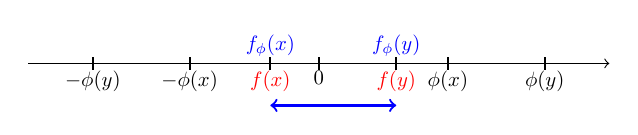
\begin{tikzpicture}[scale=0.82,every node/.style={scale=0.75}]
      \draw[->] (-4.5, 0) -- (4.5, 0);
      \foreach \x in {-3.5,-2,0, -0.75,1.2, 2,3.5} {
        \draw[thick] (\x, -0.1) -- (\x, 0.1);
      }
      \node[below] at (2, 0) {$\phi(x)$};
      \node[below] at (3.5, 0) {$\phi(y)$};
      \node[below] at (-2, 0) {$-\phi(x)$};
      \node[below] at (-3.5, 0) {$-\phi(y)$};
      \node[below] at (0, 0) {$0$};
      \node[below,red] at (-0.75, 0) {$f(x)$};
      \node[above,blue] at (-0.75, 0) {$f_\phi(x)$};
      \node[below,red] at (1.2, 0) {$f(y)$};
      \node[above,blue] at (1.2, 0) {$f_\phi(y)$};
      \draw[<->, thick, blue] (-0.75, -0.65) -- (1.2, -.65);
    \end{tikzpicture}
    \caption{Case 1}
\end{subfigure}
\begin{subfigure}[t]{0.49\textwidth}
    \centering
    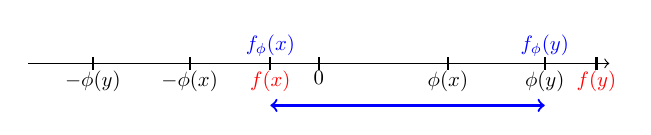
\begin{tikzpicture}[scale=0.82,every node/.style={scale=0.75}]
      \draw[->] (-4.5, 0) -- (4.5, 0);
      \foreach \x in {-3.5,-2,0, -0.75, 2, 4.3,3.5} {
        \draw[thick] (\x, -0.1) -- (\x, 0.1);
      }
      \node[below] at (2, 0) {$\phi(x)$};
      \node[below] at (3.5, 0) {$\phi(y)$};
      \node[below] at (-2, 0) {$-\phi(x)$};
      \node[below] at (-3.5, 0) {$-\phi(y)$};
      \node[below] at (0, 0) {$0$};
      \node[below,red] at (-0.75, 0) {$f(x)$};
      \node[above,blue] at (-0.75, 0) {$f_\phi(x)$};
      \node[below,red] at (4.3, 0) {$f(y)$};
      \node[above,blue] at (3.5, 0) {$f_\phi(y)$};
      \draw[<->, thick, blue] (-0.75, -.65) -- (3.5, -.65);
    \end{tikzpicture}
    \caption{Case 2}
\end{subfigure}

\vspace{1em}

\begin{subfigure}[t]{0.49\textwidth}
    \centering
    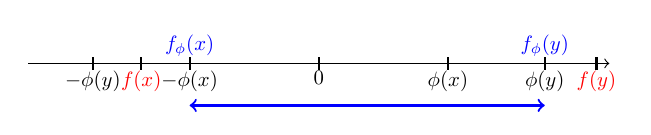
\begin{tikzpicture}[scale=0.82,every node/.style={scale=0.75}]
      \draw[->] (-4.5, 0) -- (4.5, 0);
      \foreach \x in {-3.5,-2,0, -2.75, 2, 4.3,3.5} {
        \draw[thick] (\x, -0.1) -- (\x, 0.1);
      }
      \node[below] at (2, 0) {$\phi(x)$};
      \node[below] at (3.5, 0) {$\phi(y)$};
      \node[below] at (-2, 0) {$-\phi(x)$};
      \node[below] at (-3.5, 0) {$-\phi(y)$};
      \node[below] at (0, 0) {$0$};
      \node[below,red] at (-2.75, 0) {$f(x)$};
      \node[above,blue] at (-2, 0) {$f_\phi(x)$};
      \node[below,red] at (4.3, 0) {$f(y)$};
      \node[above,blue] at (3.5, 0) {$f_\phi(y)$};
      \draw[<->, thick, blue] (-2, -.65) -- (3.5, -.65);
    \end{tikzpicture}
    \caption{Case 3}
\end{subfigure}
\begin{subfigure}[t]{0.49\textwidth}
    \centering
    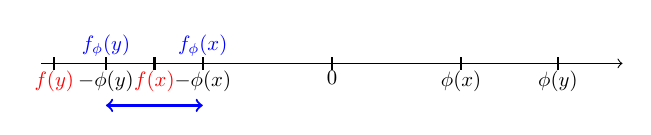
\begin{tikzpicture}[scale=0.82,every node/.style={scale=0.75}]
      \draw[->] (-4.5, 0) -- (4.5, 0);
      \foreach \x in {-3.5,-2,0, -2.75, 2, -4.3,3.5} {
        \draw[thick] (\x, -0.1) -- (\x, 0.1);
      }
      \node[below] at (2, 0) {$\phi(x)$};
      \node[below] at (3.5, 0) {$\phi(y)$};
      \node[below] at (-2, 0) {$-\phi(x)$};
      \node[below] at (-3.5, 0) {$-\phi(y)$};
      \node[below] at (0, 0) {$0$};
      \node[below,red] at (-2.75, 0) {$f(x)$};
      \node[above,blue] at (-2, 0) {$f_\phi(x)$};
      \node[below,red] at (-4.3, 0) {$f(y)$};
      \node[above,blue] at (-3.5, 0) {$f_\phi(y)$};
      \draw[<->, thick, blue] (-2, -.65) -- (-3.5, -.65);
    \end{tikzpicture}
    \caption{Case 4}
\end{subfigure}
\caption{Diagrams showing that $\left|f_\phi(x) - f_\phi(y)\right| \leq \max\left(\left|f(x) - f(y)\right|,\left|\phi(x) - \phi(y)\right| \right)$ .}
\label{fig:comparison-lip-diagram}
\end{figure}
\end{center}
    By construction $|f_\phi| \leq \phi$. This function is also Lipschitz since both $f$ and $\phi$ are Lipschitz, see the diagrams in Figure \ref{fig:comparison-lip-diagram}.
    We get:
    \begin{align*}
        \brac{f,\bar{\mu}^m - \bar{\nu}^m} = \brac{f_\phi,\bar{\mu}^m - \bar{\nu}^m} + \brac{f_\phi-f,\bar{\mu}^m - \bar{\nu}^m}.
    \end{align*}
    
    Notice that for all $x_0 \in \XF$ replacing $f$ by $f - f(x_0)$ does not change the value of $\brac{f,\bar{\mu}^m - \bar{\nu}^m}$ and therefore we can choose an $f$ such that $f(x_0) = 0$. Let $\varepsilon > 0$ and $x_0$ be such that $\phi(x_0) \leq \varepsilon$, take a function $f$ such that $Lip(f) \leq 1$ and $f(x_0) = 0$ then 
    \[
    |f(x)| = |f(x) - f(x_0)| \leq d(x,x_0) \leq \phi(x) + \phi(x_0) \leq \phi(x) + \varepsilon.
    \]
    From this we can deduce:
    \[
    |f_\phi(x) - f(x)| = \max\left(0,|f(x)| - \phi(x) \vphantom{A^2}\right) \leq \phi(x_0) \leq \varepsilon.
    \]
    And finally:
    \begin{align*}
        \brac{f,\bar{\mu}^m - \bar{\nu}^m} &\leq \brac{f_\phi,\bar{\mu}^m - \bar{\nu}^m} + \varepsilon\left(\bar{\mu}^m(\XF) + \bar{\nu}^m(\XF)\right)\\
        &\leq \sup\limits_{\substack{Lip(f) \leq 1,\\ |f| \leq \phi}} \brac{f,\bar{\mu}^m - \bar{\nu}^m} + 2m\varepsilon .
    \end{align*}
    That being true for all $\varepsilon > 0$ we get the equality allowing us to pass to the supremum value on the LHS yields the desired result.

    Step $2$: We start by showing:
    \begin{align*}
        \sup\limits_{\substack{Lip(f) \leq 1,\\ |f| \leq \phi}} \brac{f,\bar{\mu}^m - \bar{\nu}^m} \leq \sup\limits_{\substack{Lip(f) \leq 1,\\ |f| \leq \phi}} \brac{f,\mu - \nu} + \left|\vphantom{A^2}\mu(\XF) - \nu(\XF) \right|
    \end{align*}
    Let us take a Lipschitz function $f$ such that $|f| \leq \phi$:
    \begin{align*}
        \brac{f,\bar{\mu}^m - \bar{\nu}^m} &= \brac{f,\mu - \nu} + f(\partial) \left(\mu(\XF) - \nu(\XF)\vphantom{A^2}\right).
    \end{align*}
    We have that for all $x_0 \in \XF$:
    \[
    |f(\partial)| = \left|\vphantom{A^{\int_0}}f(\partial) - \phi(x_0) + \phi(x_0)\right| \leq 2\phi(x_0) + 1
    \]
    And therefore $|f(\partial)| \leq 1$ since we can take $x_0$ such that $\phi(x_0) \leq \varepsilon$ for all $\varepsilon > 0$ ending step $2$.
    
    Step $3$: We prove the reverse inequality. In the previous step we showed that for all $f$ such that $Lip(f) \leq 1$ and $|f| \leq \phi$ we had that $|f(\partial)| \leq 1$. Therefore:
    \begin{align*}
        \brac{f,\mu - \nu} + f(\partial) \left(\mu(\XF) - \nu(\XF)\vphantom{A^2}\right) \leq \brac{f,\mu - \nu} + \left|\mu(\XF) - \nu(\XF)\vphantom{A^2}\right|.
    \end{align*}
    We can reach part of the optimum by choosing a function $\tilde{f} = f$ on $\XF$ and such that $\tilde{f}(\partial) = sign(\mu(\XF) - \nu(\XF))$. This function is Lipschitz with the right constant, for $x \in \XF$:
    \begin{align*}
        \left|\tilde{f}(x) - \tilde{f}(\partial)\right| \leq  \left|\tilde{f}(x)\right| + \left|\tilde{f}(\partial)\right| \leq \phi(x) + 1.
    \end{align*}
    We have that:
    \begin{align*}
        \brac{f,\mu - \nu} + \left|\vphantom{A^2}\mu(\XF) - \nu(\XF) \right| &= \brac{f,\mu - \nu} + sign(\mu(\XF) - \nu(\XF))\left(\vphantom{A^2}\mu(\XF) - \nu(\XF) \right)\\
        &=  \brac{\tilde{f},\mu - \nu} + \tilde{f}(\partial)\left(\vphantom{A^2}\mu(\XF) - \nu(\XF) \right)\\
        &= \brac{\tilde{f},\bar{\mu}^m - \bar{\mu}^m} \\
        &\leq \sup\limits_{\substack{Lip(f) \leq 1,\\ |f| \leq \phi}} \brac{f,\bar{\mu}^m - \bar{\mu}^m} .
    \end{align*}
    We finish this step and this proof by going to the sup on LHS.
\end{proof}
\begin{remark}
A common approach to generalizing the Wasserstein distance to positive measures of distinct mass is to define:
\begin{align*}
    W_1(\bar{\mu}^m, \bar{\nu}^m) = \sup_{\substack{Lip(f) \leq 1\\ f(x_0) = 0}} \brac{f, \mu - \nu} + \left| \mu(\XF) - \nu(\XF) \right|,
\end{align*}
for some fixed base point $x_0 \in \XF$, without requiring the domination condition involving a function $\phi$ (see \textcolor{red}{REF}). In this setting, if we choose $\phi(x) = d(x, x_0)$, both definitions coincide.

However, our formulation is more flexible. It allows for functions of the form $\phi(x) = \lim_{x_0 \to x_a} d(x, x_0)$, where $x_a$ may lie outside of $\XF$. For example, consider the distance that we are interested in this work \(d_\alpha(x, y) = |x^{-\alpha} - y^{-\alpha}|\) on \(\RRP\), with \(\alpha \geq 0\). Then a natural choice is \(\phi(x) = x^{-\alpha}\), which corresponds to the limit \(x_a = +\infty\), a point not contained in \(\RRP\).
\end{remark}

We emphasize that the distance $W_1(\bar{\mu}^m, \bar{\nu}^m)$ defined in the previous proposition is independent of the choice of $m$, and moreover, it defines a valid distance on the space $\MC^+_{\phi}(\XF)$.

\begin{definition}\label{def:Wasserstein-general}
We define the \emph{$\phi$-Wasserstein distance} on $\MC^+_{\phi}(\XF)$, denoted $W_{\phi}$, as the distance introduced in the previous proposition:
\begin{align*}
    W_{\phi}(\mu, \nu) := \sup_{\substack{Lip(f) \leq 1\\ |f| \leq \phi}} \brac{f, \mu - \nu} + \left| \mu(\XF) - \nu(\XF) \right|.
\end{align*}
\end{definition}
This distance can be generalized to signed measures:
\begin{definition}\label{def:Wasserstein-general-signed}
    We define the \emph{$\phi$-Wasserstein-$1$ distance} on $\MC_{\phi}(\XF)$, denoted $W_{1,\phi}$, as:
\begin{align*}
    W_{\phi}(\mu, \nu) := \sup_{\substack{Lip(f) \leq 1\\ |f| \leq \phi}} \brac{f, \mu - \nu} + \left| \mu(\XF) - \nu(\XF) \right|.
\end{align*}
\end{definition}
It is easy to check the triangular inequality. It stills shares the Wasserstein structure given that for $\mu,\nu \in \MC_{\phi}(\XF)$ let $\mu^+,\mu^-$ and $\nu^+,\nu^-$ respectively the Jordan decomposition of $\mu$ and $\nu$ we have:
\begin{align*}
    W_{\phi}(\mu, \nu) = W_{\phi}(\mu^+ + \nu^-, \nu^+ + \mu^-)\ ,
\end{align*}
and this distance is therefore well-posed. One could also remark that $W_{\phi}(\mu,0)$ defines a norm on $\MC_{\phi}(\XF)$, this is very remniscient of the the flat norm given by Villani in \cite{villani2008optimal}.

\subsubsection{For the distance \(d_\alpha\)}
In this case all distances are equivalent and functions have a limit in $+\infty$ \red{A completer}.

\subsection{Derivatives on spaces of measures}
In this section we define the flat derivative of measures. We define them in the same fashion as in \cite{martiniKolmogorovEquationsSpaces2023} that takes inspiration from its presentation in \cite{cardaliaguet2019master,carmona2018probabilistic}.
\begin{definition}
    Let $E$ be a polish space, $F: \MC(E) \to \RR$ be a continuous function we say that $F$ has a flat derivative if there exists a function $\delta_{\mu}F :\MC(E) \times E\to \RR $ such that for all $\mu,\nu \in \MC(E)$:
    \[ F(\mu) - F(\nu) = \int_0^1 \int_E \delta_\mu F(\theta \mu + (1-\theta)\nu,x)\left(\mu - \nu\right)(\dd x)\dd \theta\]
\end{definition}
We need the same definition but this time for functional from a space of measure to another space of measures.
\begin{definition}
     Let $E$ be a Polish space, $\varphi: \MC(E) \to \MC(E)$ be a continuous function we say that $\varphi$ has a flat derivative if there exists, a continuous function $\delta_{\mu}\varphi :\MC(E) \times E\to \MC(E)$ such that for all $\mu,\nu \in \MC(E)$ and for all $f\in C_b(E)$ \red{Attention, on pourrait demander pour tout $f\in L^1(\mu) \cap L^1(\nu)$ mais il faudrait vérifier que tout fonctionne bien}:
     \begin{itemize}
         \item The function
         \[x\to \sup_{\theta \in [0,1]} |\langle f, \partial_\mu\varphi(\theta \mu + (1-\theta) \nu,x) \rangle| \in L^1(\mu) \cap L^1(\nu).\]
        \item The following equality holds :
            \[ \left\langle f,\varphi(\mu) - \varphi(\nu) \right\rangle= \int_0^1 \int_E \left\langle f,\delta_\mu \varphi(\theta \mu + (1-\theta)\nu,x)\right\rangle\left(\mu - \nu\right)(\dd x)\dd \theta.\]
     \end{itemize}
\end{definition}
We give a formulation of the chain rule.
\begin{proposition}
    Assume that $\delta_\mu F$ is bounded and $\delta_\mu\varphi$ is bounded in total variation. For all \(x\in E\), \(\mu \mapsto \delta_u F(\mu,x)\) and \(\mu \mapsto \delta_u F(\mu,x)\) are continuous. Then \(F\circ \varphi\) has a flat derivative and it is equal to:
    \[
    \delta_\mu F\circ \varphi : \left(\mu,x \right) \mapsto \brac{\delta_\mu  F(\mu,.),\delta_\mu\varphi(\mu,x)}.
    \]
\end{proposition}
\begin{proof}
    Let $\mu,\nu \in \MC(E)$, we define the following function for $\theta \in (0,1)$:
    \[
        g(\theta) =  F\left(\varphi(\theta\mu + (1 - \theta)\nu)\right).
    \]
    We will show that $g$ is differentiable and compute its derivative. One can then conclude by simply noticing that :
    \[ F(\varphi(\mu)) - F(\varphi(\nu)) = \int_0^1 g'(\theta) \dd \theta.\]
    Let $h > 0$, we take advantage of the bracket notation:
    \[ 
    g(\theta + h) - g(\theta) = F\left(\varphi\left([\mu,\nu]^{\theta + h}\right)\right) -F\left(\varphi\left([\mu,\nu]^{\theta}\right)\right)
    \]
    By using the differentiability of $F$ we get:
    \begin{multline*}
    g(\theta + h) - g(\theta) =\\ \int_0^1 \brac{\delta_\mu F\left(\left[\varphi\left([\mu,\nu]^{\theta + h}\right),\varphi\left([\mu,\nu]^{\theta}\right)\right]^{\lambda_1}, . \right),\varphi\left([\mu,\nu]^{\theta + h}\right) - \varphi\left([\mu,\nu]^{\theta}\right)} \dd \lambda_1.
    \end{multline*}
    Now by differentiability of $\varphi$ we get:
    \begin{multline*}
        g(\theta + h) - g(\theta) =\\
        h\int_0^1 \int_0^1\int_E \brac{\delta_\mu F\left(\left[\varphi\left([\mu,\nu]^{\theta + h}\right),\varphi\left([\mu,\nu]^{\theta}\right)\right]^{\lambda_1}, . \right),\delta_\mu \varphi\left(\left[ [\mu,\nu]^{\theta + h}, [\mu,\nu]^{\theta }\right]^{\lambda_2} ,x\right)}
        \\
        (\mu-\nu)(\dd x) \dd \lambda_2 \dd \lambda_1. 
    \end{multline*}
    Notice first that \(\left[\varphi\left([\mu,\nu]^{\theta}\right),\varphi\left([\mu,\nu]^{\theta}\right)\right]^{\lambda_1} = \varphi\left([\mu,\nu]^{\theta}\right)\).
    \red{A terminer}
\end{proof}

\section{The Smoluchovski coagulation equation and its derivative}\label{section:well-posedness-SCE}
% Recall the Smolochowski coagulation equation of kernel $K_\alpha$ \eqref{eq:SCE} for all $f \in C_b(\RRP)$:
% \begin{equation*}
%    \brac{f,\mu_t}  = \brac{f,\mu} +  \dfrac12\int_0^t \brac{K_\alpha f,\mu_s^{\otimes 2}} \dd s.
% \end{equation*}
The goal of this section is to prove that the Smoluchovski coagulation equation is well-posed as stated in Lemma~\ref{lem:well_posedness_smol_eq}. And that the existence of a flat derivaitve and well-posedness of its equation as in Lemma~\ref{lem:derivative-existence-and-eq}.



% that it is well-posed in the sense that for $\mu \in \MC^+_{\psi_2}(\RRP)$ it has a unique solution in:
% \[
% C\left([0,T]: \MC^+_{\psi_2}(\RRP)\right).
% \]
% Let us denote by $\Proc{\varphi_t(\mu)}$ said solution. If $\mu \in \MC^+_{\psi_3}(\RRP)$ we show that for all $t \geq 0,\ \mu \mapsto \varphi_t(\mu)$ has a flat derivaitve and it is the unique solution of equation for all $z \in \RRP,\  f \in C_b(\RRP)$:
% \begin{equation*}
%     \brac{f,\delta_\mu \varphi_t(\mu;z)} = f(z) + \int_0^t \brac{K_\alpha f, \varphi_s(\mu)\otimes \delta_\mu \varphi_s(\mu;z) } \dd s
% \end{equation*}
% in
% \[
% C\left([0,T]: \MC^+_{\psi_3}(\RRP)\right).
% \]
\subsection{Smoluchovski}
Expliquer ce que l(on) fait dans cette section.

\subsubsection{Some bounds}
In this section we assume the well-posedness of both the Smoluchovski coagulation equation in $C([0,T]: \MC_{\psi_2}(\RRP))$. We recall that the solution of the \(\SCE\) is a positive measure. The first lemma give a result of stability of solutions of the \(\SCE\) and hold for all kernels.
\begin{lemma}\label{lem:sub-add-bounf-smol}
    Let $\phi$ be a sub-multiplicative function meaning that for all $\lambda \geq 1$, $\phi(\lambda x) \leq \lambda \phi(x)$; If $\mu_0 \in \MC^+_{\phi}(\RRP)$ and for all $t\in[0,T]$, $\mu_t \in \MC^+_{\phi}(\RRP)$, then for all $t\geq 0$.
\end{lemma}
\begin{proof}
    The proof is straight-forward, since $\mu_t$ is non-negative for all $t\geq 0$:
    \begin{align*}
        \|\mu_t\|_{\phi} = \brac{\phi,\mu_t} = \brac{\phi,\mu_0} + \int_0^t \brac{K\phi,\mu_s^{\otimes 2}}\dd s.
    \end{align*}
    All sub-multiplicative function are also sub additive meaning for all $x,y \in \RRP$ \(\phi(x+y) \leq \phi(x) + \phi(y)\) indeed
    \begin{multline*}
        \phi(x+y) = \phi\left(x\vee y \times \dfrac{x+y}{x\vee y} \right) \leq \dfrac{x+y}{x\vee y}\phi\left(x\vee y \right) = \dfrac{x\vee y +x\wedge y}{x\vee y}\phi\left(x\vee y \right) \\
         = \phi\left(x\vee y \right) + \dfrac{x\wedge y}{x\vee y} \phi\left(x\wedge  y \times \dfrac{x\vee  y}{x\wedge  y} \right) \leq \phi\left(x\vee y \right) +  \phi\left(x\wedge  y \right) = \phi\left(x \right) +  \phi\left(y \right).
    \end{multline*}
    Therefore
    \begin{align*}
        \brac{K\phi,\mu_s^{\otimes 2}} = \int_{\RRP\times \RRP} K(x,y) \left(\phi(x+y) - \phi(x) - \phi(y)\right) \mu_s(\dd x) \mu_s (\dd y) \leq 0.
    \end{align*}
    So $ \|\mu_t\|_{\phi} \leq  \|\mu_0\|_{\phi}$ ending the proof.
\end{proof}
Now we know that spaces of measures defined by a finite measure of the function $\phi$ are a good setting. Note that the following functions are sub multiplicative:
\begin{align*}
    x \mapsto x^\gamma,\quad,x \mapsto e^{cx^\gamma},\quad  \gamma\in(-\infty,0], \quad c \geq 0. 
\end{align*}
Note also that any positive linear combination of sub-multiplicative function is also sub multiplicative. Therefore all the measure spaces we defined in our introduction are stable for the $\SCE$. The previous result told us that $t \mapsto \|\mu_t\|_{\phi}$ is non-increasing, the next proposition gives a more precise estimation of this damping for some particular $\phi$'s. 
\begin{lemma}\label{lem:bound_smol_1}
    Let $\mu_t$ be the solution of the Smoluchovski coagulation equation for the kernel $K_\alpha$ started from measure $\mu$. For all $t\geq 0$ we have:
    \begin{enumerate}[label=(\roman*)]
        \item \( \left\langle 1, \mu_t \right\rangle \leq \frac{\left\langle 1, \mu \right\rangle}{\left(1 + (1 + \alpha)\left\langle x, \mu \right\rangle^{-\alpha} \left\langle 1, \mu \right\rangle^{1 + \alpha} t \right)^{\frac{1}{1 + \alpha}}}.\)
        \item \(\left\langle x^{-\alpha}, \mu_t \right\rangle \leq \frac{\left\langle x^{-\alpha}, \mu \right\rangle}{1 + C_\alpha\left\langle x^{-\alpha}, \mu \right\rangle t }\), where $C_\alpha = 2 - 2^{-\alpha}$
    \end{enumerate}
    % \begin{align*}
    %     \left\langle 1, \mu_t \right\rangle &\leq \dfrac{\left\langle 1, \mu \right\rangle}{\left(1 + (1 + \alpha)\left\langle x, \mu \right\rangle^{-\alpha} \left\langle 1, \mu \right\rangle^{1 + \alpha} t \right)^{\frac{1}{1 + \alpha}}}.
    % \end{align*}
\end{lemma}
\begin{proof}
    $(i)$ Let us write the $ODE$ verified by our quantity of interest:
    \begin{align}
        \dfrac{\dd}{\dd t} \left\langle 1, \mu_t \right\rangle
        &= -\dfrac12\int_{\RR^{+,*} \times \RR^{+,*} } K_\alpha(x,y) \mu_t^{\otimes 2} (\dd x, \dd y) \nonumber\\
        &= -\left\langle 1, \mu_t \right\rangle \left\langle x^{-\alpha}, \mu_t \right\rangle. \label{eq:proof:bound_1_smol}
    \end{align}
    To continue we bound below $\left\langle x^{-\alpha}, \mu_t \right\rangle$. By positivity of $\varphi$, $\frac{\mu_t}{\left\langle 1, \mu_t\right\rangle}$ is a probability measure on $\RR^{+,*}$ and the function $x\mapsto x^{-\alpha}$ is convex on $\RR^{+,*}$ therefore by Jensen's inequality we have:
    \begin{align*}
        \dfrac{\left\langle x^{-\alpha},\mu_t \right\rangle}{\left\langle 1, \mu_t\right\rangle} \geq  \left(\dfrac{\left\langle x,\mu_t \right\rangle}{\left\langle 1, \mu_t\right\rangle}\right)^{-\alpha} \implies
        \left\langle x^{-\alpha},\mu_t \right\rangle \geq \left\langle x,\mu_t \right\rangle^{-\alpha} \left\langle 1, \mu_t\right\rangle^{1 + \alpha}.
    \end{align*}
    Now recall that for all $t \geq 0$ the total mass remains constant meaning that $\left\langle x,\mu_t\right\rangle = \left\langle x,\mu\right\rangle$, giving us:
    \begin{align*}
        \left\langle x^{-\alpha},\mu_t \right\rangle \geq \left\langle x,\mu \right\rangle^{-\alpha} \left\langle 1, \mu_t\right\rangle^{1 + \alpha}.
    \end{align*}
    Replacing it in \eqref{eq:proof:bound_1_smol} gets us :
    \begin{align*}
        \dfrac{\dd}{\dd t} \left\langle 1, \mu_t \right\rangle
        \leq -\left\langle x,\mu \right\rangle^{-\alpha}\left\langle 1, \mu_t \right\rangle^{2 + \alpha}.
    \end{align*}
    We conclude by using lemma \red{ajouter le lemme pour $u' \leq -a u^\gamma$, $\gamma \geq 1$}.

    $(ii)$ The function $x \mapsto x^{-\alpha}$ is convex on $\RR^{+,*}$, so:
    \begin{align*}
        \left(\dfrac{x + y}{2}\right)^{-\alpha} \leq \dfrac{1}{2}  \left(x^{-\alpha} + y^{-\alpha}\right) \implies 
        \left(x + y\right)^{-\alpha} - x^{-\alpha} - y^{-\alpha} \leq \dfrac{C_\alpha}{2} \left( x^{-\alpha} + y^{-\alpha}\right).
    \end{align*}
    Now from the Smoluchovski coagulation equation we have:
    \begin{align*}
        \dfrac{\dd}{\dd t} \left\langle x^{-\alpha},\mu_t\right\rangle &= \dfrac12\int_{\RR^{+,*}\times \RR^{+,*}} K_\alpha(x,y) \left((x + y)^{-\alpha}- x^{-\alpha} - y^{-\alpha} \right) \mu_t^{\otimes 2}(\dd x, \dd y).
    \end{align*}
    Now by positivity of $\Proc{\mu_t}$ we have:
    \begin{align*}
        \dfrac{\dd}{\dd t} \left\langle x^{-\alpha},\mu_t\right\rangle &\leq -\dfrac{C_\alpha}{2}\int_{\RR^{+,*}\times \RR^{+,*}} \left(x^{-\alpha} + y^{-\alpha} \right)^2 \mu_t^{\otimes 2}(\dd x, \dd y)
        \\
        &= -\dfrac{C_\alpha}{2} \left\langle x^{-\alpha}, \mu_t\right\rangle^2 - \dfrac{C_\alpha}{2}\left\langle x^{-2\alpha}, \mu_t\right\rangle \left\langle 1, \mu_t\right\rangle.
    \end{align*}
   The measure $\frac{\mu_t}{\left\langle 1, \mu_t\right\rangle}$ is a probability measure. By convexity of the square function and Jensen's inequality:
   \begin{align*}
       \left\langle 1, \mu_t\right\rangle\left\langle x^{-2\alpha}, \mu_t\right\rangle \geq \left\langle x^{-\alpha}, \mu_t\right\rangle^2.
   \end{align*}
   Therefore:
    \begin{align*}
        \dfrac{\dd}{\dd t} \left\langle x^{-\alpha},\mu_t\right\rangle &\leq -C_\alpha \left\langle x^{-\alpha}, \mu_t\right\rangle^2.
    \end{align*}
    Finally we conclude with lemma \ref{lem:inequality_ODE_square}:
    \begin{align*}
        \left\langle x^{-\alpha},\mu_t\right\rangle \leq \dfrac{\left\langle x^{-\alpha}, \mu \right\rangle}{1 + C_\alpha\left\langle x^{-\alpha}, \mu \right\rangle t },
    \end{align*}
    giving us the desired result.
\end{proof}
% \begin{proposition}
%     Let $\phi_{e}^c(x) = e^{cx^{-\alpha}}$.
% \end{proposition}
% \begin{proof}
%     We compute:
%     \begin{align*}
%         \dfrac{\dd}{\dd t}\brac{\phi^c,\mu_t} &= \dfrac{1}{2}\int_{\RRP \times \RRP} K_\alpha(x,y)  \left[e^{c(x+y)^{-\alpha}} - e^{cx^{-\alpha}} - e^{cy^{-\alpha}} \right]\mu_t(\dd x) \mu_t( \dd y) \\
%         &\leq -\dfrac{1}{2}\int_{\RRP \times \RRP} K_\alpha(x,y)  e^{cx^{-\alpha}}\mu_t(\dd x) \mu_t( \dd y) \\
%         &= -\dfrac12\brac{1,\mu_t}\int_{\RRP} x^{-\alpha} e^{cx^{-\alpha}}\mu_t(\dd x) - \dfrac12\brac{x^{-\alpha},\mu_t}\brac{\phi^c,\mu_t}.
%     \end{align*}
%     Let us denote $u(c,t) := \brac{\phi^c,\mu_t}$ the previous can be seen as the following inequality:
%     \begin{align*}
%         \partial_t u \leq -\brac{1,\mu_t}\partial_c u - \brac{x^{-\alpha},\mu_t} u.
%     \end{align*}
% \end{proof}
The next lemma gives shows that the solution of the $\SCE$ is Lipschitz with respect to its initial value in a specific weighted norm total variation norm.
\begin{lemma}\label{lem:Lip-smol-TV}
    Let $\mu,\nu \in \MC^+_{\phi_p}(\RRP)$ and denote $\mu_t,\nu_t$ the respective solutions of the $\SCE$ started from $\mu,\nu$ we have:
    \begin{align*}
        \sup\limits_{t \in [0,T]}\| \mu_t - \nu_t\|_{\phi_p} \leq e^{CT\left(\|\mu\|_{\phi_{p+1}} + \|\nu\|_{\phi_{p+1}}\right)}\|\mu- \nu\|_{\phi_p}.
    \end{align*}
\end{lemma}
\begin{proof}
    From lemma \ref{lem:ODE_total_variation_kolo}:
    \begin{multline*}
        \| \mu_t - \nu_t\|_{\phi_p} = \|\mu- \nu\|_{\phi_p} \\
        + \dfrac12\int_0^t \int_{\RRP}\int_{\RRP} K_\alpha(x,y) \left[\phi_p\sigma_s(x+y) - \phi_p\sigma_s(x) - \phi_p\sigma_s(y) \right]\left(\mu_t + \nu_t\right)(\dd x) \left(\mu_t - \nu_t\right)(\dd y).
    \end{multline*}
    where $\sigma_s$ is a density of $\mu_s - \nu_s$ with respect to to $|\mu_s - \nu_s|$. We use the positivity of $\mu_t$ and $\nu_t$: 
    \begin{multline*}
        \| \mu_t - \nu_t\|_{\phi_p} \leq \|\mu- \nu\|_{\phi_p} \\
        + \dfrac12\int_0^t \int_{\RRP}\int_{\RRP} K_\alpha(x,y) \left[\phi_p(x+y) - \phi_p(y) \right]\left(\mu_t + \nu_t\right)(\dd x) \left|\mu_t - \nu_t\right|(\dd y) \\
        + \dfrac12\int_0^t \int_{\RRP}\int_{\RRP} K_\alpha(x,y)\phi_p(x)\left(\mu_t + \nu_t\right)(\dd x) \left|\mu_t - \nu_t\right|(\dd y).
    \end{multline*}
    Finally since $\phi_p(x+y) - \phi(y) \leq \phi_p(x)$ we have:
    \begin{align*}
        \| \mu_t - \nu_t\|_{\phi_p} &\leq \|\mu- \nu\|_{\phi_p} + \int_0^t \int_{\RRP}\int_{\RRP} K_\alpha(x,y)\phi_p(x)\left(\mu_s + \nu_s\right)(\dd x) \left|\mu_s - \nu_s\right|(\dd y)\\
        &\leq \|\mu- \nu\|_{\phi_p} + C\left(\|\mu\|_{\phi_{p+1}} + \|\nu\|_{\phi_{p+1}}\right) \int_0^t \|\mu_s - \nu_s \|_{\phi_p}\dd s.
    \end{align*}
    We use a Gronwall's lemma ending the proof.
\end{proof}
% \begin{proof}
%     We denote $\|\cdot\|_{\psi_1}$ by  $\|\cdot\|$ for convenience. From lemma \ref{lem:ODE_total_variation_kolo}:
%     \begin{multline*}
%         \| \mu_t - \nu_t\| = \|\mu- \nu\| \\
%         + \dfrac12\int_0^t \int_{\RRP}\int_{\RRP} K_\alpha(x,y) \left[\psi_1\sigma_s(x+y) - \psi_1\sigma_s(x) - \psi_1\sigma_s(y) \right]\left(\mu_s + \nu_s\right)(\dd x) \left(\mu_s - \nu_s\right)(\dd y) \dd s.
%     \end{multline*}
%     where $\sigma_s$ is a density of $\mu_s - \nu_s$ with respect to to $|\mu_s - \nu_s|$ so that $\sigma_s(\mu_s - \nu_s) = |\mu_s - \nu_s|$. We use the positivity of $\mu_t ,\nu_t$ and the definition of $\sigma_t$: 
%     \begin{align*}
%         \| \mu_t - \nu_t\| 
%         &\leq \|\mu- \nu\| + \dfrac12\int_0^t \int_{\RRP}\int_{\RRP} K_\alpha(x,y)\psi_1(x)\left(\mu_s + \nu_s\right)(\dd x) \left|\mu_s - \nu_s\right|(\dd y) \dd s.
%     \end{align*}
%     where we used that $\psi_1(x + y) \leq \psi_1(y)$ for all $x,y \geq 0$. Finally we have:
%     \begin{align*}
%         \dfrac{\dd}{\dd t}\| \mu_t - \nu_t\| \leq   C\brac{\psi_2,\mu_t + \nu_t}\|\mu_t - \nu_t\| \leq C\left(\|\mu\|_{\psi_2} + \|\mu\|_{\psi_2}\right)\|\mu_t - \nu_t\|.
%     \end{align*}
%     We conclude with a Gronwall's lemma.
% \end{proof}
% \begin{corollary}\label{cor:Lip-smol-TV}
%     Let $\psi_n : x\mapsto 1 + x^{-n\alpha}$. Let $p \geq 2$ and $\mu,\nu \in \MC^+_{\phi_{p+1}}(\RRP)$ and denote $\mu_t,\nu_t$ the respective solutions of the $\SCE$ started from $\mu,\nu$ we have:
%     \begin{align*}
%         \sup\limits_{t \in [0,T]}\| \mu_t - \nu_t\|_{\phi_p} \leq \left(1 + T e^{C\left(\|\mu\|_{\phi_{p + 1}} + \|\nu\|_{\phi_{p+1}}\right)T}\right)\|\mu- \nu\|_{\psi_1}.
%     \end{align*}
%     The functions $\phi_p$ could be replaced by $\psi_p$.
% \end{corollary}

\subsubsection{Well-posedness of the Smoluchovski coagulation equation}
In this section we show that the $\SCE$ is well posed and give some useful bounds on it. Because of the singularity of our kernel we start by considering a cut-off equation where we sever the initial value away from $0$, we take $\mu^\varepsilon = \mu\mathds{1}_{[\varepsilon,\infty)}$. And call $\mu^\varepsilon_t$ the solution to the corresponding equation:
\begin{equation}\label{eq:cutoff_SCE}
    \brac{f, \mu^\varepsilon_t} = \brac{f,\mu^\varepsilon} + \dfrac12\int_0^t \brac{K_\alpha f,\left(\mu^\varepsilon_s\right)^{\otimes 2}} \dd s.
\end{equation}
The mass of newly formed particles can only be greater than the smallest initial available mass because this equation describes pure coagulation, as such the support of $\mu^\varepsilon$ is included in $[\varepsilon,\infty)$. We will later make $\varepsilon$ tend to zero in order to build a solution to the $\SCE$.

We will start by showing that \eqref{eq:cutoff_SCE} has a unique solution on a small interval of time. Then we will extend the temporal domain using some  bounds proved before.
\begin{proposition}\label{prop:well-posedness-cutoff-smol}
    Let $\mu \in \MC^+_{\phi_p}(\RRP)$, for all $T > 0$ equation \eqref{eq:cutoff_SCE} has a unique solution in $C\left([0,T]:\MC^+_{\phi_p}(\RRP)\right)$. Furthermore the support of aforesaid solution is included in $[\varepsilon,\infty)$ for all $t \in [0,T]$.
\end{proposition}

This proof is based on a classical fixed point theorem in a complete space. We will first show that the solution exists on a small time interval using a fixed point method in the following space of signed measures:
    \[ \MC^{\varepsilon,M}_{\phi_p}(\RRP) = \left\lbrace \mu \in \MC_{\phi_p}(\RRP) ,\quad \|\mu \|_{\phi_p}\leq M,\quad supp(\mu) \subset [\varepsilon,\infty)\right\rbrace. \]
It is a closed subspace of $\MC_{\phi_p}(\RRP)$ and therefore is complete for the associated weighted norm. Then we preform a second fixed point to show that if the initial measure is positive then the solution stays positive for all time. Both intermediate results are given in the lemma below. 
\begin{lemma}
    Assume that the initial measure $\mu$ is such that, $\| \mu\|_{\phi_p} \leq \frac{M}{2}$, there exists a time $T^{\varepsilon,M} > 0$ such that equation \eqref{eq:cutoff_SCE} has a unique solution in $C\left([0,T^{\varepsilon,M}]:\MC^{+,\varepsilon,M}_{\phi_p}(\RRP)\right)$. 
\end{lemma}
\begin{proof}
    We introduce the functional:
    \begin{align*}
    \Gamma^\varepsilon : 
    \left\lbrace 
    \begin{aligned}
        C\left([0,T]:\MC^{\varepsilon,M}_{\phi_p}(\RRP) \right) &\to C\left([0,T]:\MC^{\varepsilon,M}_{\phi_p}(\RRP) \right)\\
         m & \mapsto \Gamma^\varepsilon(m)
    \end{aligned}
    \right.,
    \end{align*}
    defined for all $f \in C_b(\RRP)$, for all $t \geq 0$ by:
    \begin{align*}
        \brac{f,\Gamma^\varepsilon(m)_t}= \brac{f,\mu^\varepsilon} + \dfrac12\int_0^t \brac{K_\alpha f,\left(m_s\right)^{\otimes 2}} \dd s.
    \end{align*}
    Claim $1$: For $T$ small enough the functional $\Gamma^\varepsilon$ is well defined. First of all it is quite clear that if $m \in C\left([0,T]:\MC^{\varepsilon,M}_{\phi_p}(\RRP) \right)$ the support of $\Gamma^\varepsilon(m)_t$ is included $[\varepsilon,\infty)$ for all $t$. Let $|f| \leq \phi_p$ we have:
    \begin{align*}
        \brac{f,\Gamma^\varepsilon(m)_t} &\leq \|\mu^\varepsilon\|_{\phi_p} + C\varepsilon^{-\alpha}\int_0^t \brac{\phi_p,|m_s|}^2 \dd s 
    \end{align*}
    where $C$ is a constant. And therefore:
    \begin{align*}
        \sup\limits_{t\in [0,T]} \| \Gamma^\varepsilon(m)_t\|_{\phi_p} 
        &\leq \|\mu\|_{\phi_p} + C\varepsilon^{-\alpha} T M^2.
    \end{align*}
    Since we assumed that $\|\mu\|_{\phi_p} \leq \frac{M}{2}$ it suffices to choose $T = \dfrac{1}{2\varepsilon^{-\alpha}MC}$. Finally by boundedness of the integrand in time it follows that $t \mapsto \Gamma^\varepsilon(m)_t$ is continuous thus showing the claim.

    Claim 2 : For $T$ small enough the operator $\Gamma^\varepsilon$ is a contraction. Let $m^1$ and $m^2$ be in $\MC^{\varepsilon,M}_{\phi_p}\left(\RRP\right)$. Let $|f| \leq \phi$, we have:
    \begin{align*}
        \brac{f,\Gamma^\varepsilon(m^1)_t - \Gamma^\varepsilon(m^2)_t}
        &= \dfrac{1}{2}\int_0^t \brac{Kf,\left(m^1_s + m^2_s\right)\otimes\left( m^1_s - m^2_s\right)} \dd s \\
        &\leq C\varepsilon^{-\alpha}\int_0^t \|m^1_s + m^2_s\|_{\phi_p} \|m^1_s - m^2_s\|_{\phi_p}\dd s .
    \end{align*}
    Therefore we have:
    \begin{align*}
        \sup\limits_{t \in [0,T]} \|\Gamma^\varepsilon(m^1)_t - \Gamma^\varepsilon(m^2)_t\|_{\phi_p} \leq 2\varepsilon^{-\alpha} CMT\sup\limits_{t \in [0,T]} \|m^1_t - m^2_t\|_{\phi_p} .
    \end{align*}
    Taking $T = \frac{1}{4\varepsilon^{-\alpha}CM}$ proves the claim. Now let $T^{\varepsilon,M} = \frac{1}{4\varepsilon^{-\alpha}CM}$, the Banach contraction theorem give us existence and uniqueness of a solution to equation \eqref{eq:cutoff_SCE} defined on the time interval $[0,T^{\varepsilon,M}]$ with values in $\MC^{\varepsilon,M}_{\phi_p}\left(\RRP\right)$. It remains to show that this solution is positive, let us call it $\mu_t^\varepsilon$. Consider the function:
    \[
    h^\varepsilon_t(x) = \exp\left(\int_0^t\int_{\RRP}K_\alpha (x,y) \mu^\varepsilon_s(\dd y) \dd s\right).
    \]
    We have the following relation \red{Ajouter petite proposition pour justifier la dérivation.}:
    \begin{align*}
        \dfrac{\dd}{\dd t}\brac{fh^\varepsilon_t,\mu^\varepsilon_t} &= \brac{fh'^{\varepsilon}_t,\mu^\varepsilon_t} + \dfrac{1}{2}\brac{K_\alpha f,\left(\mu^\varepsilon_t\right)^{\otimes 2}}\\
        &= \dfrac{1}{2}\int_{\RRP\times\RRP} K_\alpha(x,y) f(x+y)h^\varepsilon_t(x+y)\mu^\varepsilon_t(\dd x)\mu^\varepsilon_t(\dd y) \\
        &= \brac{f,G_t(h^\varepsilon_t\mu^\varepsilon_t)},
    \end{align*}
    where $G : \MC^{+,\varepsilon,M}_{\phi_p}(\RRP) \to \MC^{+,\varepsilon,M}_{\phi_p}(\RRP)$ is defined by:
    \begin{align*}
        \brac{f,G_t(m)} =  \dfrac{1}{2}\int_{\RRP\times\RRP} K_\alpha(x,y) f(x+y)h^\varepsilon_t(x+y) h^\varepsilon_t(x)^{-1} h^\varepsilon_t(y)^{-1}m(\dd x)m(\dd y).
    \end{align*}
    We want to show that that measure $h^\varepsilon_t\mu^\varepsilon_t$ is positive implying that $\mu^\varepsilon_t$ is positive by construction of $h^\varepsilon_t$. To do so we do a second fixed point. We build a new operator for our second fixed point: 
    \[ \Gamma^{+,\varepsilon} : 
    \left\lbrace 
    \begin{aligned}
        C\left([0,T]:\MC^{+,\varepsilon,M}_{\phi_p}(\RRP) \right) &\to C\left([0,T]:\MC^{+,\varepsilon,M}_{\phi_p}(\RRP) \right)\\
         m & \mapsto \Gamma^{+,\varepsilon}(m)
    \end{aligned}
    \right.,
    \]
    defined for all $f \in C_b(\RRP)$, for all $t \geq 0$ by:
    \begin{align*}
        \brac{f,\Gamma^{+,\varepsilon}(m)_t}= \brac{f,\mu^\varepsilon} + \int_0^t \frac{f,G_s(m_s)}  \dd s.
    \end{align*}
    Claim $3$: For $T$ small enough $\Gamma^{+,\varepsilon}(m)$ is well defined. If $m$ is a map from $[0,T]$ to positive measures it is clear that $\Gamma^{+,\varepsilon}(m)_t$ is positive for all $t\geq 0$. We have that:
    \begin{align*}
        G_s(m_s) \leq C \varepsilon^{-\alpha}\|m_s\|_{\phi_p}^2.
    \end{align*}
    with a reasoning that follows the first fixed point we can show that for $T$ small enough (possibly smaller than previously) the operator $\Gamma^{+,\varepsilon}$ is well defined. 
    Claim $4$: For $T$ small enough $\Gamma^{+,\varepsilon}(m)$ is a contraction. We have:
    \begin{align*}
        \brac{f, \Gamma^{+,\varepsilon}(m^1)_t - \Gamma^{+,\varepsilon}(m^2)_t} \leq C \varepsilon^{-\alpha}\int_0^t \|m^1_s - m^2_s\|_{\phi_p}\|m^1_s + m^2_s\|_{\phi_p} \dd s.
    \end{align*}
    It follows again that for $T$ sufficiently small the operator is a contraction. We now denote $\tilde{T}^{\varepsilon,M}$ the minima of all $4$ times found previously. We use again the Banach contraction theorem with initial measure $\mu$, the obtained fixed point is a positive measure on  $[0,\tilde{T}^{\varepsilon,M}]$. We previously found a unique solution to \eqref{eq:cutoff_SCE} therefore the aforementioned fixed point is $h^\varepsilon_t\mu^\varepsilon_t$, finally implying that $\mu^\varepsilon_t$ is positive on the found time interval.
\end{proof}
\begin{remark}
    Extending the temporal domain of the solution is not straight-forward. The classical technique is to start the equation with initial value the solution taken at time $T^{\varepsilon,M}$. The issue is that this measure belongs to $\MC^{M}_p\left( \RRP\right)$ contrary to the initial value $\mu$ that is in $\MC^{M/2}_p\left( \RRP\right)$. Therefore each time increments will double the bound. This coupled with the dependence of $T^\varepsilon$ with respect to $M$ makes that the maximal time horizon is function of $M$. We need to control the increase in this bound if want to extend the temporal domain of our solution.
\end{remark}
We can easily extend the definition domain because we have uniform bounds on the solution thanks to lemma \ref{lem:sub-add-bounf-smol}.
\begin{proof}[Proof of Proposition \ref{prop:well-posedness-cutoff-smol}]
    Let us denote $M:= \|\mu\|_{\phi_p}$, from the previous lemma we know that we can build a solution to \eqref{eq:cutoff_SCE} on an interval $\left[0,T^{\varepsilon,M}\right]$. By lemma \ref{lem:sub-add-bounf-smol} we have:
    \begin{align*}
        \sup\limits_{t \in \left[0,T^{\varepsilon,M}\right]} \|\mu_t\|_{\phi_p} \leq \|\mu\| = M.
    \end{align*}
    Therefore we can build another solution on interval $\left[T^{\varepsilon,M}, 2T^{\varepsilon,M}\right]$ using the previous lemma. By induction we can build a solution from $[0,T]$ to $\MC^{+,\varepsilon,M}\left(\RRP\right)$ for all $T$ and thanks to the uniformity of the bound we can build it on $\RR^{+}$ by letting $T \to \infty$ ending the proof.
\end{proof}
Now it remains to let $\varepsilon$ go to zero to build a a solution to the $\SCE$ \eqref{eq:SCE}. 
\begin{lemma}[Restated Lemma~\ref{lem:well_posedness_smol_eq}]
    Let $p \geq 2$, and $\mu \in \MC_{\phi_p}^+ (\RRP)$ for all $T \geq 0$ there exists a unique solution to the Smoluchovski equation of kernel $K_\alpha$, said solution is a continuous map from $[0,T]$ to $\mu \in \MC_{\phi_p}^+ (\RRP)$.
\end{lemma}
Our strategy is to show that we can extract from the family of solutions $\left(\Proc{\mu^\varepsilon}\right)_{\varepsilon > 0}$ a Cauchy sequence. Then we will show that this limit is a solution to the Smoluchowski coagulation equation and finally use a Gronwall's lemma to show uniqueness. 
\begin{proof}
    Let $T > 0$ and for all $n\in \NN$, $\varepsilon_n = \frac1n$. By proposition \ref{prop:well-posedness-cutoff-smol} we know that for all $n \in \NN$ the cut-off equation \eqref{eq:cutoff_SCE} has a unique solution in $C\left([0,T]: \MC_{\phi_{p}}^+ (\RRP)\right)$ that we denote by $\Proc{\mu^{\varepsilon_n}}$. We start to show that the aforementioned sequence is Cauchy in the space of continuous maps from $[0,T]$ to $\MC_{\phi_{p-1}}^+ (\RRP)$ with its associated norm. Then we will show that the limit has a moment of order $p$, that it is a solution to the $\SCE$ and the unique one for that matter.
    
    For $\varepsilon_1 < \varepsilon_2$ we have from lemma \ref{lem:Lip-smol-TV} 
    \begin{align*}
        \| \mu_t^{\varepsilon_1}- \mu_t^{\varepsilon_2}\|_{\phi_{p-1}} \leq C(T,\|\mu\|_{\phi_{p}}) \| \mu^{\varepsilon_1}- \mu^{\varepsilon_2}\|_{\phi_{p-1}}.
    \end{align*}
    We exhibit the epsilons like so:
    \begin{align*}
        \| \mu^{\varepsilon_1}- \mu^{\varepsilon_2}\|_{\phi_{p-1}} &= \int\indic{\varepsilon_1 \leq x < \varepsilon_2} \phi_{p-1}(x)\mu(\dd x)\\
        &= \int x^{\alpha} \indic{\varepsilon_1 \leq x < \varepsilon_2} x^{-\alpha}\phi_{p-1}(x)\mu(\dd x)\\
        &\leq C(\varepsilon_2)^\alpha \|\mu\|_{\phi_{p}}.
    \end{align*}
    So for all $p,q \geq N$ we have:
    \begin{align*}
        \sup\limits_{t \in [0,T]} \| \mu_t^{\varepsilon_p}- \mu_t^{\varepsilon_q}\|_{\phi_{p-1}} \leq \dfrac{1}{N^\alpha} C(T,\|\mu\|_{\phi_{p}}) \| \mu\|_{\phi_p},
    \end{align*}
    therefore the sequence is Cauchy, let us denote $\Proc{\mu_t}$ its limit. We show that it is the only solution to the $\SCE$: let $f \in C_b(\RRP)$, for all $\varepsilon > 0$
    \begin{multline*}
        \brac{f,\mu_t} - \brac{f,\mu} - \int_0^t\brac{Kf,\mu_s^{\otimes 2}}\dd s \\
        = \brac{f,\mu_t-\mu_t^\varepsilon} - \brac{f,\mu-\mu^\varepsilon} - \int_0^t\brac{Kf,(\mu_s+ \mu^\varepsilon_s)\otimes (\mu_s - \mu^\varepsilon_s)}\dd s
    \end{multline*}
    therefore
    \begin{multline*}
        \left|\brac{f,\mu_t} - \brac{f,\mu} - \int_0^t\brac{Kf,\mu_s^{\otimes 2}}\dd s\right|\\
        \leq \|\mu_t - \mu_t^\varepsilon\|_{\phi_0} + \|\mu - \mu^\varepsilon\|_{\phi_0} + C\|\mu\|_{\phi_1}\int_0^t \| \mu_s - \mu^\varepsilon_s \|_{\phi_1} \dd s
    \end{multline*}
    and using lemma \ref{lem:Lip-smol-TV}:
    \begin{align*}
        \left|\brac{f,\mu_t} - \brac{f,\mu} - \int_0^t\brac{Kf,\mu_s^{\otimes 2}}\dd s\right| &\leq C(t,\|\mu\|_{\phi_1},\|\mu\|_{\phi_2})\|\mu - \mu^\varepsilon\|_{\phi_1} \\
        &\leq \varepsilon^{\alpha} C(t,\|\mu\|_{\phi_1},\|\mu\|_{\phi_2})\|\mu\|_{\phi_2}.
    \end{align*}
    That being true for all $\varepsilon$ we have that, $\Proc{\mu_t}$ is a solution to the $\SCE$. Uniqueness comes from the lipschitz character of the solution given in lemma \ref{lem:Lip-smol-TV}. Finally we show that it has a moment of order $p$. By lemma \ref{lem:bound_smol_1} we have:
    \begin{align*}
        \sup\limits_{t \in [0,T]} \| \mu_t\|_{\phi_{p}} \leq  \| \mu\|_{\phi_{p}},
    \end{align*}
    concluding this proof.
\end{proof}

\subsection{First derivative}
%In this section we show the well-posedness of the Smoluchovski coagulation equation for $K_\alpha$ we also show Proposition \ref{prop:smol_derivative_equation}. 
In this section we want to differentiate the solution of the \SCE with respect to its initial measure. The solution of \SCE can be seen as mapping of $\MC^+_{\phi_p}\left(\RRP \right)$ into the set of continuous functions $C\left([0,T]:\MC^+_{\phi_p}\left(\RRP \right)\right)$ that we denote by $\mu \mapsto \Proc{\varphi_t(\mu)}$. We would like some insight on the flat derivative of the latter function $\delta_\mu \varphi_t(\mu,z)$. A formal differentiation of the Smoluchowski coagulation equation gives us that $t \mapsto \delta_\mu \varphi_t(\mu,z)$ is solution to the equation in its weak formulation:
\begin{align*}
    \brac{f,\delta_\mu \varphi_t(\mu,z)} = f(z) + \int_0^t \brac{Kf,\varphi_s(\mu)\otimes \delta_\mu \varphi_s(\mu,z)}\dd s.
\end{align*}
The first part of this section is devoted to show that $\mu \mapsto \Proc{\varphi_t(\mu)}$ is differentiable and its derivative follows the latter equation. This equation is particular case of the following: 
\begin{equation}\label{eq:derivative-initial-general}
    \brac{f,m_t} = \brac{f,m} + \brac{Kf,\varphi_s(\mu)\otimes m_s}\dd s
\end{equation}
In the second and third part part we give relevant bounds on equation \ref{eq:derivative-initial-general} In the third part we show that all involved equations are well posed.

\subsubsection{Some bounds}
We give here bounds that will be important for our next theorems in the derivative. We denote $\Proc{\mu_t}$ the solution of the $\SCE$ of initial value $\mu$ and kernel $K_\alpha$.
\begin{lemma}\label{lem:bound_derivative}
    Any solution of \eqref{eq:derivative-initial-general} on the time interval $[0,T]$ enjoys the bounds below:
    \[ \sup\limits_{t \in [0,T]}\| m_t\|_{\phi_p} \leq \| m\|_{\phi_p} \exp{\left( C\int_0^T\| \mu_s\|_{\phi_{p+1}} \dd s \right)} \leq \| m\|_{\phi_p} \exp{\left( CT\| \mu\|_{\phi_{p+1}}\right)}.\]
    Functions $\phi_p$ can be replaced by functions $\psi_p$.
\end{lemma}
\begin{proof}
    From lemma \ref{lem:ODE_total_variation_kolo} and equation \eqref{eq:cut-off-derivative-equation} we have:
    \begin{align*}
        \| m_t\|_{\phi_p} = \| m\|_{\phi_p} + \int_0^t \brac{K_\alpha \phi_p\sigma_s, \mu_s\otimes m_s} \dd s
    \end{align*}
    where $\sigma_s$ is a density of $m_t^\varepsilon$ with respect to $|m_t^\varepsilon|$ and can take only the $3$ values $-1,0,1$. Let us bound the term inside the time integral:
    \begin{multline*}
        \brac{K_\alpha \phi_p\sigma_s, \mu^\varepsilon_s\otimes m^\varepsilon_s}\\
        = \int_{\RRP\times\RRP} K_\alpha(x,y) \left[\phi_p(x+y)\sigma_s(x+y) - \phi_p(x)\sigma_s(x) - \phi_p(y)\sigma_s(y) \right]\mu^\varepsilon_s(\dd x)\mu_s(\dd y) \\
    \end{multline*}
    We develop the expression inside the brackets and bound each integral term. The first two we bound directly by only recalling that $\phi > 0$ and $|\sigma_s| \leq 1$, for the first term:
    \begin{align*}
        \int_{\RRP\times\RRP} K_\alpha(x,y) \phi_p(x + y)\sigma_s(x+y) \mu_s(\dd x) m_s(\dd y) &\leq \int_{\RRP\times\RRP} K_\alpha(x,y) \phi_p(x+y)\mu_s(\dd x)|m_s|(\dd y),
    \end{align*}
    and the second:
    \begin{align*}
        -\int_{\RRP\times\RRP} K_\alpha(x,y) \phi_p(x)\sigma_s(x) \mu_s(\dd x) m_s(\dd y) &\leq \int_{\RRP\times\RRP} K_\alpha(x,y) \phi_p(x)\mu_s(\dd x)|m_s|(\dd y).
    \end{align*}
    For the third term however we use that $\sigma_s m_s = |m_s|$ which yields the following equality:
    \begin{align*}
        -\int_{\RRP\times\RRP} K_\alpha(x,y) \phi_p(y)\sigma_s(y) \mu_s(\dd x) m_s(\dd y) = -\int_{\RRP\times\RRP} K_\alpha(x,y) \phi_p(y)\mu_s(\dd x) |m_s|(\dd y).
    \end{align*}
    Finally we get
    \begin{multline*}
        \brac{K_\alpha \phi_p\sigma_s, \mu_s\otimes m_s} \leq \int_{\RRP\times\RRP} K_\alpha(x,y) \phi_p(x)\mu_s(\dd x)|m_s|(\dd y) \\
        +  \int_{\RRP\times\RRP} K_\alpha(x,y) \left[\phi_p(x+y) - \phi_p(y) \right]\mu_s(\dd x)|m_s|(\dd y).
    \end{multline*}
    Now notice that $\phi_p(x+y) - \phi_p(y) \leq \phi_p(x)$ and therefore:
    \begin{align*}
        \brac{K_\alpha \phi_p\sigma_s, \mu_s\otimes m_s} 
        &\leq 2\int_{\RRP\times\RRP} K_\alpha(x,y) \phi_p(x)\mu_s(\dd x)|m_s|(\dd y)\\
        &\leq 2\int_{\RRP} \left(\int_{\RRP}x^{-\alpha}\phi_p(x)\mu_s(\dd x) + y^{-\alpha} \int_{\RRP}\phi_p(x)\mu_s(\dd x)\right) |m_s|(\dd y)
    \end{align*}
    Some computations give:
    \begin{align*}
        \brac{K_\alpha \phi_p\sigma_s, \mu_s\otimes m_s}  \leq C\brac{\phi_{p+1},\mu_s} \| m_s\|_{\phi_p}.
    \end{align*}
    And we deduce the first inequality by Gronwall's lemma. The second inequality follows from 
\end{proof}
Now let us give a bound for two distinct initial values in equation \eqref{eq:derivative-initial-general} and two different $\SCE$ solutions.
\begin{lemma}\label{lem:pseudo-lip-derivative-eq}
     Let $\Proc{\mu^1_t}$ and $\Proc{\mu^2_t}$ be two solutions of the $\SCE$ . We denote by $\Proc{\nu^1_t}$ and $\Proc{\nu^2_t}$ two solutions of \eqref{eq:derivative-initial-general} we have the following bounds for all $p \geq 1$:
    \begin{multline*}
        \sup\limits_{t \in [0,T]} \| m^1_t - m^2_t \|_{\phi_p} \leq \|m_0^1- m_0^2 \|_{\phi_{p}} C_1\left(T;\| \mu^2_0\|_{\phi_{p+1}} + \| \mu^1_0\|_{\phi_{p+1}}\right)\\
        + \|\mu_0^1- \mu_0^2 \|_{\phi_{p+1}}C_2\left(T; \|m^1_0\|_{\phi_{p+1}}+ \|m^2_0\|_{\phi_{p+1}};\|\mu^1_0\|_{\phi_{p +2}} + \|\mu^2_0\|_{\phi_{p +2}}\right).
    \end{multline*}
    % \begin{align*}
    %     \sup\limits_{t \in [0,T]} \| m^1_t - m^2_t \|_{\phi_p} \leq C_1\|m_0^1- m_0^2 \|_{\phi_{p}} 
    %     + C_2\|\mu_0^1- \mu_0^2 \|_{\phi_{p+1}}.
    % \end{align*}
    With constants of the form:
    \begin{align*}
        C_1 &= e^{CT\left(\| \mu^2_0\|_{\phi_{p+1}} + \| \mu^1_0\|_{\phi_{p+1}}\right)}\\
        C_2 &= CT(\|m^1_0\|_{\phi_{p+1}}+ \|m^2_0\|_{\phi_{p+1}})e^{CT\left(\|\mu^1_0\|_{\phi_{p +2}} + \|\mu^2_0\|_{\phi_{p +2}}\right)}.
    \end{align*}
\end{lemma}
\begin{proof}
    We write the equation followed by $t \mapsto \| m^1_t - m^2_t \|_{\phi_p}$, from lemma \ref{lem:ODE_total_variation_kolo} there exist a density $\sigma_t$ such that $m^1_t - m^2_t = \sigma_t|m^1_t - m^2_t|$ and:
    \begin{multline*}
        \| m^1_t - m^2_t \|_{\phi_p} = \|\nu^1- \nu^2 \|_{\phi_{p}} + \int_0^t \brac{K_\alpha\phi_p\sigma_s, \mu^1_s\otimes m^1_s - \mu^2_s\otimes m^2_s} \dd s \\
        = \|\nu^1- \nu^2 \|_{\phi_{p}} + \dfrac12\int_0^t \brac{K_\alpha\phi_p\sigma_s, (\mu^1_s - \mu^2_s)\otimes (m^1_s + m^2_s) } \\
        + \dfrac12\brac{K_\alpha\phi_p\sigma_s, (\mu^1_s + \mu^2_s)\otimes (m^1_s - m^2_s)} \dd s.
    \end{multline*}
    For the first term we have for all $s \in [0,t]$:
    \begin{align*}
        \left| \brac{K_\alpha\phi_p\sigma_s, (\mu^1_s - \mu^2_s)\otimes (m^1_s + m^2_s)}\right| \leq C\| \mu^1_s - \mu^2_s\|_{\phi_{p+1}} \left(\| m^1_s\|_{\phi_{p+1}} + \| m^2_s\|_{\phi_{p+1}}\right).
    \end{align*}
    Using estimates from lemma \ref{lem:bound_derivative} and the lipschitz character of $\SCE$ solutions given in lemma \ref{lem:Lip-smol-TV} we deduce:
    \begin{multline*}
        \left| \brac{K_\alpha\phi_p\sigma_s, (\mu^1_s - \mu^2_s)\otimes (m^1_s + m_s^2) }\right| \\
        \leq C(\|m^1_0\|_{\phi_{p+1}}+ \|m^2_0\|_{\phi_{p+1}})e^{CT\left(\|\mu^1_0\|_{\phi_{p +2}} + \|\mu^2_0\|_{\phi_{p +2}}\right)} \|\mu_0^1 - \mu_0^2\|_{\phi_{p+1}}.
    \end{multline*}
    For the second term we have using the definition of the density $\sigma_s$, for all $s \in [0,t]$:
    \begin{align*}
        \left| \brac{K_\alpha\phi_p\sigma_s, (\mu^1_s + \mu^2_s)\otimes (m^1_s - m^2_s)} \right| 
        &\leq C \left(\| \mu^2_s\|_{\phi_{p+1}} + \| \mu^1_s\|_{\phi_{p+1}}\right)\|m^1_s - m^2_s \|_{\phi_p} \\
        &\leq C \left(\| \mu^2_0\|_{\phi_{p+1}} + \| \mu^1_0\|_{\phi_{p+1}}\right)\|m^1_s - m^2_s \|_{\phi_p}.
    \end{align*}
    The result then follows by Gronwall's lemma.
\end{proof}

\subsubsection{Well posedness of equations}
Now onto the derivatives of $\varphi$. The goal of the following is to show the next proposition.
\begin{lemma}\label{lem:well_posedness_derivative_eq}
    Let $p \geq 2$ and Denote $\Proc{\mu_t}$ the solution of the Smoluchowski Coagulation equation started from $\mu \in \MC^+_{\phi_{p + 1}}\left(\RRP\right)$. Equation \eqref{eq:derivative-initial-general} defined for all $f \in C_b(\RR^+_*)$ by:
    \begin{align*}
        \brac{f,m_t} = \brac{f,m} + \int_0^t \brac{K_\alpha f,\mu_s\otimes m_s} \dd s.
    \end{align*}
    where $m \in \MC_{\phi_p}\left(\RRP\right)$ has a unique solution in $C\left([0,T]:\MC_{\phi_p}\left(\RRP\right)\right)$.
\end{lemma}
\begin{remark}
    The result we will show holds also for $m \in \MC^+_{\phi_p}\left(\RRP\right) $ however the solution of the latter equation does not stay positive. Therefore we present it in all generality for a signed initial measure.
\end{remark}
\begin{remark}
    We will see that in our techniques it is required to take the solution of the Smoluchowski equation with one more increment of regularity to ensure the well posedness of our equation. This is reminiscent of the fact that this equation is the one verified by its derivative.
\end{remark}
Our strategy is the same as the one we used for the $\SCE$ considering $\Proc{\mu^\varepsilon}$ that is the solution to the $\SCE$ with initial value $\mu^\varepsilon = \mu\mathds{1}_{[\varepsilon,\infty)}$ and a cut off initial value $m^\varepsilon = m\mathds{1}_{[\varepsilon,\infty)}$. We consider then the family of equations below and want to make the sequence of their respective solutions to converge.
\begin{equation}\label{eq:cut-off-derivative-equation}
    \brac{f,m^\varepsilon_t} = \brac{f,m^\varepsilon} + \int_0^t \brac{K_\alpha f,\mu^\varepsilon_s\otimes m^\varepsilon_s} \dd s.
\end{equation}
This equation is much easier to study than the previous because as we will show, its solutions are in $[\varepsilon,\infty)$. We start by showing that \eqref{eq:cut-off-derivative-equation} is well posed on a subset of $\MC_{\phi_p}\left(\RRP\right)$. For $M \geq 0$ define:
\begin{align*}
    \MC^{M,\varepsilon}_{\phi_p}\left(\RRP\right) = \left\lbrace \mu \in \MC_{\phi_p}\left(\RRP\right), \int_{\RRP} \phi_p(x)|\mu|(\dd x) \leq M, supp(\mu) \subset [\varepsilon,\infty) \right\rbrace.
\end{align*}
Our proof is based on a fixed point and uses this subset. Corollary \ref{cor:well-posedness-derivative-unbounded-space} gives the result for all of $\MC_{\phi_p}\left(\RRP\right)$.
\begin{proposition}\label{prop:well-posedness-derivative-cutoff-bounded}
    Let $\mu \in \MC_{\phi_p}\left(\RRP\right) $ and denote $\mu_t$ the solution of the Smoluchowski Coagulation equation started from $\mu$. Let $\nu \in \MC^{\frac{M}{2}}_{\phi_p}\left(\RRP\right)$, there exist a time $T> 0$ such that equation \eqref{eq:cut-off-derivative-equation} has a unique solution in $C\left([0,T]:\MC^{M,\varepsilon}_{\phi_p}\left(\RRP\right) \right)$.
\end{proposition}

\begin{proof}
    We denote $\phi_p$ by $\phi$ for lighter notations. The proof is based on a classical fixed point argument. Let 
    \[ \Gamma^\varepsilon : 
    \left\lbrace 
    \begin{aligned}
        C\left([0,T]:\MC^{M,\varepsilon}_{\phi_p}\left(\RRP\right) \right) &\to C\left([0,T]:\MC_{\phi_p}\left(\RRP\right) \right)\\
         m & \mapsto \Gamma^\varepsilon(m)
    \end{aligned}
    \right.,
    \]
    defined for all $f \in C_b\left( \RR_*^+\right)$, for all $t \geq 0$ by:
    \begin{align*}
        \brac{f,\Gamma^\varepsilon(m)_t} = \brac{f,\nu^\varepsilon} + \int_0^t \brac{K_\alpha f,\mu^\varepsilon_s\otimes m_s} \dd s.
    \end{align*}

    **Claim 1: For $T$ sufficiently small $\Gamma^\varepsilon$ is well defined from \(C\left([0,T]:\MC^{M,\varepsilon}_{\phi_p}\left(\RRP\right) \right) \) in itself.** Let $\Proc{m_t} \in C\left([0,T]:\MC^{M,\varepsilon}_{\phi_p}\left(\RRP\right) \right)$, from proposition \ref{prop:well-posedness-cutoff-smol} that the support of $\mu^\varepsilon_s$ is in $[\varepsilon,\infty)$ and therefore the support of $\Gamma^\varepsilon(m)_t$ as-well. Let $f$ be such that for all $x\in \RRP, |f(x)| \leq \phi(x)$:
    \[ \left|\brac{K_\alpha f,\mu_s\otimes m_s}\right| \leq \int_{\RRP\times \RRP} K_\alpha(x,y) \left|f(x+y) - f(x) -f(y)\right| \mu_s(\dd x)|m_s|(\dd y)
    \]
    where we used the fact that $\mu^\varepsilon_s $ is positive. Because the support of both measures in the integral is included in $[\varepsilon,\infty)$ we have:
    \begin{align*}
        \left|\brac{K_\alpha f,\mu^\varepsilon_s\otimes m_s}\right| \leq& 2\varepsilon^{-\alpha} \int_{\RRP\times \RRP} \phi(x+y) + \phi(x) + \phi(y)\mu^\varepsilon_s(\dd x)|m_s|(\dd y) \\
        %=& 3\brac{1,\mu_s}\brac{1,|m_s|} + 2\brac{x,\mu_s}\brac{1,|m_s|} + 2\brac{x,\mu_s}\brac{1,|m_s|}\\
        %&+ 2\brac{x^{-\alpha p},\mu_s}\brac{1,|m_s|} + 2\brac{1,\mu_s}\brac{x^{-\alpha p},|m_s|}\\
        \leq& C\varepsilon^{-\alpha}\brac{\phi,\mu_s} \brac{\phi,|m_s|}\\
        \leq& C\varepsilon^{-\alpha}\brac{\phi,\mu} M.
    \end{align*}
    This already proves that $t\mapsto \brac{f,\Gamma(m)_t}$ is continuous. Finally let us find a time horizon for the operator to be well defined. Recall that $\| \nu^\varepsilon\|_{\phi} \leq \| \nu\|_{\phi} \leq \frac{M}{2}$. We have for all $t \in [0,T]$ and all $|f|\leq \phi$:
    \begin{align*}
        \brac{f,\Gamma^\varepsilon(m)_t} \leq \dfrac{M}{2} + tC\varepsilon^{-\alpha}\brac{\phi,\mu} M.
    \end{align*}
    And threfore:
    \begin{align*}
        \sup\limits_{t\in [0,T]} \| \Gamma^\varepsilon(m)_t\|_{\phi} \leq \dfrac{M}{2} + TC\varepsilon^{-\alpha}\brac{\phi,\mu} M.
    \end{align*}
    So by choosing $T = \dfrac{\varepsilon^{\alpha}}{2C\brac{\phi,\mu}}$ our operator is well defined.

    **Claim 2: The space \(C\left([0,T]:\MC^{M,\varepsilon}_{\phi_p}\left(\RRP\right) \right) \) equipped with the norm 
     \[
    \sup\limits_{t \in [0,T]} \|m_t\|_{\phi_p}
    \]
    is complete.** The space \(\left(\MC_{\phi_p}\left(\RRP\right),\|.\|_{\phi_p}\right)\) is Banach see Corollary \ref{cor:Banach-wheigted-space}. We deduce that \(C\left([0,T]:\MC_{\phi_p}\left(\RRP\right) \right) \) with the previously defined norm is also Banach. The functional space considered is closed in \(C\left([0,T]:\MC_{\phi_p}\left(\RRP\right) \right) \) and therefore it is complete.  
    
    **Claim 3: For $T$ sufficiently small the operator $\Gamma^\varepsilon$ is Lipschitz with a constant smaller or equal than $\frac12$.** Now take $m^1$ and $m^2$ in our functional and $|f| \leq \phi$. The exact same calculations performed in Claim $1$ lead us to:
    \begin{align*}
        \brac{f, \Gamma^\varepsilon(m^1)_t - \Gamma^\varepsilon(m^2)_t}  \leq tC\varepsilon^{-\alpha}\brac{\phi,\mu} \| m^1_t - m^2_t\|_{\phi}.
    \end{align*}
    And so:
    \begin{align*}
        \sup\limits_{t \in [0,T]} \| \Gamma^\varepsilon(m^1)_t - \Gamma^\varepsilon(m^2)_t\|_{\phi}
        \leq TC\varepsilon^{-\alpha}\brac{\phi,\mu}\sup\limits_{t \in [0,T]} \| m^1_t - m^2_t\|_{\phi}.
    \end{align*}
    As such choosing $T = \dfrac{1}{2C\varepsilon^{-\alpha}\brac{\phi,\mu}}$ finishes proving the claim.

    Let $T^\varepsilon = \frac{1}{2C\varepsilon^{-\alpha}\brac{\phi,\mu}}$. From the fixed point theorem in a complete space The function $\Gamma^\varepsilon$ has a unique fixed point in \(C\left([0,T^\varepsilon]:\MC^{M,\varepsilon}_{\phi_p}\left(\RRP\right) \right) \). This point is a solution to \eqref{eq:cut-off-derivative-equation} on the time interval $[0,T^\varepsilon]$.
\end{proof}
Extending the temporal domain is quite straight-forward as we will see in the next corollary.
\begin{corollary}\label{cor:well-posedness-derivative-unbounded-space}
    For $\nu \in \MC_{\phi_p}(\RRP)$ and $\Proc{\mu_t}$ is the solution of the Smolochowski coagulation equation started from $\mu \in \MC_{\phi_p}(\RRP)$ for all $T > 0$ the cut-off equation \eqref{eq:cut-off-derivative-equation} has a unique solution in $C\left([0,T],\MC_{\phi_p}(\RRP)\right)$. 
\end{corollary}
\begin{proof}
    Let us denote \(M = \|\nu \|_{\phi}\), by the previous Proposition there exists a time $T^\varepsilon$ depending only on $\varepsilon$ and $\mu$ such that \eqref{eq:cut-off-derivative-equation} has a unique solution on \( [0,T^\varepsilon]\). Let us denote $\Proc{m^\varepsilon_t}$ that solution, we know also that 
    \[\|m^\varepsilon_{T^\varepsilon} \|_{\phi} \leq 2M.\]
    We can start again the equation with the initial value \(m^\varepsilon_{T^\varepsilon}\) and as such build a solution on \( [0,2T^\varepsilon]\) and so on. By induction we can build a solution on \( [0,nT^\varepsilon]\) for all $n \in \NN$ and we know once again that
    \[ \sup\limits_{t \in [0,n T^\varepsilon]}\|m^\varepsilon_{t} \|_{\phi} \leq 2^n M < \infty .\]
    Finally by choosing $n$ large enough so that \( n T^\varepsilon > T\) gives the desired result.
\end{proof}
% \begin{remark}
%     Extending the temporal domain of the solution is not straight-forward. The classical technique is to start the equation with initial value the solution taken at time $T^\varepsilon$ namely $m_{T^\varepsilon}$. The issue is that this measure belongs to $\MC^{M}_p\left( \RRP\right)$ contrary to the initial value $\nu$ that is in $\MC^{M/2}_p\left( \RRP\right)$. Therefore each time increments will double the bound. The dependence of $T^\varepsilon$ on $M$ makes that the maximal time horizon is function of $M$ in other words function of the initial value which is very unsatisfactory. We need to control the increase in this bound if want to extend to the full positive line.
% \end{remark}

% \begin{remark}
%     If the previous bound had a slower increase rate in $T$ for instance $(1 + T)$ instead of $\exp(cT)$ we could use this result to extend the domain of definition to all $\RR^+$ this is actually feasible if instead of taking the norm $\brac{1 + x + x^{-\alpha p},|\mu|}$ we would take $\brac{1 + x^{-\alpha p},|\mu|}$ with $p \geq 1$. The issue however is that the space we are interested in namely $\MC_{\phi_p}(\RRP)$ is not complete for the latter norm. 
% \end{remark}
It remains to show that a sequence of solutions to the cut-off equation \eqref{eq:cut-off-derivative-equation} converges when $\varepsilon \to 0$. Our method is exactly the same as the one we used for the Smolochowski coagulation equation. We first exhibit a Cauchy sequence, then we show that its limit solves \eqref{eq:derivative-initial-general} and is the unique solution. Finally we check that said limit has all the desired properties. 
\begin{proof}[Proof of Lemma \ref{lem:well_posedness_derivative_eq}]
    Let $T > 0$ and for all $n\in \NN$, $\varepsilon_n = \frac1n$. By Corollary \ref{cor:well-posedness-derivative-unbounded-space} we know that for all $n \in \NN$ the cut-off derivative equation \eqref{eq:cut-off-derivative-equation} has a unique solution in $C\left([0,T]: \MC_{\phi_{p}}^+ (\RRP)\right)$ that we denote by $\Proc{m^{\varepsilon_n}}$. We start by showing that the aforementioned sequence is Cauchy in the space of continuous maps from $[0,T]$ to $\MC_{\phi_{p-1}}^+ (\RRP)$ with its associated norm. Then we will show that it is the unique solution of \eqref{eq:derivative-initial-general} and has a moment of order $p$.
    
    For $\varepsilon_1, \varepsilon_2 > 0$ we have from lemma \ref{lem:pseudo-lip-derivative-eq}:
    \begin{align*}
        \sup\limits_{t\in [0,T]} \| m^{\varepsilon_1}_t - m^{\varepsilon_1}_t\|_{\phi_{p-1}} 
        &\leq \|\nu^{\varepsilon_1} - \nu^{\varepsilon_2}\|_{\phi_{p-1}} C(T,\|\mu\|_{\phi_{p}}) + \|\mu^{\varepsilon_1} - \mu^{\varepsilon_2}\|_{\phi_{p}}C(T,\|\nu\|_{\phi_p},\|\mu\|_{\phi_{p+1}}) \\
        &\leq \left(\varepsilon_1 \vee \varepsilon_2\right)^{\alpha} \left(\|\nu\|_{\phi_{p}} C(T,\|\mu\|_{\phi_{p}}) + \|\mu\|_{\phi_{p+1}}C(T,\|\nu\|_{\phi_p},\|\mu\|_{\phi_{p+1}})\right).
    \end{align*}
    We deduce that the sequence $\Proc{m^{\varepsilon_n}}$ is Cauchy for the latter distance therefore it converges in $C\left([0,T]:\MC_{\phi_{p-1}}(\RRP)\right)$, let us denote $\Proc{m_t}$ the limit. Let us show that it solves equation \eqref{eq:derivative-initial-general}. Let $\varepsilon > 0$, for all $f \in C_b(\RRP)$:
    \begin{multline*}
        \left| \brac{f,m_t} - \brac{f,\nu} - \int_0^t \brac{K_\alpha f,\mu_s \otimes m_s} \dd s\right|\\
        = \left| \brac{f,m_t- m^\varepsilon_t} - \brac{f,\nu - \nu^\varepsilon} - \int_0^t \brac{K_\alpha f,\mu_s \otimes m_s - \mu^\varepsilon_s \otimes m^\varepsilon_s} \dd s\right|.
    \end{multline*}
    For the initial term, $\brac{f,\nu - \nu^\varepsilon} \leq \|\nu - \nu^\varepsilon\|_{\phi_0} \leq \varepsilon^\alpha\|\nu\|_{\phi_1}$. For the first term on the right-hand side:
    \begin{align*}
        \brac{f,m_t- m^\varepsilon_t}\leq \|m_t - m_t^\varepsilon\|_{\phi_0} &\leq C(T,\|\mu\|_{\phi_2},\|\nu\|_{\phi_1}) \left(\|\nu- \nu^\varepsilon\|_{\phi_0} + \|\mu- \mu^\varepsilon\|_{\phi_1}\right)\\ &\leq \varepsilon^\alpha C(T,\|\mu\|_{\phi_2},\|\nu\|_{\phi_1}) \left(\|\nu\|_{\phi_1} + \|\mu\|_{\phi_2}\right),
    \end{align*}
    where we used lemma \ref{lem:pseudo-lip-derivative-eq}. On the time integral we get by using that $f$ is bounded and $\|m^\varepsilon\|_{\phi} \leq \|m\|_\phi$ for all $\phi$ and $m \in \MC_{\phi}(\RRP)$:
    \begin{align*}
        \left|\int_0^t \brac{K_\alpha f,\mu_s \otimes m_s - \mu^\varepsilon_s \otimes m^\varepsilon_s} \dd s\right| 
        \leq C\int_0^t \|\mu_s\|_{\phi_1} \|m_s - m_s^\varepsilon\|_{\phi_1}+ \|m_s\|_{\phi_1} \|\mu_s - \mu_s^\varepsilon\|_{\phi_1}\dd s 
    \end{align*}
    We use every bound we got so far, lemmas \ref{lem:bound_smol_1}, \ref{lem:Lip-smol-TV} for Smoluchowski and \ref{lem:bound_derivative}, \ref{lem:pseudo-lip-derivative-eq} for the derivative equation giving:
    \begin{align*}
        \left|\int_0^t \brac{K_\alpha f,\mu_s \otimes m_s - \mu^\varepsilon_s \otimes m^\varepsilon_s} \dd s\right| 
        &\leq C(T,\|\mu\|_{\phi_3},\|\nu\|_{\phi_2})\left(\| \nu - \nu^\varepsilon\|_{\phi_1} + \| \mu - \mu^\varepsilon\|_{\phi_2}\right)\\
        &\leq \varepsilon^\alpha C(T,\|\mu\|_{\phi_3},\|\nu\|_{\phi_2})\left(\| \nu \|_{\phi_2} + \| \mu \|_{\phi_3}\right).
    \end{align*}
    Finally we obtain that 
    \begin{align*}
        \left| \brac{f,m_t} - \brac{f,\nu} - \int_0^t \brac{K_\alpha f,\mu_s \otimes m_s} \dd s\right| \leq \varepsilon^\alpha C(T,\|\mu\|_{\phi_3},\|\nu\|_{\phi_2})\left(\| \nu \|_{\phi_2} + \| \mu \|_{\phi_3}\right).
    \end{align*}
    That being true for all $\varepsilon > 0$, we have that the built map of measures $\Proc{m_t}$ is a solution to the derivative equation \eqref{eq:derivative-initial-general}. Uniqueness comes from one last use of lemma \ref{lem:pseudo-lip-derivative-eq}. Finally we use once again lemma \ref{lem:bound_derivative} giving bounds on the solutions to \eqref{eq:derivative-initial-general} to show that it has a moment of order $p$:
    \begin{align*}
        \| m_t \|_{\phi_p} \leq C(T,\|\mu\|_{\phi_{p+1}})\|\nu\|_{\phi_p} < \infty,
    \end{align*}
    which concludes this proof.
\end{proof}

\subsubsection{Existence of derivative}
In all this section $p$ is an integer greater or equal than $2$ and $\mu$ is a positive measure in $\MC^+_{\phi_{p+1}}(\RRP)$. We denote by $\Proc{\varphi_t(\mu)}$ the solution of the $\SCE$ of kernel $K_\alpha$ and initial value $\mu$. In this part we show the following result.
\begin{lemma}[Restated Lemma~\ref{lem:derivative-existence-and-eq}]
    Let $T > 0$, for all $t \in [0,T)$ the function $ \mu \mapsto \varphi_t(\mu)$ has a flat derivative that we denote by $\delta_\mu\varphi_t$, furthermore for all $z \in \RRP, \mu \in \MC_{\phi_p}(\RRP)$, $\delta_\mu\varphi_t(\mu,z)$ is the unique solution to equation \eqref{eq:derivative-initial-general} with initial value $\delta_z$.
\end{lemma}
We introduce a notation for this section, we denote by $\Proc{\psi_t(m)}$ the solution to \eqref{eq:derivative-initial-general} with initial value $m$ in $\MC_{\phi_p}(\RRP)$. This function also depends obviously on the initial measure given to the Smoluchowski coagulation equation namely $\mu$ in this work. However this dependence is not relevant to our results as long as $\mu$ belongs to $\MC^+_{\phi_{p+1}}(\RRP)$ with $p\geq 2$, this will be made explicit in our proofs. To exhibit the existence of a flat derivative we will need the following proposition which boils down to exchanging two integrals.
\begin{proposition}\label{prop:derivative-prop-fubini}
    For all $t \geq 0$ and $f \in C_b(\RRP)$:
    \[\brac{f,\psi_t(m)} = \int_{\RRP} \brac{f,\psi_t\left(\delta_z\right)}m(\dd z).\]
\end{proposition}
\begin{proof}
    This proposition is an application of Fubini's theorem. By equation \eqref{eq:derivative-initial-general}:
    \begin{align}
        \int_{\RRP} \brac{f,\psi_t\left(\delta_z\right)}m(\dd z) &= \int_{\RRP}\left( f(z) + \int_0^t \brac{K_\alpha f,\varphi_s(\mu)\otimes\psi_s\left(\delta_z\right)} \dd s \right)m(\dd z) \nonumber\\
        &= \brac{f,m} + \int_{\RRP}\int_0^t \brac{K_\alpha f,\varphi_s(\mu)\otimes\psi_s\left(\delta_z\right)} \dd sm(\dd z).\label{proof:derivative-prop-fubini}
    \end{align}
    Now 
    \begin{align*}
        \int_{\RRP}\int_0^t \brac{ |K_\alpha f|,\varphi_s(\mu)\otimes|\psi_s\left(\delta_z\right)|} \dd s |m|(\dd z) 
        &\leq C\int_{\RRP}\int_0^t\|\varphi_s(\mu)\|_{\phi_1}  \|\psi_s(\delta_z)\|_{\phi_1}\dd s |m|(\dd z).
    \end{align*}
    The bounds given by lemma \ref{lem:bound_derivative} yield: 
    \begin{align*}
        \|\psi_s(\delta_z)\|_{\phi_1} \leq \|\delta_z\|_{\phi_1}e^{CT\|\mu\|_{\phi_2}} = \phi_1(z)e^{CT\|\mu\|_{\phi_2}}.
    \end{align*}
    Therefore
    \begin{align*}
        \int_{\RRP}\int_0^t \brac{ |K_\alpha f|,\varphi_s(\mu)\otimes|\psi_s\left(\delta_z\right)|} \dd s |m|(\dd z)  \leq CT e^{CT\|\mu\|_{\phi_2}}\|\mu\|_{\phi_1}\|m\|_{\phi_1} < \infty.
    \end{align*}
    By application of Fubini-Tonelli theorem the function $(s,z) \mapsto \brac{ K_\alpha f,\varphi_s(\mu)\otimes\psi_s\left(\delta_z\right)}$ is $\dd s \otimes m$- integrable and therefore by Fubini-Lebesgue we can exchange the integrals in time and in $z$. Let $\tilde{m}_t$ be the measure defined for all $f \in C_b(\RRP)$ by:
    \begin{align*}
        \brac{f,\tilde{m}_t} = \int_{\RRP} \brac{f,\psi_t\left(\delta_z\right)}m(\dd z)
    \end{align*}
    We have using both Fubini-Tonelli and Fubini-Lebesgues twice:
    \begin{align*}
        \int_{\RRP} \brac{K_\alpha f,\varphi_s(\mu)\otimes\psi_s\left(\delta_z\right)} m(\dd z) \dd s 
        &= \int_{\RRP} \brac{\int K_\alpha f(x,.)\varphi_s(\mu)(\dd x), \psi_s(\delta_z)} m(\dd z) \\
        &= \brac{\int K_\alpha f(x,.)\varphi_s(\mu)(\dd x),\tilde{m}_s} \\
        &= \brac{K_\alpha f, \varphi_s(\mu) \otimes \tilde{m}_s}.
    \end{align*}
    Back to \eqref{proof:derivative-prop-fubini}:
    \begin{align*}
        \brac{f,\tilde{m}_t} = \brac{f,m} + \int_0^t \brac{K_\alpha f, \mu_s \otimes \tilde{m}_s} \dd s\ ,
    \end{align*}
    and we deduce the result of the lemma by uniqueness of the solutions to the latter equation.
\end{proof}

\begin{proof}[Proof of Lemma \ref{lem:derivative-existence-and-eq}]
    We will use the notation for $\theta \in \RR$, $\mu,\nu $ measures 
    \[
    \left[\mu,\nu \right]^\theta = \theta\mu + (1-\theta)\nu.
    \]
    A couple of identities and inequalities we will use, for all $\theta, h$:
    \begin{align*}
        \left[\mu,\nu \right]^{\theta+h} - \left[\mu,\nu \right]^{\theta} = h(\mu - \nu),\quad \left|\left[\mu,\nu \right]^{\theta}\right| \leq |\mu| + |\nu|.
    \end{align*}
    \textbf{Step $1$}: Let $\mu,\nu \in \MC_{\phi_{p}}(\RRP)$, we start by showing that for all $f \in C_b(\RRP)$:
    \begin{align*}
        (0,1) &\to \RR \\
        \theta &\mapsto \brac{f,\varphi_t\left(\left[\mu,\nu \right]^\theta\right)}
    \end{align*}
    is differentiable, with derivative equal to $\brac{f,\psi_t\left(\left[\mu,\nu \right]^\theta,\mu-\nu\right)}$. Let $\theta,h > 0$ and $t \geq 0$:
    \begin{multline*}
        \brac{f,h^{-1}\left[\varphi_t\left(\left[\mu,\nu \right]^{\theta+h} \right) - \varphi_t\left(\left[\mu,\nu \right]^{\theta} \right) \right] - \psi_t\left(\left[\mu,\nu \right]^\theta,\mu-\nu\right)} \\
        = \int_0^t \dfrac{h^{-1}}{2}\brac{Kf,\left[\varphi_s\left(\left[\mu,\nu \right]^{\theta+h} \right) + \varphi_s\left(\left[\mu,\nu \right]^{\theta} \right)\right]\otimes \left[\varphi_s\left(\left[\mu,\nu \right]^{\theta+h} \right) - \varphi_s\left(\left[\mu,\nu \right]^{\theta} \right)\right]} \\
        - \brac{Kf,\varphi_s\left(\left[\mu,\nu \right]^{\theta}\right)\otimes \psi_s\left(\left[\mu,\nu \right]^{\theta}\right) }\dd s.
    \end{multline*}
    By regrouping terms:
    \begin{multline*}
        \brac{f,h^{-1}\left[\varphi_t\left(\left[\mu,\nu \right]^{\theta+h} \right) - \varphi_t\left(\left[\mu,\nu \right]^{\theta} \right) \right] - \psi_t\left(\left[\mu,\nu \right]^\theta,\mu-\nu\right)} \\
        = \int_0^t \brac{Kf,\varphi_s\left(\left[\mu,\nu \right]^{\theta} \right)\otimes \left(h^{-1}\left[\varphi_s\left(\left[\mu,\nu \right]^{\theta+h} \right) - \varphi_s\left(\left[\mu,\nu \right]^{\theta} \right)\right] - \psi_s\left(\left[\mu,\nu \right]^{\theta}\right)\right)} \\
        + \dfrac{h^{-1}}{2}\brac{Kf, \left[\varphi_s\left(\left[\mu,\nu \right]^{\theta+h} \right) - \varphi_s\left(\left[\mu,\nu \right]^{\theta} \right)\right]^{\otimes 2}} \dd s.
    \end{multline*}
    We start by bounding the term in $o(h)$:
    \begin{multline*}
        \dfrac{h^{-1}}{2}\brac{Kf, \left[\varphi_t\left(\left[\mu,\nu \right]^{\theta+h} \right) - \varphi_t\left(\left[\mu,\nu \right]^{\theta} \right)\right]^{\otimes 2}} \\
        \leq h^{-1}C\left(T,\|\mu\|_{\phi_2} + \|\nu\|_{\phi_2}\right)\left(\left\| \left[\mu,\nu \right]^{\theta+h} - \left[\mu,\nu \right]^{\theta}\right\|_{\phi_1}\right)^2\\
        = hC\left(T,\|\mu\|_{\phi_2} + \|\nu\|_{\phi_2}\right)\|\mu - \nu\|_{\phi_1}.
    \end{multline*}
    Therefore from lemma \ref{lem:ODE_total_variation_kolo} we have:
    \begin{multline*}
        \left\| h^{-1}\left[\varphi_t\left(\left[\mu,\nu \right]^{\theta+h} \right) - \varphi_t\left(\left[\mu,\nu \right]^{\theta} \right) \right] - \psi_t\left(\left[\mu,\nu \right]^\theta,\mu-\nu\right)\right\|_{\phi_1} \\
        \leq C\int_0^t \left\| \varphi_s\left(\left[\mu,\nu \right]^{\theta} \right) \right\|_{\phi_2}\left\| h^{-1}\left[\varphi_s\left(\left[\mu,\nu \right]^{\theta+h} \right) - \varphi_s\left(\left[\mu,\nu \right]^{\theta} \right) \right] - \psi_s\left(\left[\mu,\nu \right]^\theta,\mu-\nu\right)\right\|_{\phi_1} \dd s\\
        + hC\left(T,\|\mu\|_{\phi_2} + \|\nu\|_{\phi_2}\right)\|\mu - \nu\|_{\phi_1}.
    \end{multline*}
    By Gronwall's lemma:
    \begin{multline*}
        \left\| h^{-1}\left[\varphi_t\left(\left[\mu,\nu \right]^{\theta+h} \right) - \varphi_t\left(\left[\mu,\nu \right]^{\theta} \right) \right] - \psi_t\left(\left[\mu,\nu \right]^\theta,\mu-\nu\right)\right\|_{\phi_1} \\
        \leq hC\left(T,\|\mu\|_{\phi_2} + \|\nu\|_{\phi_2}\right)\|\mu - \nu\|_{\phi_1} e^{CT\|\mu\|_{\phi_2} + \|\nu\|_{\phi_2}},
    \end{multline*}
    and finally by letting $h$ tend to $0$ we deduce the result of the first step.
    
    \textbf{Step $2$:} We have the straightforward relation:
    \begin{align*}
        \brac{f,\varphi_t(\mu) - \varphi_t(\nu)} &= \int_0^1 \partial_\theta \brac{f,\varphi_t\left(\left[\mu,\nu \right]^\theta\right)} \dd \theta \\
        &= \int_0^1 \brac{f,\psi_t\left(\left[\mu,\nu \right]^\theta,\mu-\nu\right)} \dd \theta \\
        &= \int_0^1 \int_{\RRP} \brac{f,\psi_t\left(\left[\mu,\nu \right]^\theta,\delta_z\right)}(\mu - \nu)(\dd z) \dd \theta
    \end{align*}
    where we used proposition \ref{prop:derivative-prop-fubini} in the last equality ending this proof.
\end{proof}

% \subsection{Wasserstein regularity}
% \subsubsection{Exponential moments}
% The goal of this section is to prove the following lemma, which states that the solution to the Smoluchowski coagulation equation ($\SCE$) gains exponential moment over time, independently of the properties of the initial measure.

% Throughout this section, we assume that $\mu \in \MC^+_{\phi_2}(\RRP)$ and denote by $\Proc{\mu_t}$ the solution to the $\SCE$ started from $\mu$ and kernel $K_\alpha$.
% \begin{lemma}\label{lem:exponential-moments}
%     Let $g$ be a positive non-increasing function and assume that the function $x \mapsto x^{-\kappa}g(x)$ is $\mu$-integrable for some $\kappa > 0$ then we have for all $t \geq 0$:
%     \begin{align*}
%         \int_{\RRP} g(x)e^{x^{-\alpha}\int_0^t \brac{1,\mu_s} \dd s} \mu_t(\dd x) \leq \brac{g,\mu}
%     \end{align*}
% \end{lemma}
% This lemma is delicate because it is not assumed that $\mu$ has an exponential moment. If it was the case we could apply the bound given in proposition \ref{prop:bound_smol_exponential}. We start by considering a family of approximations that have this moment namely for $\varepsilon > 0$ consider $\Proc{\mu_t^\varepsilon}$ the solution to the $\SCE$ with initial measure:
% \begin{align*}
%     \mu^\varepsilon = \mathds{1}_{[\varepsilon,\infty)]}\mu.
% \end{align*}
% We then introduce the function,
% \begin{align*}
%     h_t^\varepsilon(x) = \exp{\left(\int_0^t K_\alpha(x,y)\mu_s^\varepsilon(\dd y) \dd s \right)}
% \end{align*}
% and the flow of measures, $\Proc{\nu_t^\varepsilon} := \Proc{h_t^\varepsilon\mu_t^\varepsilon}$ that is well defined thanks to the cut performed on the initial measure. We will use a completeness argument for the final result.

% % We will need the the ordering proposition below.
% % \begin{proposition}
% %     Let $\varepsilon_1 \geq \varepsilon_2$ for all $t \geq 0$, $\mu_t^{\varepsilon_1} \leq \mu_t^{\varepsilon_2}$.
% % \end{proposition}
% % \begin{proof}
% %     The proof of this proposition is very similar to the one where we proved the positivity of the solutions to the $\SCE$. Consider the function:
% %     \begin{align*}
% %         h_t^\varepsilon(x) = \exp{\left( \int_0^t K_\alpha(x,y)\mu_t^\varepsilon(\dd y)\right)},
% %     \end{align*}
% %     and the flow of measures for all $t \geq 0$:
% %     \begin{align*}
% %         m_t = h_t^{\varepsilon_1}h_t^{\varepsilon_2}\left(\mu_t^{\varepsilon_2} - \mu_t^{\varepsilon_1}\right).
% %     \end{align*}
% %     \red{Ca pourrait marcher.}
% %     We have for all $f \in C_b(\RRP)$:
% %     \begin{align*}
% %         \brac{f, m_t} = \brac{f,\mu^{\varepsilon_2} - \mu^{\varepsilon_1}} + \int_0^t \brac{f,G_s(m_s)} \dd s
% %     \end{align*}
% %     where the operator $G_s$ is defined by :
% %     \begin{align*}
% %         \brac{f,G_t(m)} =& \dfrac12 \int_{\RRP} \int_{\RRP} K_\alpha(x,y) f(x+y)h^{\varepsilon_2}_t(x+y) \left(h^{\varepsilon_1}_t(x) \right)^{-1}\left( \mu_t ^{\varepsilon_1} + \mu_t^{\varepsilon_1} \right)(\dd x) m(\dd y)\\
% %         &+\int_{\RRP} \int_{\RRP} K_\alpha(x,y) f(x) \left(\mu_t^{\varepsilon_1} - \mu_t^{\varepsilon_2}\right)(\dd x) \mu_t^{\varepsilon_2}(\dd y)
% %     \end{align*}
% %     \red{Ici il faut definir la fonction de Norris $t \mapsto \lambda_t$}
% % \end{proof}

% \begin{proposition}\label{prop:bound_smol_exponential}
%     Consider a non-increasing positive function $g$ and for $c \geq 0$, define the function $\phi^c : x \mapsto g(x)e^{cx^{-\alpha}}$, denote by $\Proc{\mu_t}$ the solution of the $\SCE$ started from $\mu \in \MC_{\phi^{c^*}}^+(\RRP)$, we have for all $0 \leq c  < c^*$ and $t \geq 0$ such that $\int_0^t\brac{1,\mu_s}\dd s \leq c$:
%     \begin{align*}
%         \brac{\phi^{c},\mu_t} \leq \brac{\phi^{c -\int_0^t\brac{1,\mu_s}\dd s} ,\mu}.
%     \end{align*}
% \end{proposition}
% \begin{proof}
%     The function $\phi^c$ is sub-multiplicative therefore by lemma \ref{lem:bound_smol_1} for all $t \geq 0$:
%     \begin{align*}
%         \brac{\phi^{c},\mu_t} \leq \brac{\phi^c,\mu}.
%     \end{align*}
%     From the $\SCE$:
%     \begin{align*}
%         \brac{\phi^{c},\mu_t} &= \brac{\phi^c,\mu} + \dfrac12\int_0^t \int_{\RRP} \int_{\RRP} K_\alpha(x,y)\left[ g(x+y)e^{c(x+y)^{-\alpha}} - g(x)e^{cx^{-\alpha}}- g(y)e^{cy^{-\alpha}}\right] \mu_s(\dd x)\mu_s(\dd y) \\
%         &= \brac{\phi^c,\mu} + \int_0^t \int_{\RRP} \int_{\RRP} x^{-\alpha}\left[ g(x+y)e^{c(x+y)^{-\alpha}} - g(x)e^{cx^{-\alpha}}- g(y)e^{cy^{-\alpha}}\right] \mu_s(\dd x)\mu_s(\dd y)\\
%         &\leq \brac{\phi^c,\mu} - \int_0^t \int_{\RRP} \int_{\RRP} x^{-\alpha}g(x)e^{cx^{-\alpha}} \mu_s(\dd x)\mu_s(\dd y).
%     \end{align*}
%     We denote by $u : (c,t) \mapsto \brac{\phi^c,\mu_t}$, it is differentiable in the first variable on $(0,c^*)\times \RR^+$, indeed:
%     \begin{align*}
%         \partial_c u(c,t) = \int_{\RRP} x^{-\alpha} g(x)e^{cx^{-\alpha}} \mu_t(\dd x) \leq C \brac{\phi^{c^*},\mu_t} \leq C \brac{\phi^{c^*},\mu} < \infty.
%     \end{align*}
%     We can rewrite the equality obtained before as :
%     \begin{align*}
%         \partial_t u \leq -\brac{1,\mu_t}\partial_cu \quad\text{on } [0,c^*)\times \RR^+.
%     \end{align*}
%     Using the method of characteristics we have :
%     \begin{align*}
%         \brac{\phi^c,\mu_t} = u(c,t) \leq u\left(c - \int_0^t \brac{1,\mu_s}\dd s ,0\right) = \brac{\phi^{c -\int_0^t\brac{1,\mu_s}\dd s} ,\mu}.
%     \end{align*}
%     Thus ending the proof.
% \end{proof}
% \begin{corollary}
%     \red{C'est pas un corollary ça.}
%     Denote by $\Proc{\mu^\varepsilon_t}$ the solution of the $\SCE$ started from $\mu^\varepsilon$, we have for all $t \in [0,T]$:
%     \begin{align*}
%         \| \nu^\varepsilon_t\|_g \leq C(T,\|\mu\|_{\psi_1})\|\mu\|_{g}.
%     \end{align*}
% \end{corollary}
% Below we prove the lemma, parts of this proof will require elements of the well-posedness proof of the solutions to the $\SCE$ equation \ref{lem:well_posedness_smol_eq}.
% \begin{proof}[Proof of Lemma \ref{lem:exponential-moments}]
%     Let $\varepsilon > 0$ we have for all $f \in C_b(\RRP)$:
%     \begin{align*}
%         \brac{f,\nu_t^\varepsilon} &= \brac{f,\mu^\varepsilon} + \int_0^t \int_{\RRP}\int_{\RRP}K_\alpha(x,y)f(x+y)h_s^\varepsilon(x+y) \mu_s^\varepsilon(\dd x) \mu_s^\varepsilon(\dd y) \\
%         &= \brac{f,\mu^\varepsilon} + \int_0^t \int_{\RRP}\int_{\RRP}K_\alpha(x,y)f(x+y)G_s^\varepsilon(x,y) \nu_s^\varepsilon(\dd x) \nu_s^\varepsilon(\dd y),
%     \end{align*}
%     where
%     \begin{align*}
%         G_t^\varepsilon(x,y) &= h_t^\varepsilon(x+y)\left(h_t^\varepsilon(x)\right)^{-1}\left(h_t^\varepsilon(y)\right)^{-1} \\
%         &= \exp{\left(\int_0^t \left[K_\alpha(x+y,z) - K_\alpha(x,z) - K_\alpha(y,z)\right]\mu^\varepsilon_s(\dd z) \dd s \right)}.
%     \end{align*}
%     Notice that $G_t^\varepsilon(x,y) \leq 1$. Let for $n\in \NN$, $\varepsilon_n = \frac1n$, let $p,q$ in $\NN$ we have for all $f \in C_b(\RRP)$:
%     \begin{multline*}
%         \brac{f,\nu_t^{\varepsilon_p}-\nu_t^{\varepsilon_q}} = \brac{f,\mu^{\varepsilon_p} - \mu^{\varepsilon_q}} 
%         \\+ \int_0^t \int_{\RRP}\int_{\RRP}K_\alpha(x,y)f(x+y) G^{\varepsilon_p}_s(x,y)(\nu_s^{\varepsilon_p} + \nu_s^{\varepsilon_q})(\dd x)(\nu_s^{\varepsilon_p} -\nu_s^{\varepsilon_q} )(\dd y) \\
%         + \int_{\RRP}\int_{\RRP}K_\alpha(x,y)f(x+y) (G^{\varepsilon_p}_s - G^{\varepsilon_q}_s)(x,y)\nu_s^{\varepsilon_q}(\dd x)\nu_s^{\varepsilon_q}(\dd y) \dd s.
%     \end{multline*}
%     We introduce the function $\psi_p(x) = x^{-p\alpha}$, take a function such that $|f| \leq \psi_1$, notice that for all $x,y$ positive, $K_\alpha(x,y)(x+y)^{-\alpha} \leq 2(xy)^{-\alpha}$ and therefore:
%     \begin{multline*}
%         \int_{\RRP}\int_{\RRP}K_\alpha(x,y)f(x+y) G^{\varepsilon_p}_s(x,y)(\nu_t^{\varepsilon_p} + \nu_t^{\varepsilon_q})(\dd x)(\nu_t^{\varepsilon_p} -\nu_t^{\varepsilon_q} )(\dd y) \\
%         \leq C\|\nu_t^{\varepsilon_p} + \nu_t^{\varepsilon_q} \|_{\psi_1 }  \|\nu_t^{\varepsilon_p} - \nu_t^{\varepsilon_q} \|_{\psi_1}\\
%         \leq C (T,\|\mu\|_{\psi_1})\|\nu_t^{\varepsilon_p} - \nu_t^{\varepsilon_q} \|_{\psi_1}.
%     \end{multline*}
%     where we used the bound given in proposition \ref{prop:bound_smol_exponential}. For the second term we will use the following:
%     \begin{align*}
%         \left| G^{\varepsilon_p}_s(x,y) - G^{\varepsilon_q}_s(x,y) \right| &\leq CK_\alpha(x,y)\int_0^t \|\mu_s^{\varepsilon_p}-\mu_s^{\varepsilon_q}\|_{\psi_1} \dd s \\
%         &\leq C(T,\|\mu\|_{\psi_2})K_\alpha(x,y) \left(\varepsilon_p \vee\varepsilon_q \right)^{\alpha}
%     \end{align*}
%     The final bound used comes from the estimates found in the proof of the $\SCE$ well-posedness \ref{lem:well_posedness_smol_eq}. We get:
%     \begin{multline*}
%         \int_{\RRP}\int_{\RRP}K_\alpha(x,y)f(x+y) (G^{\varepsilon_p}_t - G^{\varepsilon_q}_t)(x,y)\nu_t^{\varepsilon_q}(\dd x)\nu_t^{\varepsilon_q}(\dd y)\\
%         \leq \left(\varepsilon_p \vee\varepsilon_q \right)^{\alpha}C(T,\|\mu\|_{\psi_2})\int_{\RRP}K_\alpha(x,y)^2 f(x+y)\nu_t^{\varepsilon_q}(\dd x)\nu_t^{\varepsilon_q}(\dd y) \\
%         \leq \left(\varepsilon_p \vee\varepsilon_q \right)^{\alpha}C(T,\|\mu\|_{\psi_2}) \left(\left\|\nu_t^{\varepsilon_q}\right\|_{\psi_2}\right)^2 \\
%         \leq \left(\varepsilon_p \vee\varepsilon_q \right)^{\alpha}C(T,\|\mu\|_{\psi_2}) \left(\left\|\mu\right\|_{\psi_2}\right)^2.
%     \end{multline*}
%     We used once again the bound of the previous Proposition at the last line \ref{prop:bound_smol_exponential}. Putting all bounds together we get:
%     \begin{align*}
%         \| \nu_t^{\varepsilon_p}-\nu_t^{\varepsilon_q} \|_{\psi_1} \leq \left(\varepsilon_p \vee\varepsilon_q \right)^{\alpha}C(T,\|\mu\|_{\psi_2})  + C\|\mu\|_{\psi_1}\int_0^t \| \nu_s^{\varepsilon_p}-\nu_s^{\varepsilon_q} \|_{\psi_1} \dd s.
%     \end{align*}
%     Finally by Gronwall's lemma we have that the sequence $\Seq{\Proc{\nu_t^{\varepsilon_n}}}$ is Cauchy in $C\left([0,T]:\MC^+_{\psi_1}(\RRP)\right)$ therefore it converges to a flow of measures $\Proc{\nu_t}$. We verify that $\Proc{h_t^{-1}\nu_t}$ is the solution to the $\SCE$ we have for all $\varepsilon > 0$:
%     \begin{align*}
%         \|h_t^{-1}\nu_t - \left(h^\varepsilon_t\right)^{-1}\nu^\varepsilon_t\|_{\psi_1} \leq \|h_t^{-1}(\nu_t -\nu^\varepsilon_t) \|_{\psi_1} + \|(h_t^{-1} - \left(h^\varepsilon_t\right)^{-1})\nu^\varepsilon_t) \|_{\psi_1}
%     \end{align*}
%     Since $(h_t)^{-1} \leq 1$ for all $t \geq 0$ the first term vanishes as $\varepsilon$ tends to zero. For the second term on the right hand side:
%     \begin{align*}
%         \|(h_t^{-1} - \left(h^\varepsilon_t\right)^{-1})\nu^\varepsilon_t) \|_{\psi_1} &\leq C \int_0^t\|\mu_s - \mu_s^\varepsilon\|_{\psi_1}\dd s\|\nu^\varepsilon_t \|_{\psi_2} \\
%         &\leq C(T,\|\mu\|_{\psi_2})\varepsilon^{\alpha}.
%     \end{align*}
%     Therefore $h_t^{-1}\nu_t = \lim\limits_{\varepsilon \to 0} \left(h^{\varepsilon}_t\right)^{-1}\nu^\varepsilon_t $ however since $\left(h^{\varepsilon}_t\right)^{-1}\nu^\varepsilon_t = \mu^\varepsilon_t$ this limit is non other than $\mu_t$ the solution to the $\SCE$. We showed that:
%     \begin{align*}
%         \nu_t = h_t\mu_t 
%     \end{align*}
%     Finally by proposition \ref{prop:bound_smol_exponential}, for all $\varepsilon> 0$:
%     \begin{align*}
%         \sup\limits_{t \in [0,T]}\left\|\nu^\varepsilon_t\right\|_{\psi_1} e^{-\int_0^t \|\mu^\varepsilon_s\|_{\psi_1}}\dd s\leq \|\mu^\varepsilon\|_{\psi_1} \leq  \|\mu\|_{\psi_1},
%     \end{align*}
%     and therefore:
%     \begin{align*}
%         \sup\limits_{t \in [0,T]}\left\|\nu_t\right\|_{\psi_1} e^{-\int_0^t \|\mu_s\|_{\psi_1}}\dd s\leq \|\mu\|_{\psi_1}
%     \end{align*}
%     \red{ Faudrait plutôt écrire ça avant la preuve je pense.}Finally recall that all measures considered are positive and 
%     \begin{align*}
%         \left\|\nu_t\right\|_{\psi_1} e^{-\int_0^t \|\mu_s\|_{\psi_1}} &= \int_{\RRP} x^{-\alpha}e^{\int_0^t (K_\alpha(x,y) -y^{-\alpha})\mu_s(\dd y)} \mu_t(\dd x) \\
%         & = \int_{\RRP}x^{-\alpha}e^{x^{-\alpha}\int_0^t \brac{1,\mu_s} \dd s} \mu_t(\dd x).
%     \end{align*}
%     So far we only showed the lemma for $\psi_1$, consider now a general function $g$ we use the two following inequalities, for all $x,y > 0$:
%     \begin{align*}
%         K_\alpha(x,y) g(x+y) \leq x^{-\alpha} g(y) + y^{-\alpha}g(x), \quad  (K_\alpha(x,y))^2 g(x+y) \leq 2(x^{-2\alpha} g(y) + y^{-2\alpha}g(x))
%     \end{align*}
%     to show that the sequence is Cauchy in $C\left([0,T]:\MC^+_{g}(\RRP)\right)$ and then a similar argument as previously to conclude.
%     \red{A terminer}.
% \end{proof}

% \subsubsection{Wasserstein bounds}

% In this section we give Wasserstein bounds of the solution to the $\SCE$ and its derivative. The defined Wasserstein distance is well adapted to our considered equation, it was already used and the work of Fournier,Cepeda \cite{cepedaSmoluchowskisEquationRate2011a} and \cite{fournier2004convergence,fournierDistanceCoagulation2006}. It is also fundamental to our final result as it ensures that empirical measures converges see \cite{fournier2015rate} contrary to the Total Variation distance see \cite{devroye1990no}. In all this section $\Proc{\varphi_t(\mu)}$ denotes the solution to the Smoluchowski coagulation equation started from $\mu$. 

% We define the Lip pseudo norm as:
% \begin{align*}
%     Lip(f) = \sup\left\lbrace \dfrac{|f(x) - f(y)|}{d_\alpha(x,y)} , (x ,y) \in \left(\RR ^+_*\right)^2,x\neq y \right\rbrace 
% \end{align*}
% Recall the definition of our distance for $\mu,\nu \in \MC_{\phi_1}^+(\RRP)$:
% \begin{align*}
%     W_1(\mu,\nu) = \sup\limits_{Lip(f) \leq 1, |f| \leq \psi_1} \brac{f,\mu - \nu} + \left|\vphantom{A^2} \brac{1,\mu - \nu} \right|.
% \end{align*}
% The following lemma shows that the solution to the $\SCE$ it is Lipschitz for the Wasserstein$-1$ distance associated to $d_\alpha$.


% \subsubsection{Derivative regularity}

% We denote by $t \mapsto \varphi_t(\mu)$ the solution to the $\SCE$ of kernel $K_\alpha$ started from $\mu$ where $\mu \in \MC_{\phi_3}^+(\RRP)$ and by $t \mapsto \delta_\mu\varphi_t(\mu;z)$ its derivative. We study the regularity of the latter in the Lipschitz part of the Wasserstein distance on signed measures as stated in the next Proposition. We recall that in all this section we use the notation:
% \begin{proposition}\label{prop:lip-regularity-derivative}
%     We have for all $z_1, z_2$:
%     \begin{align*}
%         \sup\limits_{\substack{Lip(f) \leq 1, \\|f(x)| \leq x^{-\alpha}}} \brac{f,\delta_\mu\varphi_t(\mu;z_1) - \delta_\mu\varphi_t(\mu;z_2)} \leq d_\alpha(z_1,z_2) e^{CT(\|\mu\|_{\psi_1} +  T\|\mu\|\|\mu\|_{\psi_2})}.
%     \end{align*}
% \end{proposition}
% \begin{proof}
%     Let $f\in C_b(\RRP)$ recall that for all $z \in \RRP$:
%     \begin{align*}
%         \brac{f,\delta_\mu\varphi_t(\mu;z)} = f(z) + \int_0^t \brac{K_\alpha f, \varphi_s(\mu)\otimes\delta_\mu\varphi_s(\mu;z)} \dd s.
%     \end{align*}
%     For lighter notations we denote $\Proc{\varphi_t(\mu)}$ by $\Proc{\mu_t}$. We will also denote by $\tilde{W}$ the value of the supremum:
%     \begin{align*}
%         \tilde{W}(\mu,\nu) = \sup\limits_{\substack{Lip(f) \leq 1, \\|f(x)| \leq x^{-\alpha}}} \brac{f,\mu-\nu},
%     \end{align*}
%     remark that this is only a distance if $\mu(\RRP) = \nu(\RRP)$. Finally we denote by $\gamma_t = \int_0^t \brac{1,\mu_s} \dd s$ a quantity that will appear numerous times in the proof. Let us introduce the function $h_t$ defined by:
%     \begin{align*}
%         h_t(x) &= \exp\left(\int_0^t K_\alpha(x,y)\mu_s(\dd y) \dd s\right)\\
%         &= \exp\left(-x^{-\alpha}\gamma_t\right)\exp\left( {-\int_0^t\|\mu_s\|_{\psi_1}\dd s}\right)  
%     \end{align*}

%     Step $1$: We show that for all $t \geq 0$, 
%     \begin{align*}
%         \tilde{W}\left(\delta_\mu\varphi_t(\mu;z_1) ,\delta_\mu\varphi_t(\mu;z_2)\right) \leq \tilde{W}\left(h_t\delta_\mu\varphi_t(\mu;z_1) ,h_t \delta_\mu\varphi_t(\mu;z_2)\right).
%     \end{align*}
%     Let $f$ be such that $Lip(f) \leq 1$ and for all $x \in \RRP$, $|f(x)| \leq x^{-\alpha}$. Since $h_t$ is a positive function $f = f (h_t)^{-1} h_t$, let us study the function $f (h_t)^{-1}$, let $x_1,x_2$ be in $\RRP$ and assume without loss of generality that $x_2 \geq x_1$
%     \begin{align*}
%         \left|fh_t^{-1}(x_1) - f (h_t)^{-1}(x_2)\right| =& e^{-\int_0^t\|\mu_s\|_{\psi_1}\dd s}  \left|f(x_1)e^{-x_1^{-\alpha}\gamma_t} - f(x_2)e^{-x_2^{-\alpha}\gamma_t}\right|\\
%         \leq&|f(x_1) - f(x_2)|e^{-x_1^{-\alpha}\gamma_t}\\
%         &+ |f(x_2)|\left|e^{-x_1^{-\alpha}\gamma_t} - e^{-x_2^{-\alpha}\gamma_t} \right|. 
%     \end{align*}
%     Focus on the second term in the RHS, we assumed that $x_2 \geq x_1$ and therefore $x_2^{-\alpha} \leq x_1^{-\alpha}$, we get :
%     \begin{align*}
%         \left|e^{-x_1^{-\alpha}\gamma_t} - e^{-x_2^{-\alpha}\gamma_t} \right| 
%         &=  e^{-x_2^{-\alpha}\gamma_t}\left(1 - e^{-(x_1^{-\alpha} -x_2^{-\alpha})\gamma_t} \right)\\
%         &\leq \gamma_t e^{-x_2^{-\alpha}\gamma_t} d_\alpha(x_1,x_2).
%     \end{align*}
%     Finally back to our original function we get:
%     \begin{align*}
%         \left|fh_t^{-1}(x_1) - f (h_t)^{-1}(x_2)\right|
%         &\leq d_\alpha(x_1,x_2) \left(e^{-x_1^{-\alpha}\gamma_t} + x_2^{-\alpha} \gamma_t e^{-x_2^{-\alpha}\gamma_t}\right)\\
%         &\leq d_\alpha(x_1,x_2) \left(1 + x_2^{-\alpha}\gamma_t  \right)e^{-x_2^{-\alpha}\gamma_t}\\
%         &\leq d_\alpha(x_1,x_2).
%     \end{align*}
%     It is easy to check that the function $x\mapsto (1 + x)e^{-x} $ is below $1$ on $\RR^+$ giving us the last inequality above. The function $f(h_t)^{-1}$ is therefore Lipschitz, it is also below $x\mapsto x^{-\alpha}$. It comes that 
%     \begin{align*}
%         \brac{f,\delta_\mu\varphi_t(\mu;z_1) - \delta_\mu\varphi_t(\mu;z_2)} &= \brac{f(h_t)^{-1},h_t\delta_\mu\varphi_t(\mu;z_1) - h_t\delta_\mu\varphi_t(\mu;z_2)} \\
%         &\leq \tilde{W}\left(h_t\delta_\mu\varphi_t(\mu;z_1) ,h_t \delta_\mu\varphi_t(\mu;z_2)\right).
%     \end{align*}
%     By getting the to supremum value on the LHS we get the desired result of the first step.

%     Step $2$: We show that for all $t \geq 0$:
%     \begin{align*}
%         \tilde{W}\left(h_t\delta_\mu\varphi_t(\mu;z_1) ,h_t \delta_\mu\varphi_t(\mu;z_2)\right) \leq d_\alpha(z_1,z_2) C(T).
%     \end{align*}
%     We denote by $m_t$ the measure $\delta_\mu\varphi_t(\mu;z_1) - \delta_\mu\varphi_t(\mu;z_2)$ . Let $f$ be such that $Lip(f) \leq 1$ and $f(x) \leq x^{-\alpha}$ we have :
%     \begin{align*}
%         \brac{fh_t,m_t} = f(z_1) - f(z_2) + \int_0^t \brac{f h'_s, m_s}  \dd s + \int_0^t \brac{K_\alpha fh_s,\mu_s \otimes m_s} \dd s
%     \end{align*}
%     with
%     \begin{align*}
%         \brac{f h'_s ,m_s } = \int_{\RRP}\int_{\RRP} K_\alpha(x,y)fh_s(x) m_s(\dd x)\mu_s(\dd y)
%     \end{align*}
%     And therefore 
%     \begin{align}
%         \brac{f,h_tm_t} &= f(z_1) - f(z_2) \int_0^t \int_{\RRP}\int_{\RRP} K_\alpha(x,y)\left[fh_s(x+y) - fh_s(x)\right]\mu_s(\dd x)m_s(\dd y) \dd s \nonumber \\
%         &= f(z_1) - f(z_2) + \int_0^t \brac{A_tf, h_sm_s} \dd s \label{eq:proof:wass-derivative}
%     \end{align}
%     where:
%     \begin{align*}
%         A_tf(x) &= \int_{\RRP}  K_\alpha(x,y) \left(h_t(x)\right)^{-1}\left[fh_s(x+y) - fh_s(y)\right]\mu_t(\dd y) \\
%     \end{align*}
%     Our goal is now to show that the latter function is Lipschitz, let us break it down in two parts:
%     \begin{align*}
%         A_tf(x) &= B_tf(x) - C_tf(x) \\
%         B_tf(x) &= \int_{\RRP}  K_\alpha(x,y) \left(h_t(x)\right)^{-1}fh_s(x+y)\mu_t(\dd y)\\
%                 &= \int_{\RRP}  K_\alpha(x,y)f(x+y) e^{\left[(x+y)^{-\alpha}-x^{-\alpha}\right]\gamma_t }\mu_t(\dd y)\\
%         C_tf(x) &= \left(h_t(x)\right)^{-1}\int_{\RRP}  K_\alpha(x,y)f(y)h_t(y) \mu_t(\dd y)\\
%                 &= e^{-x^{-\alpha}\gamma_t}\int_{\RRP}  K_\alpha(x,y)f(y)e^{y^{-\alpha}\gamma_t} \mu_t(\dd y)
%     \end{align*}
%     We start with $C_t$ the easiest one, we have that for all $x_1,x_2$:
%     \begin{align*}
%         C_tf(x_1) - C_tf(x_2) =& \left[e^{-x_1^{-\alpha}\gamma_t} - e^{-x_2^{-\alpha}\gamma_t}\right] \int_{\RRP}  K_\alpha(x_1,y)f(y)e^{y^{-\alpha}\gamma_t} \mu_t(\dd y) \\
%         &+ e^{-x_2^{-\alpha}\gamma_t}\int_{\RRP}  \left[ K_\alpha(x_1,y) - K_\alpha(x_2,y)\right]f(y)e^{y^{-\alpha}\gamma_t} \mu_t(\dd y).
%     \end{align*}
%     Recall that by lemma \ref{lem:pseudo-lip-derivative-eq} we have that for all non-increasing function $\psi$, $\|e^{x^{-\alpha}\gamma_t}\mu_t \|_{\psi} \leq \|\mu\|_{\psi}$. Assume without loss of generality that $x_1 \geq x_2$ 
%     \begin{align*}
%         \left|e^{-x_1^{-\alpha}\gamma_t} - e^{-x_2^{-\alpha}\gamma_t}\right| \int_{\RRP}  K_\alpha(x_1,y)f(y)e^{y^{-\alpha}\gamma_t} \mu_t(\dd y) 
%         &\leq \gamma_t d_\alpha(x_1,x_2) e^{-x_1^{-\alpha}\gamma_t} \left(x_1^{-\alpha} \| \mu\|_{\psi_1}  + \|\mu\|_{\psi_2}\right) \\
%         &\leq d_\alpha(x_1,x_2)\left( \| \mu\|_{\psi_1} + \gamma_t \|\mu\|_{\psi_2}\right).
%     \end{align*}
%     And we have for $C_t$:
%     \begin{align*}
%         \left|C_tf(x_1) - C_tf(x_2) \right| \leq d_\alpha(x_1,x_2)\left( 2\| \mu\|_{\psi_1} + \gamma_t \|\mu\|_{\psi_2}\right)
%     \end{align*}
%     We treat $B_t$ now, one has for all $x_1 \leq x_2$:
%     \begin{align*}
%         B_tf(x_1) - B_tf(x_2) =& \int_{\RRP} \left[K_\alpha(x_1,y) - K_\alpha(x_2,y)\right]f(x_1+y) e^{\gamma_t\left[(x_1+y)^{-\alpha} - x_1^{-\alpha}\right]}\mu_t(\dd y) \\
%         &+ \int_{\RRP} K_\alpha(x_2,y) \left[f(x_1+y) - f(x_2+y) \right]e^{\gamma_t\left[(x_1+y)^{-\alpha} - x_1^{-\alpha}\right]}\mu_t(\dd y)\\
%         &+ \int_{\RRP} K_\alpha(x_2,y) f(x_2+y) \left[e^{\gamma_t\left[(x_1+y)^{-\alpha} - x_1^{-\alpha}\right]} - e^{\gamma_t\left[(x_2+y)^{-\alpha} - x_2^{-\alpha}\right]}\right] \mu_t(\dd y)
%     \end{align*}
%     For the first term:
%     \begin{multline*}
%         \int_{\RRP} \left|K_\alpha(x_1,y) - K_\alpha(x_2,y)\right|f(x_1+y) e^{\gamma_t\left[(x_1+y)^{-\alpha} - x_1^{-\alpha}\right]}\mu_t(\dd y) \\
%         \leq d_\alpha(x_1,x_2) \int_{\RRP} (x_1 + y)^{-\alpha} e^{\gamma_t\left[(x_1+y)^{-\alpha} - x_1^{-\alpha}\right]}\mu_t(\dd y) \\
%         \leq d_\alpha(x_1,x_2) \int_{\RRP} y^{-\alpha} \mu_t(\dd y)
%         \leq d_\alpha(x_1,x_2) \|\mu\|_{\psi_1}.
%     \end{multline*}
%     For the second term:
%     \begin{multline*}
%         \int_{\RRP} K_\alpha(x_2,y) \left|f(x_1+y) - f(x_2+y) \right|e^{\gamma_t\left[(x_1+y)^{-\alpha} - x_1^{-\alpha}\right]}\mu_t(\dd y) \\
%         \leq \int_{\RRP} (x_2^{-\alpha } + y^{-\alpha})d_\alpha(x_1 + y,x_2 + y)e^{\gamma_t\left[(x_1+y)^{-\alpha} - x_1^{-\alpha}\right]}\mu_t(\dd y)
%     \end{multline*}
%     By lemma \ref{lem:properties-of-d-alpha} we have $y^{-\alpha}d_\alpha(x_1 + y,x_2 + y) \leq y^{-\alpha} d_\alpha(x_1,x_2)$. We assumed with no loss of generality that $x_2 \geq x_1$ and so we also have by \ref{lem:properties-of-d-alpha} that $x_2^{-\alpha}d_\alpha(x_1 + y,x_2 + y) \leq y^{-\alpha}d_\alpha(x_1,x_2)$. Therefore:
%     \begin{align*}
%         \int_{\RRP} K_\alpha(x_2,y) \left|f(x_1+y) - f(x_2+y) \right|e^{\gamma_t\left[(x_1+y)^{-\alpha} - x_1^{-\alpha}\right]}\mu_t(\dd y)\leq 2d_\alpha(x_1,x_2) \|\mu\|_{\psi_1}.
%     \end{align*}
%     For the third and last term, recall that we assumed that $x_2 \geq x_1$
%     \begin{multline*}
%         \int_{\RRP} K_\alpha(x_2,y) f(x_2+y) \left|e^{\gamma_t\left[(x_1+y)^{-\alpha} - x_1^{-\alpha}\right]} - e^{\gamma_t\left[(x_2+y)^{-\alpha} - x_2^{-\alpha}\right]}\right| \mu_t(\dd y) \\
%         \leq 2\gamma_t d_\alpha(x_1,x_2)\int_{\RRP} K_\alpha(x_2,y) f(x_2+y) e^{\gamma_t\left[(x_2+y)^{-\alpha} - x_2^{-\alpha}\right]}\mu_t(\dd y)
%     \end{multline*}
%     To bound the last term notice first that $K_\alpha(x_2,y) f(x_2+y) \leq 2 x_2^{-\alpha}y^{-\alpha}$. Then we will use once again $\red{Lemme sur moments exponentiels}$:
%     \begin{multline*}
%         \int_{\RRP} K_\alpha(x_2,y) f(x_2+y) e^{\gamma_t\left[(x_2+y)^{-\alpha} - x_2^{-\alpha}\right]}\mu_t(\dd y) \\
%         \leq 2x_2^{-\alpha} \int_{\RRP} y^{-\alpha} e^{\gamma_t\left[(x_2+y)^{-\alpha} - x_2^{-\alpha}- y^{-\alpha}\right]}e^{\gamma_t y^{-\alpha}}\mu_t(\dd y)\\
%         \leq \dfrac{2}{\gamma_t} \int_{\RRP} y^{-\alpha} e^{\gamma_t y^{-\alpha}}\mu_t(\dd y) \leq \dfrac{2}{\gamma_t}\|\mu\|_{\psi_1}.
%     \end{multline*}
%     And we finally get for the third term:
%     \begin{align*}
%         \int_{\RRP} K_\alpha(x_2,y) f(x_2+y) \left|e^{\gamma_t\left[(x_1+y)^{-\alpha} - x_1^{-\alpha}\right]} - e^{\gamma_t\left[(x_2+y)^{-\alpha} - x_2^{-\alpha}\right]}\right| \mu_t(\dd y) \leq 4d_\alpha(x_1,x_2)\|\mu\|_{\psi_1}.
%     \end{align*}
%     At the end we get for $B_t$ :
%     \begin{align*}
%         \left|B_tf(x_1) - B_tf(x_2) \right| \leq C\|\mu\|_{\psi_1}d_\alpha(x_1,x_2).
%     \end{align*}
%     where $C$ is a constant with no dependence whatsoever. In conclusion we found that the previous function $A_tf$ is Lipschitz with a Lip pseudo norm smaller than $C(\|\mu\|_{\psi_1} + \gamma_t \|\mu\|_{\psi_2})$ from our original equation \eqref{eq:proof:wass-derivative} we have:
%     \begin{multline*}
%         \brac{fh_t,\delta_\mu\varphi_t(\mu;z_1) -\delta_\mu\varphi_t(\mu;z_2)} \\
%         = f(z_1) - f(z_2) + \int_0^t \brac{A_sf,h_s\delta_\mu\varphi_s(\mu;z_1) - h_s\delta_\mu\varphi_s(\mu;z_2)} \dd s \\
%         \leq d_\alpha(z_1,z_2) + C\int_0^t (\|\mu\|_{\psi_1} + \gamma_s \|\mu\|_{\psi_2}) \tilde{W}(h_s\delta_\mu\varphi_s(\mu;z_1),h_s\delta_\mu\varphi_s(\mu;z_2)) \dd s 
%     \end{multline*}
%     where we remind that $\gamma_t = \int_0^t \brac{1,\mu_s} \dd s \leq t\|\mu\|$. By passing to the supremum on the LHS and a use of the Gronwall's lemma one gets that for all $t \in [0,T]$:
%     \begin{align*}
%         \tilde{W}(h_t\delta_\mu\varphi_t(\mu;z_1),h_t\delta_\mu\varphi_t(\mu;z_2)) \leq d_\alpha(z_1,z_2) e^{CT(\|\mu\|_{\psi_1} +  T\|\mu\|\|\mu\|_{\psi_2})}.
%     \end{align*}
%     Finally by step $1$:
%     \begin{align*}
%         \tilde{W}(\delta_\mu\varphi_t(\mu;z_1),\delta_\mu\varphi_t(\mu;z_2)) \leq d_\alpha(z_1,z_2) e^{CT(\|\mu\|_{\psi_1} +  T\|\mu\|\|\mu\|_{\psi_2})}
%     \end{align*}
% \end{proof}
% \begin{remark}
%     \red{A bouger eventuellement} We actually believe that a more careful approach could allow us at least in the case of the specific kernel $K_\alpha$ to control the dependency in $T$ and find that we the Lip constant is controlled in time.
%     Notes on pourrait au lieu du Gronwall sur $h_tm_t$ faire Gronwall sur $m_t$ mais en utilisant l'équation donnée par $h_tm_t$ ça pourrait permettre de bien controler ces constantes de merde. Remarque que en réalité $W(m_t) \leq \brac{1,\mu_t} W(h_tm_t)$ !!!!
% \end{remark}
% An immediate consequence of the previous control of the derivative is the regularity of the solution to the $\SCE$.
% \begin{corollary}
%     For all $t \in [0,T]$:
%     \begin{align*}
%         W_{\psi_1} (\varphi_t(\mu),\varphi_t(\tilde{\mu})) \leq 2e^{CT(\|\mu\|_{\psi_1} + \| \tilde{\mu}\|_{\psi_1} +  T(\|\mu\|+ \|\tilde{\mu}\|)(\|\mu \|_{\psi_2} + \|\tilde{\mu}\|_{\psi_2}))} W_{\psi_1} (\mu,\tilde{\mu}).
%     \end{align*}
% \end{corollary}
% \begin{proof}
%     Let $f $ be such that $Lip(f) \leq 1$ and $|f| \leq \psi_1$, by definition of the flat derivative:
%     \begin{align*}
%         \brac{f,\varphi_t(\mu)-\varphi_t(\tilde{\mu})} = \int_0^1 \int_{\RRP} \brac{f, \delta_\mu\varphi_t(\theta\mu + (1-\theta)\tilde{\mu};z)} \left(\mu-\tilde{\mu}\right)(\dd z).
%     \end{align*}
%     However from Proposition \ref{prop:lip-regularity-derivative} the function $z \mapsto \brac{f, \delta_\mu\varphi_t(\theta\mu + (1-\theta)\tilde{\mu};z)}$ is Lipschitz with $Lip$ pseudo norm under:
%     \begin{align*}
%         2e^{CT(\|\theta\mu + (1-\theta)\tilde{\mu}\|_{\psi_1} +  T\|\theta\mu + (1-\theta)\tilde{\mu}\|\|\theta\mu + (1-\theta)\tilde{\mu}\|_{\psi_2})} \leq
%         2e^{CT(\|\mu\|_{\psi_1} + \| \tilde{\mu}\|_{\psi_1} +  T(\|\mu\|+ \|\tilde{\mu}\|)(\|\mu \|_{\psi_2} + \|\tilde{\mu}\|_{\psi_2}))}
%     \end{align*}
%     and therefore:
%     \red{Partie ou on compare les masses totales}
% \end{proof}
% \newpage
\newpage
\section{Wasserstein regularity of solutions and derivative}
In this section, we establish Wasserstein bounds for the solution to the $\SCE$ and its derivative. The Wasserstein distance we consider is well suited to this equation; it has already been used in the works of Fournier and Cepeda~\cite{cepedaSmoluchowskisEquationRate2011a}, as well as~\cite{fournier2004convergence,fournierDistanceCoagulation2006}. It also plays a central role in our final result, as it ensures the convergence of empirical measures—see~\cite{fournier2015rate}—in contrast to the Total Variation distance, which may fail to do so (see~\cite{devroye1990no}).

This section is very technical due to the singular structure of our coagulation kernel, which prevents us from obtaining Wasserstein bounds through direct methods. An illustration of this difficulty is given in Example~\ref{exp:wasserstein-is-tricky}. This section is organized as follows, we give first the main results with little to no proofs in \ref{section:wass-main-results}. Then we give an outline of the proofs in \ref{section:wass-outline}. The remainder is the proofs of said main results, starting with the generation of exponential moments in Section \ref{section:wass-exponential}. The rest of the theorems rely on some heavy technical lemmas that are all carried out in \ref{section:wass-technical}. Finally the two remaining sections are for the proofs of Propositions \ref{prop:wass-derivative} and \ref{prop:wass-final}

\subsection{Main results}\label{section:wass-main-results}
We now present the main results of this section, which will be instrumental in deriving the core finds of this work. Proofs are omitted except for one that is straightforward enough to be included here. Full proofs can be found in later sections.

Recall that for $\mu \in \MC^+_{\psi_2}(\RRP)$, the notation $\Proc{\varphi_t(\mu)}$ denotes the solution to the Smoluchowski coagulation equation (SCE) with initial condition $\mu$ and kernel $K_\alpha$. For $\mu \in \MC^+_{\psi_3}(\RRP)$, we denote by $\Proc{\delta_\mu\varphi_t(\mu)}$ its linear (or flat) derivative.

Before stating the results, we briefly recall the definition of the Wasserstein distance. For a complete discussion and formal background, see Section~\ref{section:Wasserstein}. For $\mu, \tilde{\mu} \in \MC_{\psi_1}^+(\RRP)$ and $p \geq 1$, the Wasserstein distance associated with the metric $d_{p\alpha}$ is defined by:
\begin{align*}
    W_{\psi_p}(\mu,\tilde{\mu}) = \sup\limits_{\substack{f \in \mathrm{Lip}_1(d_{p\alpha}) \\ |f| \leq 1 + \psi_p}} \brac{f, \mu - \tilde{\mu}}.
\end{align*}

We also recall the definition of the space of Lipschitz functions $f: (\RRP, d) \to (\RR, |\cdot|)$ with constant $c$:
\begin{align*}
    \mathrm{Lip}_c(d) = \left\lbrace f: \RRP \to \RR \,\middle|\, \sup\limits_{x \neq y \in (\RRP)^2} \frac{|f(x) - f(y)|}{d(x,y)} \leq c \right\rbrace.
\end{align*}

We begin with properties of the derivative of the solution to the Smoluchowski equation.

\begin{proposition}[Wasserstein Derivative Bound]\label{prop:wass-derivative}
    Let $\mu \in \MC_{\psi_3}(\RRP)$ and fix $T > 0$. Then there exists a constant $C(T,\mu)$ of the form
    \[
    C(T,\mu) = (1 + T\|\mu\|) \exp\left(C T\left( \|\mu\|_{\psi_1} + T \|\mu\|\|\mu\|_{\psi_2} \right)\right),
    \]
    such that for all $t \in [0, T]$, the following bounds hold:
    \begin{enumerate}
        \item For all $z \in \RRP$,
        \[
        W_{\psi_1}\left( \delta_\mu \varphi_t(\mu; z), 0 \right) \leq (1 + \psi_1(z)) C(T,\mu).
        \]
        \item For all $z_1, z_2 \in \RRP$,
        \[
        W_{\psi_1}\left( \delta_\mu \varphi_t(\mu; z_1), \delta_\mu \varphi_t(\mu; z_2) \right) \leq d_\alpha(z_1, z_2) C(T,\mu).
        \]
    \end{enumerate}
\end{proposition}

\begin{remark}
    Equivalently, for any $f \in \mathrm{Lip}_1(d_\alpha)$ with $|f| \leq \psi_1$, the map
    \[
    z \mapsto \brac{f, \delta_\mu \varphi_t(\mu; z)}
    \]
    belongs to $\mathrm{Lip}_{C(T,\mu)}(d_\alpha)$ and is bounded by $(1 + \psi_1(z)) C(T,\mu)$.
\end{remark}

The next result establishes the Lipschitz regularity of the SCE flow in the Wasserstein distance. Its proof is a direct consequence of Proposition~\ref{prop:wass-derivative} and the definition of the flat derivative.

\begin{proposition}[Wasserstein Smoluchowski Bound]\label{prop:wass-sce}
    Let $T > 0$ and $\mu, \tilde{\mu} \in \MC^+_{\psi_1}(\RRP)$. Then, for all $t \in [0,T]$,
    \begin{align*}
        W_{\psi_1} (\varphi_t(\mu),\varphi_t(\tilde{\mu})) \leq W_{\psi_1} (\mu,\tilde{\mu})\, C(T,\mu + \tilde{\mu}),
    \end{align*}
    where the constant $C$ is given by
    \[
        C(T,m) = (1 + T\|m\|)\exp\left(CT\left(\|m\|_{\psi_1}  +  T\|m\|\|m\|_{\psi_2}\right)\right).
    \]
\end{proposition}

\begin{proof}
    Let $f \in \mathrm{Lip}_1(d_\alpha)$ with $|f| \leq 1 + \psi_1$. By the definition of the flat derivative, we have:
    \begin{align*}
        \brac{f,\varphi_t(\mu)-\varphi_t(\tilde{\mu})} = \int_0^1 \int_{\RRP} \brac{f, \delta_\mu\varphi_t(\theta\mu + (1-\theta)\tilde{\mu};z)} \left(\mu-\tilde{\mu}\right)(\dd z)\, \dd \theta.
    \end{align*}
    From Proposition~\ref{prop:wass-derivative}, the integrand is uniformly Lipschitz in $z$ with Lipschitz norm bounded by $C(T,\mu + \tilde{\mu})$. The result follows by duality.
\end{proof}

Next, we provide a key comparison estimate between derivatives corresponding to different initial conditions. This result is central to obtaining the convergence rate of order $1/N$.

\begin{proposition}[Wasserstein Comparison of Derivatives]\label{prop:wass-final}
    Let $\mu, \tilde{\mu} \in \MC_{\psi_3}^+(\RRP)$, and fix $T > 0$. Then there exists a constant $C(T,\mu,\tilde{\mu})$ such that:
    \begin{enumerate}
        \item For all $z \in \RRP$,
        \begin{multline*}
        W_{\psi_1}\left( \delta_\mu \varphi_t(\mu; z), \delta_\mu \varphi_t(\tilde{\mu}; z)\right)  \\
        \leq \left(W_{\psi_1}(\mu,\tilde{\mu}) + W_{\psi_2}(\mu,\tilde{\mu})\right)(1 + \psi_1(z)+ \psi_2(z)) C(T,\mu,\tilde{\mu}).
        \end{multline*}
        \item For all $z_1,z_2 \in \RRP$,
        \begin{multline*}
            W_{\psi_1}\left( \delta_\mu \varphi_t(\mu; z_1) - \delta_\mu \varphi_t(\mu; z_2), \delta_\mu \varphi_t(\tilde{\mu}; z_1)-\delta_\mu \varphi_t(\tilde{\mu}; z_2)\right) \\
             \leq \left(W_{\psi_1}(\mu,\tilde{\mu}) + W_{\psi_2}(\mu,\tilde{\mu})\right)\left(d_\alpha(z_1,z_2) + d_{2\alpha}(z_1,z_2)\right) C(T,\mu,\tilde{\mu}).
        \end{multline*}
    \end{enumerate}
    The constant $C$ depends non-deacreasingly in $T$ and $\|\cdot \|_{\psi_p}$ for $p \in \lbrace 0,1,2 \rbrace$.
\end{proposition}

Finally, we present a key regularization phenomenon: the instantaneous generation of exponential moments by the solution, even if the initial measure lacks them. This result plays a crucial role in the Wasserstein analysis and is included here, as its proof is a direct corollary of Lemma~\ref{lem:exponential-moments} in Section~\ref{section:wass-exponential}.

\begin{proposition}[Generation of Exponential Moments]\label{prop:exponential-moments}
    Let $\psi$ be a non-increasing function and let $\mu \in \MC^+_{\psi}(\RRP)$. Then, for all $t \geq 0$,
    \begin{align*}
        \int_{\RRP} \psi(x)\, e^{x^{-\alpha}\int_0^t \brac{1,\varphi_s(\mu)}\dd s}\, \varphi_t(\mu)(\dd x) \leq \brac{\psi,\mu}.
    \end{align*}
\end{proposition}

\begin{proof}
    By Lemma~\ref{lem:exponential-moments}, we have:
    \begin{align}\label{proof:eq:exponential-moment-prop}
        \int_{\RRP} \psi(x)\, e^{\int_0^t \int_{\RRP} K_{\alpha}(x,y) \mu_s(\dd y)\dd s}\, \varphi_t(\mu)(\dd x) \leq \brac{\psi,\mu} \, e^{\int_0^t \brac{\psi_1,\mu_s} \dd s}.
    \end{align}
    Given kernel $K_\alpha$ shape:
    \begin{align*}
        \int_{\RRP} K_{\alpha}(x,y) \varphi_s(\mu)(\dd y) 
        &= \int_{\RRP}x^{-\alpha} + y^{-\alpha} \varphi_s(\mu)(\dd y) \\
        &= x^{-\alpha} \brac{1,\varphi_s(\mu)} + \brac{\psi_1,\varphi_s(\mu)}.
    \end{align*}
    Dividing both sides of \eqref{proof:eq:exponential-moment-prop} by $e^{\int_0^t \brac{\psi_1,\mu_s} \dd s}$ gives the result.
\end{proof}

\subsection{Proof strategies}\label{section:wass-outline}
The example below illustrates why the remainder of the section is technically involved.
\begin{example}\label{exp:wasserstein-is-tricky}
    Take $\Proc{\mu_t} , \Proc{\tilde{\mu}_t}$ two solutions of the $\SCE$ started from $\mu,\tilde{\mu}$ with a kernel
    \begin{align*}
        K'_\alpha(x,y) = (x+y)^{-\alpha} .
    \end{align*}
    This kernel as opposed to $K_\alpha$ is only singular in $(0,0)$. Let us try to bound the Wasserstein distance at a given time with the initial one. Let $f \in Lip_1(d_\alpha)$ we have :
    \begin{multline*}
        \brac{f,\mu_t - \tilde{\mu}_t} = \brac{f,\mu - \tilde{\mu}} \\
        + \int_0^t \int_{\RRP}\int_{\RRP} K'_\alpha(x,y) \left[f(x+y) - f(x) -f(y) \right]\left(\mu_s + \tilde{\mu}_s\right)(\dd x) \left( \mu_s - \tilde{\mu}_s\right)(\dd y)\dd s.
    \end{multline*}
    We can write:
    \begin{align*}
        \brac{f,\mu_t - \tilde{\mu}_t} = \brac{f,\mu - \tilde{\mu}} + \int_0^t \brac{A_tf , \mu_s - \tilde{\mu}_s} \dd s,
    \end{align*}
    where
    \begin{align*}
        A_tf(x) = \int_{\RRP} K'_\alpha(x,y) \left[f(x+y) - f(x) -f(y) \right]\left(\mu_s + \tilde{\mu}_s\right)(\dd y).
    \end{align*}
    One can check with the bound stated in Lemma \ref{lem:bound_smol_1} that this is a Lipschitz function if $\mu,\tilde{\mu} \in \MC_{\psi_2}(\RRP)$. It works with $K'_\alpha$ because for all $x,y$, $K'_\alpha(x,y) \leq x^{-\alpha} \wedge y^{-\alpha}$. This is not true for $K_\alpha$.
\end{example}

To still recover a bound for our kernel we exploit an idea that we initally used to show that solutions of the $\SCE$ are positive. For $\Proc{\mu_t}$ the solution of the Smoluchowski coagulation equation  started from $\mu$ define $h_t$:
\begin{align*}
    h_t(x) = \exp\left(\int_0^t\int_{\RRP} K_\alpha(x,y) \mu_t(\dd y)\dd s\right).
\end{align*}
We know that equation verified by $h_t\mu_t$ is formally for all $f \in C_b(\RRP)$:
\begin{align*}
    \brac{f,h_t\mu_t} = \brac{f,\mu} + \dfrac{1}{2}\int_{\RRP} \int_{\RRP} K_\alpha(x,y) fh_t(x+y) \mu_t(\dd x) \mu_t (\dd y) .
\end{align*}
The flow of measures $\Proc{h_t\mu_t}$ is an object that we use in all of our proofs, we call it the rescaled solution of the $\SCE$, we also call $\Proc{h_t\delta_{\mu}\varphi_t(\mu)}$ the rescaled derivative. As we will see this formulation gets rid of the difficulty we previously had, however computations are tedious. The Lipschitz regularity of these rescaled solution in the Wasserstein distance is given in section \ref{section:wass-technical}. Notice that both the basic solutions and the rescaled have same initial value since $h_0 = 1$. To then retrieve some regularity results on $\Proc{\mu_t}$ we use the fact that $\mu_t = (h_t)^{-1}h_t \mu_t$ and, for any $f$ Lipschitz for $d_\alpha$ the function $f(h_t)^{-1}$ is also Lipschitz for $d_\alpha$. Finally we also need to make sure that $\Proc{h_t\mu_t}$ is well defined which is the purpose of the section \ref{section:wass-exponential}.

Finally some elements that will be used below. As mentioned we call $\Proc{h_t\mu_t}$ the rescaled solution to the $\SCE$ and $\Proc{h_t\delta_{\mu}\varphi_t(\mu)}$ the rescaled derivative. Suppose we need a bound like so
\[\brac{f,\mu-\nu} \leq C W_{\psi_1}(\mu,\nu).\]
We need to check two points:
\begin{itemize}
    \item The function $|f| \leq C(1 + \psi_1)$, this is called the \textbf{domination} hypothesis.
    \item The function $f \in Lip_C(d_\alpha)$, this is the \textbf{Lipschitz regularity} hypothesis.
\end{itemize}
A function satisfying both is said to be \textbf{Lipschitz-bounded for} $d_\alpha$.

\subsection{Exponential moments}\label{section:wass-exponential}
The goal of this section is to prove the following lemma, which states that the solution to the Smoluchowski coagulation equation ($\SCE$) gains exponential moment over time, regardless of the initial measure.

Throughout this section, we assume that $\mu \in \MC^+_{\psi_2}(\RRP)$ and denote by $\Proc{\mu_t}$ the solution to the $\SCE$ started from $\mu$ and kernel $K_\alpha$. Let $h_t$ be the function defined be :
\begin{align*}
    h_t(x) = \exp\left(\int_0^t\int_{\RRP} K_\alpha(x,y) \mu_t(\dd y)\dd s\right).
\end{align*}
\begin{lemma}\label{lem:exponential-moments}
    Let $\psi$ be a $\mu$-intgrable positive non-increasing function, then we have for all $t \geq 0$:
    \begin{align*}
        \brac{\psi h_t,\mu_t} \leq \brac{\psi,\mu}e^{\int_0^t \brac{\psi_1,\mu_s}\dd s} .
    \end{align*}
\end{lemma}
This lemma is delicate because we cannot simply compute the equation verified by $\brac{\psi h_t,\mu_t}$ as there is no guarentee that this expression is finite. We start by considering a family of approximations that do not have this issue, then as we did in the previous section to prove weel-posedness we use a completeness argument. The assumption for $\kappa$ is there to exhibit a Caucy sequence.

Let $\varepsilon > 0$ consider the initial measure:
\begin{align*}
    \mu^\varepsilon = \mathds{1}_{[\varepsilon,\infty)}\mu.
\end{align*}
We already know by \ref{prop:well-posedness-cutoff-smol} that $(0,\varepsilon)$ is a null-set of the associated solution $\Proc{\mu_t^\varepsilon}$ to the $\SCE$. We then introduce the function,
\begin{align*}
    h_t^\varepsilon(x) = \exp{\left(\int_0^t K_\alpha(x,y)\mu_s^\varepsilon(\dd y) \dd s \right)}.
\end{align*}
The flow of measures, $\Proc{h_t^\varepsilon\mu_t^\varepsilon}$ is well defined thanks to the cut performed on the initial measure.

\begin{lemma}\label{lem:exponential-moments-epsilon}
    We have for all $t \geq 0$:
    \begin{align*}
        \brac{\psi h^\varepsilon_t,\mu^\varepsilon_t} \leq \brac{\psi,\mu^\varepsilon}e^{\int_0^t \brac{\psi_1,\mu^\varepsilon_s}\dd s} .
    \end{align*}
\end{lemma}
\begin{proof}
    We compute the equation verified by $\brac{\psi h^\varepsilon_t,\mu^\varepsilon_t}$ we have:
    \begin{align*}
        \brac{\psi h^\varepsilon_t,\mu^\varepsilon_t} = \brac{\psi,\mu^\varepsilon} + \dfrac12\int_0^t \int_{\RRP}\int_{\RRP} K_\alpha(x,y) \psi h^\varepsilon_s(x+y)\mu^\varepsilon_s(\dd x)\mu^\varepsilon_s(\dd y)  \dd s.
    \end{align*}
    Given the shape of our kernel and the assumption on the monotony $\psi$ we have that:
    \begin{align*}
        \psi(x+y) h^\varepsilon_t(x+y) \leq \psi(x)h^\varepsilon_t(x).
    \end{align*}
    Consequently using the symmetry of the equation and the latter raised point,
    \begin{align*}
        \brac{\psi h^\varepsilon_t,\mu^\varepsilon_t} &= \brac{\psi,\mu^\varepsilon} + \dfrac12\int_0^t \int_{\RRP}\int_{\RRP} K_\alpha(x,y) \psi h^\varepsilon_s(x+y)\mu^\varepsilon_s(\dd x)\mu^\varepsilon_s(\dd y)  \dd s \\
        &= \brac{\psi,\mu^\varepsilon} + \int_0^t \int_{\RRP}\int_{\RRP} y^{-\alpha} \psi h^\varepsilon_s(x+y)\mu^\varepsilon_s(\dd x)\mu^\varepsilon_s(\dd y)  \dd s \\
        &\leq \brac{\psi,\mu^\varepsilon} + \int_0^t \int_{\RRP}\int_{\RRP} y^{-\alpha} \psi h^\varepsilon_s(x)\mu^\varepsilon_s(\dd x)\mu^\varepsilon_s(\dd y)  \dd s \\
        &= \brac{\psi,\mu^\varepsilon} + \int_0^t \brac{\psi_1,\mu^\varepsilon_s} \brac{\psi h^\varepsilon_s,\mu^\varepsilon_s}\dd s.
    \end{align*}
    We can apply Gronwall's lemma for the final result.
\end{proof}
We now give the proof of Lemma \ref{lem:exponential-moments}, as mentioned before we are going to show that from the family $\left( \Proc{h_t^\varepsilon\mu^\varepsilon_t}\right)_{\varepsilon > 0}$ we can extract a Cauchy sequence in $C\left([0,T]:\MC^+_{\psi + \psi_1}(\RRP)\right)$, we then show that its limits must be equal to $h_t\mu_t$ and thus we retrieve the desired bound.
\begin{proof}[Proof of Lemma \ref{lem:exponential-moments}]
    First and foremost since $\psi$ is non-increasing it is also automatically sub-additive, furthermore by our assumption on its integrability $\brac{\psi,\mu} < \infty$. As a consequence by Lemma \ref{lem:sub-add-bounf-smol}, $\brac{\psi,\mu_t}\leq \brac{\psi,\mu} < \infty$ for all $t \geq 0$.

    Let $\varepsilon > 0$ we let us denote by $\Proc{\nu_t^\varepsilon} := \Proc{h_t^\varepsilon\mu_t^\varepsilon}$, it is clear that those measures are positive. Fix $T > 0$ and consider $t \in [0,T]$, for all $f \in C_b(\RRP)$:
    \begin{align*}
        \brac{f,\nu_t^\varepsilon} &= \brac{f,\mu^\varepsilon} + \dfrac12\int_0^t \int_{\RRP}\int_{\RRP}K_\alpha(x,y)f(x+y)h_s^\varepsilon(x+y) \mu_s^\varepsilon(\dd x) \mu_s^\varepsilon(\dd y) \\
        &= \brac{f,\mu^\varepsilon} + \dfrac12\int_0^t \int_{\RRP}\int_{\RRP}K_\alpha(x,y)f(x+y)G_s^\varepsilon(x,y) \nu_s^\varepsilon(\dd x) \nu_s^\varepsilon(\dd y),
    \end{align*}
    where
    \begin{align*}
        G_t^\varepsilon(x,y) &= h_t^\varepsilon(x+y)\left(h_t^\varepsilon(x)\right)^{-1}\left(h_t^\varepsilon(y)\right)^{-1} \\
        &= \exp{\left(\int_0^t \left[K_\alpha(x+y,z) - K_\alpha(x,z) - K_\alpha(y,z)\right]\mu^\varepsilon_s(\dd z) \dd s \right)}.
    \end{align*}
    Notice that it is positive and that $G_t^\varepsilon(x,y) \leq 1$.
    
    For $n\in \NN$, define $\varepsilon_n = \frac1n$, let $p,q$ in $\NN$ we have for all $f \in C_b(\RRP)$:
    \begin{subequations}
    \begin{align}
        \brac{f,\nu_t^{\varepsilon_p}-\nu_t^{\varepsilon_q}} =& \brac{f,\mu^{\varepsilon_p} - \mu^{\varepsilon_q}} 
        \nonumber \\
        &+ \dfrac12\int_0^t \int_{\RRP}\int_{\RRP}K_\alpha(x,y)f(x+y) G^{\varepsilon_p}_s(x,y)(\nu_s^{\varepsilon_p} + \nu_s^{\varepsilon_q})(\dd x)(\nu_s^{\varepsilon_p} -\nu_s^{\varepsilon_q} )(\dd y)\dd s \label{proof:eq:exponentail-completeness-1}\\
        &+ \dfrac12\int_0^t\int_{\RRP}\int_{\RRP}K_\alpha(x,y)f(x+y) (G^{\varepsilon_p}_s - G^{\varepsilon_q}_s)(x,y)\nu_s^{\varepsilon_q}(\dd x)\nu_s^{\varepsilon_q}(\dd y) \dd s.\label{proof:eq:exponentail-completeness-2}
    \end{align}
    \label{proof:eq:exponentail-completeness}
    \end{subequations}
    Let us start by bounding \eqref{proof:eq:exponentail-completeness-1}, we have for all continuous $|f| \leq \psi$:
    \begin{multline*}
        \left|\int_{\RRP}\int_{\RRP}K_\alpha(x,y)f(x+y) G^{\varepsilon_p}_s(x,y)(\nu_s^{\varepsilon_p} + \nu_s^{\varepsilon_q})(\dd x)(\nu_s^{\varepsilon_p} -\nu_s^{\varepsilon_q} )(\dd y)\right| \\
        \leq \int_{\RRP}\int_{\RRP}K_\alpha(x,y)\psi(x+y) (\nu_s^{\varepsilon_p} + \nu_s^{\varepsilon_q})(\dd x)\left|\nu_s^{\varepsilon_p} -\nu_s^{\varepsilon_q} \right|(\dd y).
    \end{multline*}
    Since $\psi$ is a non-increading function we have, $K_\alpha(x,y)\psi(x+y) \leq \psi(x)\psi_1(y) + \psi(y)\psi_1(x)$ and therefore:
    \begin{multline*}
        \left|\int_{\RRP}\int_{\RRP}K_\alpha(x,y)f(x+y) G^{\varepsilon_p}_s(x,y)(\nu_s^{\varepsilon_p} + \nu_s^{\varepsilon_q})(\dd x)\left(\nu_s^{\varepsilon_p} -\nu_s^{\varepsilon_q}\right)(\dd y)\right| \\
        \leq \brac{\psi + \psi_1, \nu_s^{\varepsilon_p} + \nu_s^{\varepsilon_q}} \left\|\nu_s^{\varepsilon_p} - \nu_s^{\varepsilon_q} \right\|_{\psi + \psi_1}.
    \end{multline*}
    The function $\psi_1$ is also non-increasing and therefore by Lemma \ref{lem:exponential-moments-epsilon}:
    \begin{align*}
        \brac{\psi + \psi_1, \nu_s^{\varepsilon_p} + \nu_s^{\varepsilon_q}} &\leq \brac{\psi + \psi_1, \nu_0^{\varepsilon_p} + \nu_0^{\varepsilon_q}} e^{\int_0^t \brac{\psi_1,\mu_s}\dd s}\\
        &= \brac{\psi + \psi_1, \mu^{\varepsilon_p} + \mu^{\varepsilon_q}}e^{T\|\mu\|_{\psi_1}} \\
        &\leq 2\brac{\psi + \psi_1, \mu}e^{T\|\mu\|_{\psi_1}}\ .
    \end{align*}
    We get for \eqref{proof:eq:exponentail-completeness-1}:
    \begin{multline*}
        \int_0^t \int_{\RRP}\int_{\RRP}K_\alpha(x,y)f(x+y) G^{\varepsilon_p}_s(x,y)(\nu_s^{\varepsilon_p} + \nu_s^{\varepsilon_q})(\dd x)(\nu_s^{\varepsilon_p} -\nu_s^{\varepsilon_q} )(\dd y)\dd s \\
        \leq 2\| \mu\|_{\psi + \psi_1}e^{T\|\mu\|_{\psi_1}} \int_0^t \left\|\nu_s^{\varepsilon_p} - \nu_s^{\varepsilon_q} \right\|_{\psi + \psi_1} \dd s.
    \end{multline*}
    For \eqref{proof:eq:exponentail-completeness-2}, we just have to bound:
    \begin{align*}
        \left| G^{\varepsilon_p}_s(x,y) - G^{\varepsilon_q}_s(x,y) \right| &\leq \int_0^t \left|K_\alpha(x+y,z) - K_\alpha(x,z) - K_\alpha(y,z)\right|\left|\mu_s^{\varepsilon_p} - \mu_s^{\varepsilon_q}\right|(\dd z) \dd s\\
        &\leq CT \left(1 + \psi_1(x) + \psi_1(y) \right)\| \mu_s^{\varepsilon_p} - \mu_s^{\varepsilon_q} \|_{\psi_1}.
    \end{align*}
    By Lemma \ref{lem:Lip-smol-TV} there exists a constant $ C\left(T,\|\mu\|_{\psi_2}\right)$ such that:
    \begin{align*}
        \left| G^{\varepsilon_p}_s(x,y) - G^{\varepsilon_q}_s(x,y) \right|
        &\leq CT \left(1 + \psi_1(x) + \psi_1(y) \right)\| \mu_s^{\varepsilon_p} - \mu_s^{\varepsilon_q} \|_{\psi_1}\\
        &\leq C\left(T,\|\mu\|_{\psi_2}\right) \left(1 + \psi_1(x) + \psi_1(y) \right)\| \mu^{\varepsilon_p} - \mu^{\varepsilon_q} \|_{\psi_1}\\
        &\leq C\left(T,\|\mu\|_{\psi_2}\right) \left(1 + \psi_1(x) + \psi_1(y) \right) \|\mu\|_{\psi_2} \left(\varepsilon_p \vee \varepsilon_q \right)^{\alpha}.
    \end{align*}
    The bound of \eqref{proof:eq:exponentail-completeness-2} reads:
    \begin{multline*}
        \int_0^t\int_{\RRP}\int_{\RRP}K_\alpha(x,y)f(x+y) (G^{\varepsilon_p}_s - G^{\varepsilon_q}_s)(x,y)\nu_s^{\varepsilon_q}(\dd x)\nu_s^{\varepsilon_q}(\dd y) \dd s \\
        \leq C\left(T,\|\mu\|_{\psi_2}\right)\left(\varepsilon_p \vee \varepsilon_q \right)^{\alpha} \int_0^t \int_{\RRP} \int_{\RRP} K_\alpha(x,y)\psi(x+y)\left(1 + \psi_1(x) + \psi_1(y) \right)\nu_s^{\varepsilon_p}(\dd x)\nu_s^{\varepsilon_q}(\dd y).
    \end{multline*}
    To treat the integrand we proceed like so:
    \begin{align*}
        K_\alpha(x,y)\psi(x+y)\left(1 + \psi_1(x) + \psi_1(y) \right) 
        &\leq \left(\psi_1(x) + \psi_1(y) + \psi_2(x) + \psi_2(y)\right)\psi(x+y) \\
        &\leq C\left(1 + \psi_2(x) + \psi_2(y)\right)\psi(x+y) \\
        &\leq C\left(1 + \psi(x) + \psi_2(x)\right)\left(1 + \psi(y)+ \psi_2(y)\right).
    \end{align*}
    We can now use once more the Lemma \ref{lem:exponential-moments-epsilon} to bound the both integrals in $ \nu_s^{\varepsilon_p}$ and $\nu_s^{\varepsilon_q}$. Term \eqref{proof:eq:exponentail-completeness-2} satisfies:
    \begin{align*}
        \int_0^t\int_{\RRP}\int_{\RRP}K_\alpha(x,y)f(x+y) (G^{\varepsilon_p}_s - G^{\varepsilon_q}_s)(x,y)\nu_s^{\varepsilon_q}(\dd x)\nu_s^{\varepsilon_q}(\dd y) \dd s \\
        \leq C\left(T,\|\mu\|_{\psi_2}\right)\left(\varepsilon_p \vee \varepsilon_q \right)^{\alpha} \left(\|\mu\|_{\psi + \psi_2}\right)^2.
    \end{align*}
    At last we put \eqref{proof:eq:exponentail-completeness} in Gronwall's shape for all $f \in C_b(\RRP)$, such that  $|f| \leq \psi$ we have:
    \begin{multline*}
        \brac{f,\nu_t^{\varepsilon_p}-\nu_t^{\varepsilon_q}} \leq  \brac{f,\mu^{\varepsilon_p} - \mu^{\varepsilon_q}} + C\|\mu\|_{\psi + \psi_1}\int_0^t \|\nu_s^{\varepsilon_p}-\nu_s^{\varepsilon_q}\|_{\psi + \psi_1}\dd s \\
        + C\left(T,\|\mu\|_{\psi_2}\right)\left(\varepsilon_p \vee \varepsilon_q \right)^{\alpha} \left(\|\mu\|_{\psi + \psi_2}\right)^2.
    \end{multline*}
    Note that the previous analysis is done for a general $\psi$ non-increasing. The function $\psi + \psi_1$ is also non increasing, furthermore $\psi_1 + \psi_2 \leq C(1 + \psi_2)$ and therefore:
    \begin{align*}
        \|\mu\|_{\psi + \psi_1 + \psi_2} \leq C\|\mu\|_{\psi + \psi_2}.
    \end{align*}
    Naturally we also have $\|\mu\|_{\psi + 2\psi_1} \leq 2 \|\mu\|_{\psi + \psi_1}$. Consequently taking $|f| \leq \psi + \psi_1$ instead in the previous will only change the inequality up to multiplication by constant (at least equal to $2$). By taking the suppremum over continuous functions dominated by $\psi + \psi_1$ we deduce:
    \begin{multline*}
        \left\| \nu_t^{\varepsilon_p}-\nu_t^{\varepsilon_q}\right\|_{\psi + \psi_1} \leq  \left\| \mu^{\varepsilon_p} - \mu^{\varepsilon_q}\right\|_{\psi + \psi_1} + C\|\mu\|_{\psi + \psi_1}\int_0^t \|\nu_s^{\varepsilon_p}-\nu_s^{\varepsilon_q}\|_{\psi + \psi_1}\dd s \\
        + C\left(T,\|\mu\|_{\psi_2}\right)\left(\varepsilon_p \vee \varepsilon_q \right)^{\alpha} \left(\|\mu\|_{\psi + \psi_2}\right)^2.
    \end{multline*}
    By Gronwall's Lemma:
    \begin{align*}
        \left\| \nu_t^{\varepsilon_p}-\nu_t^{\varepsilon_q}\right\|_{\psi + \psi_1} \leq \left( \left\| \mu^{\varepsilon_p} - \mu^{\varepsilon_q}\right\|_{\psi + \psi_1} + C\left(T,\mu\right)\left(\varepsilon_p \vee \varepsilon_q \right)^{\alpha} \right) e^{CT\|\mu \|_{\psi + \psi_1}}.
    \end{align*}
    Recall our assumption on $\psi$'s integrability, assuming that $\varepsilon_p < \varepsilon_q$ we have
    \begin{align*}
        \left\| \mu^{\varepsilon_p} - \mu^{\varepsilon_q}\right\|_{\psi} = \psi\mu([\varepsilon_p,\varepsilon_q)) \leq \psi\mu\left((0,\varepsilon_q) \right)\ .
    \end{align*}
    The measure $\psi\mu$ is regular as a finite measure on a Polish space, it comes by outter regularity that:
    \begin{align*}
        \lim\limits_{\varepsilon \to 0} \psi\mu\left((0,\varepsilon)\right) = \psi\mu(\emptyset) = 0.
    \end{align*}
    The conclusion is that for all $t \in [0,T]$, for all $\gamma > 0$ there exists $N \in \NN$ such that for all $p,q \geq N$:
    \begin{align*}
        \left\| \nu_t^{\varepsilon_p}-\nu_t^{\varepsilon_q}\right\|_{\psi + \psi_1} \leq \gamma
    \end{align*}
    and therefore the sequence $\Seq{\Proc{\nu^{\varepsilon_n}_t}}$ is Cauchy in $C([0,T]:\MC^+_{\psi + \psi_1}(\RRP))$. It converges to some measure $\nu_t$ in $C([0,T]:\MC^+_{\psi + \psi_1}(\RRP))$. Naturally $\psi$ beeing smaller than $\psi + \psi_1$ it is $\nu_t$-integrable. Applying Lemma \ref{lem:exponential-moments-epsilon} on $\Proc{\nu^\varepsilon_t}$ gives us for all $t \in [0,T]$:
    \begin{align*}
        \brac{\psi,\nu^\varepsilon_t}e^{-\int_0^t \brac{\psi_1,\mu^\varepsilon_s}\dd s} \leq \brac{\psi,\mu},
    \end{align*}
    thanks to our previous finds we know that $\Proc{\nu_t^\varepsilon}$ converges to $\Proc{\nu_t}$ in $\|\cdot\|_{\psi}$ and we already new that $\Proc{\mu^\varepsilon_t}$ converges to $\Proc{\mu_t}$ in $\|\cdot\|_{\psi_1}$. By passing to the limit:
    \begin{align*}
        \brac{\psi,\nu_t} \leq  \brac{\psi,\mu} e^{\int_0^t \brac{\psi_1,\mu_s}\dd s}.
    \end{align*}
    As we are unrestricted for the choice of the finite horizon $T$ this is true for all $t \geq 0$. 
    
    It remains to show that $\nu_t = h_t\mu_t$ for all $t \geq 0$, recall that for all $\varepsilon > 0$, $\nu^\varepsilon_t = h^\varepsilon_t\mu^\varepsilon_t$. We estimate:
    \begin{align*}
        \left\| (h_t)^{-1}\nu_t - \mu_t \right\|_{\psi_1} \leq \left\|(h_t)^{-1}\nu_t - (h_t)^{-1}\nu^\varepsilon_t\right\|_{\psi_1}  + \left\|(h_t)^{-1}\nu^\varepsilon_t - (h^\varepsilon_t)^{-1}\nu^\varepsilon_t\right\|_{\psi_1} + \left\|\mu^\varepsilon_t - \mu_t\right\|_{\psi_1}.
    \end{align*}
    Since $0 \leq (h_t)^{-1} \leq 1$:
    \begin{align*}
        \left\|(h_t)^{-1}\nu_t - (h_t)^{-1}\nu^\varepsilon_t\right\|_{\psi_1} \leq \left\|\nu_t - \nu^\varepsilon_t\right\|_{\psi_1} 
    \end{align*}
    that vanishes thanks to our previous finds. For the second we have:
    \begin{align*}
        \left\|(h_t)^{-1}\nu^\varepsilon_t - (h^\varepsilon_t)^{-1}\nu^\varepsilon_t\right\|_{\psi_1} =
        &= \left\|((h^\varepsilon_t)^{-1} - (h_t)^{-1})\nu^\varepsilon_t\right\|_{\psi_1}.
    \end{align*}
    A simple computations yields for all $x \in \RRP$:
    \begin{align*}
        \left|\left( h^\varepsilon_t(x)\right)^{-1} - \left(h_t(x)\right)^{-1} \right| \leq (1 + \psi_1(x))\int_0^t \| \mu^\varepsilon_s - \mu_s \|_{\psi_1} \dd s .
    \end{align*}
    and therefore:
    \begin{align*}
        \left\|(h_t)^{-1}\nu^\varepsilon_t - (h^\varepsilon_t)^{-1}\nu^\varepsilon_t\right\|_{\psi_1} &\leq \|\nu_t\|_{\psi_2} \int_0^t \| \mu^\varepsilon_s - \mu_s \|_{\psi_1} \dd s \\
        &\leq  \|\mu\|_{\psi_2} e^{T\|\mu\|_{\psi_1}} \| \mu^\varepsilon - \mu \|_{\psi_1} \xrightarrow[\varepsilon \to 0]{} 0.
    \end{align*}
    The final term is already treated by our analysis in Lemma \ref{lem:Lip-smol-TV}. Thus concluding this proof.
\end{proof}
We can prove using the same techniques that for all non-increasing $\psi$ the derivative also has exponential moments.

\subsection{Technical lemma and control of rescaled solutions}\label{section:wass-technical}
In all our proofs we use the equivalence between:
\begin{align*}
    f \in Lip_1(d_\alpha) \leftrightarrow f \text{ differentiable a.e and } |f'(x)| \leq \alpha x^{-1-\alpha} \text{a.e}.
\end{align*}
see proof in \ref{prop:characterisation-lip-1}. Let $\Proc{\mu_t}, \Proc{\tilde{\mu}_t}$ be two solutions of the Smoluchowski coagulation equation of kernel $K_\alpha$ of initial value respectively $\mu,\tilde{\mu}$. Recall $h_t$ defined by:
\begin{align*}
        h_t(x) = \exp\left(\int_0^t \int_{\RRP} K_\alpha(x,y) \mu_s(\dd y) \dd s \right) 
\end{align*}
and $\tilde{h}_t$ defined similarly. Another function that we will often encounter is:
\begin{align*}
        G_{t}(x,y) &= K_\alpha(x,y) h_t(x+y)\left( h_t(x)h_t(y)\right)^{-1}\\
         &=  K_\alpha(x,y) e^{\int_0^t \int_{\RRP} K_\alpha(x+y,z) - K_\alpha(x,z) -K_\alpha(y,z)\mu_s(\dd z) \dd s}\
\end{align*}
and $\tilde{G}_t$ defined similarly. To be able to use Wasserstein bounds we need various regularity properties of those functions that are summarized in the technical lemma below.
\begin{lemma}\label{lem:technical_G_h}
    The following assertions are true.
    \begin{enumerate}[label=(\roman*)]
        \item For all $x \in \RRP$, $(1 + x^{-\alpha})\left|\partial_x \left( h_t(x)\right)^{-1} \right|\leq \alpha x^{-1-\alpha}\left(1 + t\|\mu\| \right) $.
        \item For all $x \in \RRP$, 
        
        \[\left|\left( h_t(x)\right)^{-1}-\left( \tilde{h}_t(x)\right)^{-1} \right|\leq (1 + x^{-\alpha})\int_0^t W_{\psi_1}(\mu_s,\tilde{\mu}_s) \dd s. \]
        \item For all $x \in \RRP$,
        \[
            \left|\partial_x \left( h_t(x)\right)^{-1}- \partial_x\left( \tilde{h}_t(x)\right)^{-1} \right|\leq Cx^{-1-\alpha} (1 + x^{-\alpha})\left(1 + t\|\mu\| \right) \int_0^t W_{\psi_1}(\mu_s,\tilde{\mu}_s) \dd s.
         \]
        \item For all $x,y \in \RRP$, 
        \[|G_t(x,y)| \leq (1 + x^{-\alpha})(1 + y^{-\alpha})e^{-\int_0^t \brac{\psi_1,\mu_s}\dd s}.
        \]
        \item For all $x,y \in \RRP$, 
        \[\left|\partial_x G_t(x,y) \right| \leq C   x^{-1-\alpha} e^{-\int_0^t \brac{\psi_1,\mu_s}\dd s}.
        \]
        \item For all $x,y \in \RRP$, 
        \[ \left|\partial_{xy}G_t(x,y) \right| \leq C(xy)^{-1-\alpha} \left(1 + t\|\mu\| \right) e^{-\int_0^t \brac{\psi_1,\mu_s}\dd s}.
        \]
        \item For all $x,y \in \RRP$,
        \[\left|G_t(x,y)- \tilde{G}_t(x,y)\right| \leq C(1 + x^{-2\alpha} + y^{-2\alpha})\int_0^t W_{\psi_1}(\mu_s,\tilde{\mu}_s) \dd s .
        \]
        \item For all $x,y \in \RRP$, 
        \[\left|\partial_x \left(G_t(x,y)- \tilde{G}_t(x,y)\right)  \right| \leq C\alpha x^{-1-\alpha}(1 + x^{-\alpha} + y^{-\alpha})\int_0^t W_{\psi_1}(\mu_s,\tilde{\mu}_s) \dd s.
        \]
    \end{enumerate}
\end{lemma}
\begin{proof}
    In all this proofs the terms $\int_0^t \brac{1,\mu_s}\dd s$ and $\int_0^t \brac{1,\tilde{\mu}_s}\dd s$ are going to appear numerous times, therefore we denote them by respectively $\gamma_t$ and $\tilde{\gamma}_t$. The function $h_t$ becomes:
    \begin{align*}
        h_t(x) = e^{x^{-\alpha} \gamma_t} e^{\int_0^t \brac{\psi_1,\mu_s} \dd s},
    \end{align*}
    and $G_t$ becomes:
    \begin{align*}
        G_t(x,y) = K_\alpha(x,y) e^{\left((x+y)^{-\alpha} - x^{-\alpha} - y^{-\alpha}\right)\gamma_t} e^{-\int_0^t \brac{\psi_1,\mu_s} \dd s}
    \end{align*}

    $(i)$ We compute:
    \begin{align*}
        \partial_x \left( h_t(x)\right)^{-1} &= \int_0^t \int_{\RRP} \partial_x K_\alpha(x,y) \mu_s(\dd y) \dd s e^{-\int_0^t \int_{\RRP} K_\alpha(x,y) \mu_s(\dd y) \dd s} \\
        &= -\alpha x^{-1-\alpha} \gamma_t e^{-\int_0^t \int_{\RRP} K_\alpha(x,y) \mu_s(\dd y) \dd s}.
    \end{align*}
    It comes,
    \begin{align*} 
        (1 + x^{-\alpha})\left|\partial_x \left( h_t(x)\right)^{-1}\right| &\leq \alpha x^{-1-\alpha} (1 + x^{-\alpha})  \gamma_t e^{-x^{-\alpha} \gamma_t}\\
        &\leq \alpha x^{-1-\alpha}(\gamma_t +1)
    \end{align*}
    where we usded the inequality $xe^{-x} \leq 1$. Since $t\mapsto \| \mu_t\|$ is non-increasing we have $\gamma_t \leq t\|\mu\|$ so:
    \begin{align*}
        (1 + x^{-\alpha})\left|\partial_x \left( h_t(x)\right)^{-1}\right|  \leq \alpha x^{-1-\alpha} \left(t\|\mu\| + 1\right).
    \end{align*}

    $(ii)$ Computing,
    \begin{align*}
        \left|\left( h_t(x)\right)^{-1}-\left( \tilde{h}_t(x)\right)^{-1} \right| \leq \int_0^t \int_{\RRP} K_\alpha(x,y) \left(\mu_s - \tilde{\mu}\right)(\dd y) \dd s \left(\left( h_t(x)\right)^{-1} \vee \left( \tilde{h}_t(x)\right)^{-1} \right) 
    \end{align*}
    The function $y \mapsto K_\alpha(x,y)$ is Lipschitz and below $y \mapsto (1 + x^{-\alpha})(1 + y^{-\alpha})$ we deduce that:
    \begin{align*}
        \left|\left( h_t(x)\right)^{-1}-\left( \tilde{h}_t(x)\right)^{-1} \right| \leq (1 + x^{-\alpha})\int_0^t W_{\psi_1} (\mu_s,\tilde{\mu}_s)\dd s.
    \end{align*} 

    $(iii)$ We compute the partial derivative:
    \begin{align*}
        \partial_x \left( h_t(x)\right)^{-1}- \partial_x\left( \tilde{h}_t(x)\right)^{-1} =& \int_0^t \int_{\RRP} \partial_x K_\alpha(x,y) \mu_s(\dd y) \dd s \left( h_t(x)\right)^{-1} \\
        &- \int_0^t \int_{\RRP} \partial_x K_\alpha(x,y) \tilde{\mu}_s(\dd y) \dd s \left( \tilde{h}_t(x)\right)^{-1}.
    \end{align*}
    We have:
    \begin{align*}
        \left|\partial_x \left( h_t(x)\right)^{-1}- \partial_x\left( \tilde{h}_t(x)\right)^{-1} \right| \leq& \left|\int_0^t \int_{\RRP} \partial_x K_\alpha(x,y) \left( \mu_s - \tilde{\mu}_s\right)(\dd y) \dd s\right| \\
        &+ \left|\int_0^t \int_{\RRP} \partial_x K_\alpha(x,y) \tilde{\mu}_s(\dd y) \dd s\right| \times \left|\left( h_t(x)\right)^{-1}-\left( \tilde{h}_t(x)\right)^{-1} \right|
    \end{align*}
    Bound the second term using $(ii)$,
    \begin{multline*}
        \left|\int_0^t \int_{\RRP} \partial_x K_\alpha(x,y) \tilde{\mu}_s(\dd y) \dd s\right| \times \left|\left( h_t(x)\right)^{-1}-\left( \tilde{h}_t(x)\right)^{-1} \right| \\
        \leq \alpha x^{-1-\alpha} \gamma_t (1 + x^{-\alpha})\int_0^t W_{\psi_1}\left(\mu_s,\tilde{\mu}_s \right)\dd s.
    \end{multline*}
    As for the first term:
    \begin{align*}
        \left|\int_0^t \int_{\RRP} \partial_x K_\alpha(x,y) \left( \mu_s - \tilde{\mu}_s\right)(\dd y) \dd s\right| 
        &= \alpha x^{-\alpha-1} \int_0^t \left|\brac{1,\mu_s - \tilde{\mu}_s}\right| \dd s\\
        &\leq \alpha x^{-\alpha-1}\int_0^t W_{\psi_1} (\mu_s,\tilde{\mu}_s)\dd s
    \end{align*}
    This ends the proof of the third point.

    $(iv)$ We have:
    \begin{align*}
        \left|G_t(x,y)\right| = K_\alpha(x,y) e^{\left((x+y)^{-\alpha} - x^{-\alpha}- y^{-\alpha}\right)\gamma_t} e^{-\int_0^t \brac{\psi_1,\mu_s}\dd s}.
    \end{align*}
    The function $x \mapsto x^{-\alpha}$ is non increasing and $\gamma_t \geq 0$ by positivity of the solution to the $\SCE$ therefore:
    \begin{align*}
        \left|G_t(x,y)\right| \leq K_\alpha(x,y)e^{-\int_0^t \brac{\psi_1,\mu_s}\dd s} \leq (1 + x^{-\alpha})(1 + y^{-\alpha})e^{-\int_0^t \brac{\psi_1,\mu_s}\dd s}.
    \end{align*}

    $(v)$ The partial derivative of $G_t$ is:
    \begin{multline*}
        \partial_x G_t(x,y) = \left(\partial_x K_\alpha(x,y) + K_\alpha(x,y) \int_0^t \int_{\RRP} \partial_x K_\alpha(x+y,z) - \partial _x K_\alpha(x,z)\mu_s(\dd z)\dd s\right)\\
        \times e^{\left((x+y)^{-\alpha} - x^{-\alpha}- y^{-\alpha}\right)\gamma_t} e^{-\int_0^t \brac{\psi_1,\mu_s}\dd s}.
    \end{multline*}
    Both exponentials are smaller than $1$. We can easily bound the first term:
    \begin{align*}
        \left| \partial_x K_\alpha(x,y) \right| \leq \alpha x^{-1-\alpha}.
    \end{align*}
    As for the second term we use the first exponential to bound it:
    \begin{multline*}
         K_\alpha(x,y) \int_0^t \int_{\RRP} \left|\partial_x K_\alpha(x+y,z) - \partial _x K_\alpha(x,z)\right|\mu_s(\dd z)\dd s\times  e^{\left((x+y)^{-\alpha} - x^{-\alpha}- y^{-\alpha}\right)\gamma_t}\\
         \leq 2 \alpha  x^{-1-\alpha} K_\alpha(x,y)\gamma_t \times e^{\left((x+y)^{-\alpha} - x^{-\alpha}- y^{-\alpha}\right)\gamma_t}\\
         \leq 2 \alpha  x^{-1-\alpha} K_\alpha(x,y)\gamma_t e^{\left((x+y)^{-\alpha} - x^{-\alpha}- y^{-\alpha}\right)\gamma_t} .
    \end{multline*}
    By convexity of $x\mapsto x^{-\alpha}$ we have:
    \begin{align*}
        (x+y)^{-\alpha} - x^{-\alpha}- y^{-\alpha} \leq -(1-2^{-1-\alpha})(x^{-\alpha} + y^{-\alpha})
    \end{align*}
    So we get:
    \begin{align*}
        K_\alpha(x,y) \int_0^t \int_{\RRP} \left|\partial_x K_\alpha(x+y,z) - \partial _x K_\alpha(x,z)\right|\mu_s(\dd z)\dd s\times  e^{\left((x+y)^{-\alpha} - x^{-\alpha}- y^\alpha\right)\gamma_t}\\
        \leq 2 \alpha  x^{-1-\alpha} (x^{-\alpha} + y^{-\alpha})\gamma_t e^{-(1-2^{-1-\alpha})(x^{-\alpha} + y^{-\alpha})\gamma_t} \\
        \leq \dfrac{2\alpha}{(1-2^{-1-\alpha})}  x^{-1-\alpha}.
    \end{align*}
    Finally:
    \begin{align*}
        \left|\partial_x G_t(x,y)\right| \leq C x^{-1-\alpha} e^{-\int_0^t \brac{\psi_1,\mu_s}\dd s}.
    \end{align*}

    $(vi)$ Since $\partial_{xy}K_\alpha(x,y)= 0$ we have:
    \begin{multline*}
        \partial_{xy}G_t(x,y) = \left(\partial_y K_\alpha(x,y) \int_0^t \int_{\RRP} \partial_x K_\alpha(x+y,z) - \partial _x K_\alpha(x,z)\mu_s(\dd z)\dd s \right) \\
        \times e^{\left((x+y)^{-\alpha} - x^{-\alpha}- y^{-\alpha}\right)\gamma_t} e^{-\int_0^t \brac{\psi_1,\mu_s}\dd s} \\ 
        +\left(\partial_x K_\alpha(x,y) + K_\alpha(x,y) \int_0^t \int_{\RRP} \partial_x K_\alpha(x+y,z) - \partial _x K_\alpha(x,z)\mu_s(\dd z)\dd s\right) \\
        \times \left(\partial_y K_\alpha(x,y) + K_\alpha(x,y) \int_0^t \int_{\RRP} \partial_y K_\alpha(x+y,z) - \partial _y K_\alpha(y,z)\mu_s(\dd z)\dd s\right)\\
        \times e^{\left((x+y)^{-\alpha} - x^{-\alpha}- y^{-\alpha}\right)\gamma_t} e^{-\int_0^t \brac{\psi_1,\mu_s}\dd s}
    \end{multline*}
    We can bound
    \begin{align*}
        \left|\partial_y K_\alpha(x,y) \int_0^t \int_{\RRP} \partial_x K_\alpha(x+y,z) - \partial _x K_\alpha(x,z)\mu_s(\dd z)\dd s \right| \leq C(xy)^{-1-\alpha} t\|\mu\|.
    \end{align*}
    For the large multiplication we have:
    \begin{multline*}
        \left(\partial_x K_\alpha(x,y) + K_\alpha(x,y) \int_0^t \int_{\RRP} \partial_x K_\alpha(x+y,z) - \partial _x K_\alpha(x,z)\mu_s(\dd z)\dd s\right) \\
        \times \left(\partial_y K_\alpha(x,y) + K_\alpha(x,y) \int_0^t \int_{\RRP} \partial_y K_\alpha(x+y,z) - \partial _y K_\alpha(y,z)\mu_s(\dd z)\dd s\right) \\
        \leq C x^{-1-\alpha}\left(1 +  \gamma_t (x^{-\alpha} + y^{-\alpha})\right)y^{-1-\alpha} \left(1 +  \gamma_t(x^{-\alpha} + y^{-\alpha})\right)\\
        \leq C (xy)^{-1-\alpha}\left( 1 + \gamma_t (x^{-\alpha} + y^{-\alpha}) + \gamma_t^2  (x^{-\alpha} + y^{-\alpha})^2\right).
    \end{multline*}
    We saw in the previous point that from the inequality $xe^{-x} \leq 1$:
    \begin{align*}
        \gamma_t (x^{-\alpha} + y^{-\alpha}) e^{\left((x+y)^{-\alpha} - x^{-\alpha}- y^{-\alpha}\right)\gamma_t} \leq \dfrac{1}{1-2^{-1-\alpha}}.
    \end{align*}
    We also have from the inequality $x^2 e^{-x} \leq 4$:
    \begin{align*}
        \left(\gamma_t (x^{-\alpha} + y^{-\alpha})\right)^2 e^{\left((x+y)^{-\alpha} - x^{-\alpha}- y^{-\alpha}\right)\gamma_t}  \leq \dfrac{4}{1-2^{-1-\alpha}}.
    \end{align*}
    We get 
    \begin{align*}
        (xy)^{-1-\alpha}\left( 1 + \gamma_t (x^{-\alpha} + y^{-\alpha}) + \gamma_t^2  (x^{-\alpha} + y^{-\alpha})^2\right)e^{\left((x+y)^{-\alpha} - x^{-\alpha}- y^{-\alpha}\right)\gamma_t} 
        \leq 3(xy)^{-1-\alpha}.
    \end{align*}
    Finally:
    \begin{align*}
        \left|\partial_{xy}G_t(x,y) \right| \leq C(xy)^{-1-\alpha} \left(1 + t\|\mu\| \right).
    \end{align*}
    $(vii)$ We have:
    \begin{multline*}
        G_t(x,y)- \tilde{G}_t(x,y) = K_\alpha(x,y) e^{\int_0^t \int_{\RRP} K_\alpha(x+y,z) - K_\alpha(x,z) -K_\alpha(y,z)\mu_s(\dd z) \dd s} \\
        - K_\alpha(x,y)e^{\int_0^t \int_{\RRP} K_\alpha(x+y,z) - K_\alpha(x,z) -K_\alpha(y,z)\tilde{\mu}_s(\dd z) \dd s}.
    \end{multline*}
    The term inside the exponentials is negative, therefore it comes that:
    \begin{multline*}
        \left| G_t(x,y)- \tilde{G}_t(x,y) \right|\\
         \leq K_\alpha(x,y)\int_0^t\left| \int_{\RRP} K_\alpha(x+y,z) - K_\alpha(x,z) -K_\alpha(y,z)\left( \mu_s - \tilde{\mu}_s\right)(\dd z) \right|\dd s.
    \end{multline*}
    Let us study the function $g$ defined by:
    \begin{align*}
        g(z) = K_\alpha(x+y,z) - K_\alpha(x,z) -K_\alpha(y,z) = (x+y)^{-\alpha} -x^{-\alpha} - y^{-\alpha} - z^{-\alpha}.
    \end{align*}
    It is obviously Lipschitz with $Lip(f) \leq 1$, it is bounded by: 
    \begin{align*}
        |g(z)| \leq z^{-\alpha} + 2x^{-\alpha} + y^{-\alpha} \leq C(1 + z^{-\alpha})(1 + x^{-\alpha} + y^{-\alpha})
    \end{align*}
    Therefore:
    \begin{multline*}
        \left| G_t(x,y)- \tilde{G}_t(x,y) \right|\\ \leq K_\alpha(x,y)\int_0^t\left| \int_{\RRP} K_\alpha(x+y,z) - K_\alpha(x,z) -K_\alpha(y,z)\left( \mu_s - \tilde{\mu}_s\right)(\dd z) \right|\dd s \\
        \leq K_\alpha(x,y)(1 + x^{-\alpha} + y^{-\alpha}) \int_0^t W_{\psi_1}(\mu_s,\tilde{\mu}_s) \dd s\\
        \leq C(1 + x^{-2\alpha} + y^{-2\alpha})\int_0^t W_{\psi_1}(\mu_s,\tilde{\mu}_s) \dd s.
    \end{multline*}
    
    $(viii)$ We remind that $\gamma_t = \int_0^t \brac{1,\mu_s} \dd s$. Let us denote by $\mathbf{K} : \left(\RRP\right)^3 \to \RR^+$ the function:
    \begin{align*}
        \mathbf{K}(x,y,z) = -\left(K_\alpha(x+y,z) - K_\alpha(x,z) -K_\alpha(y,z)\right).
    \end{align*}
    Note that,
    \begin{align*}
        \partial_x \mathbf{K}(x,y,z) = -\alpha x^{-1-\alpha}  + \alpha (x + y)^{-1-\alpha}.
    \end{align*}
    We have 
    \begin{multline*}
        \partial_x G_t(x,y)- \partial_x \tilde{G}_t(x,y) = \partial_x K_\alpha(x,y) \left( e^{-\int_0^t \int_{\RRP}\mathbf{K}(x,y,z)\mu_s(\dd z) \dd s} 
        -  e^{-\int_0^t \int_{\RRP}\mathbf{K}(x,y,z)\tilde{\mu}_s(\dd z) \dd s} \right) \\
        - K_\alpha(x,y) \int_0^t \int_{\RRP} \partial_x \mathbf{K}(x,y,z)\mu_s(\dd z) \dd s \times e^{-\int_0^t \int_{\RRP}\mathbf{K}(x,y,z)\mu_s(\dd z) \dd s} \\
        + K_\alpha(x,y)\int_0^t \int_{\RRP}\partial_x \mathbf{K}(x,y,z)\tilde{\mu}_s(\dd z) \dd s e^{-\int_0^t \int_{\RRP}\mathbf{K}(x,y,z)\tilde{\mu}_s(\dd z) \dd s}.
    \end{multline*}
    Thanks to the inequalities found in the proof of $(vii)$ the first term satisfies:
    \begin{multline*}
        \left| \partial_x K_\alpha(x,y) \left( e^{-\int_0^t \int_{\RRP}\mathbf{K}(x,y,z)\mu_s(\dd z) \dd s} 
        -  e^{-\int_0^t \int_{\RRP}\mathbf{K}(x,y,z)\tilde{\mu}_s(\dd z) \dd s} \right)\right| \\
         \leq C x^{-1-\alpha} (1 + x^{-\alpha} + y^{-\alpha}) \int_0^t W_{\psi_1}(\mu_s,\tilde{\mu}_s) \dd s.
    \end{multline*}
    For the remaining terms assume that:
    \begin{align*}
        \int_0^t \int_{\RRP}\mathbf{K}(x,y,z)\mu_s(\dd z) \dd s \leq \int_0^t \int_{\RRP}\mathbf{K}(x,y,z)\tilde{\mu}_s(\dd z) \dd s.
    \end{align*}
    Then
    \begin{multline*}
        \left| K_\alpha(x,y) \int_0^t \int_{\RRP} \partial_x \mathbf{K}(x,y,z)\mu_s(\dd z) \dd s \right|
        \left|e^{-\int_0^t \int_{\RRP}\mathbf{K}(x,y,z)\mu_s(\dd z) \dd s} - e^{-\int_0^t \int_{\RRP}\mathbf{K}(x,y,z)\tilde{\mu}_s(\dd z) \dd s}\right| \\
        \leq C x^{-1-\alpha} K_\alpha(x,y) \gamma_t  \int_0^t \left| \int_{\RRP}\mathbf{K}(x,y,z)(\mu_s-\tilde{\mu}_s)(\dd z) \right| \dd s \times e^{-\int_0^t \int_{\RRP}\mathbf{K}(x,y,z)\mu_s(\dd z) \dd s}
    \end{multline*}
    Now recall that the convexity of $x \mapsto x^{-\alpha}$ gives $-\mathbf{K}(x,y,z) \leq - (1-2^{-1-\alpha}) K_\alpha(x,y)$ and therefore:
    \begin{align*}
        K_\alpha(x,y) \gamma_t e^{-\int_0^t \int_{\RRP}\mathbf{K}(x,y,z)\mu_s(\dd z) \dd s} 
        &\leq K_\alpha(x,y) \gamma_t e^{-(1-2^{-1-\alpha}) K_\alpha(x,y)\gamma_t} \\
        &\leq \dfrac{1}{1-2^{-1-\alpha}}.
    \end{align*}
    Recall also that:
    \begin{align*}
        \int_{\RRP}\mathbf{K}(x,y,z)(\mu_s-\tilde{\mu}_s)(\dd z) \leq W_{\psi_1}(\mu_s,\tilde{\mu}_s) (1 + x^{-\alpha} + y^{-\alpha}).
    \end{align*}
    We get:
    \begin{multline*}
        \left| K_\alpha(x,y) \int_0^t \int_{\RRP} \partial_x \mathbf{K}(x,y,z)\mu_s(\dd z) \dd s \right|
        \left|e^{-\int_0^t \int_{\RRP}\mathbf{K}(x,y,z)\mu_s(\dd z) \dd s} - e^{-\int_0^t \int_{\RRP}\mathbf{K}(x,y,z)\tilde{\mu}_s(\dd z) \dd s}\right| \\
        \leq C x^{-1-\alpha} (1 + x^{-\alpha} + y^{-\alpha}) \int_0^t  W_{\psi_1}(\mu_s,\tilde{\mu}_s) \dd s.
    \end{multline*}
    The last term to bound is:
    \begin{multline*}
        \left| K_\alpha(x,y) \int_0^t \int_{\RRP} \partial_x \mathbf{K}(x,y,z)\left(\mu_s - \tilde{\mu}_s \right)(\dd z) \dd s \times e^{-\int_0^t \int_{\RRP}\mathbf{K}(x,y,z)\tilde{\mu}_s(\dd z) \dd s} \right| \\
        \leq 2\alpha x^{-1-\alpha}\left( 1 + x^{-\alpha} + y^{-\alpha}\right) \int_0^t W_{\psi_1}(\mu_s,\tilde{\mu_s}) \dd s.
    \end{multline*}
    Putting all bounds together we finlally get:
    \begin{align*}
        \left| \partial_x G_t(x,y)- \partial_x \tilde{G}_t(x,y)\right| \leq C x^{-1-\alpha} (1 + x^{-\alpha} + y^{-\alpha}) \int_0^t  W_{\psi_1}(\mu_s,\tilde{\mu}_s) \dd s.
    \end{align*}
\end{proof}
We give a lemma controlling the derivative of the $\SCE$ rescaled by function $h_t$.
\begin{lemma}\label{lem:wass-rescaled-derivative}
    Let $f \in Lip_1(d_\alpha)$ and $|f| \leq 1 + \psi_1$,
    \begin{enumerate}[label=(\roman*)]
        \item Assume that $\mu \in \MC_{\psi_3}(\RRP)$ for all $z \in \RRP$:
        \begin{align*}
            \brac{f,h_t\delta_\mu \varphi_t(\mu;z)} &\leq e^{CT\|\mu\|_{\psi_1}\left(1 + T\|\mu\|\right)} (1 + \psi_1(z)).
        \end{align*}
        \item For all $z_1,z_2 \in \RRP$:
            \begin{align*}
                \brac{f,h_t\delta_\mu \varphi_t(\mu;z_1) - h_t\delta_\mu \varphi_t(\mu;z_2)} \leq e^{CT\|\mu\|_{\psi_1}\left(1 + T\|\mu\|\right)} d_\alpha(z_1,z_2) .
            \end{align*}
        \item For $p \geq 1$ let $p' = \max(p+1,3)$, assume that $\mu \in \MC_{\psi_{p'}}(\RRP)$ for all $z \in \RRP$:
            \begin{align*}
                \brac{f,h_t\delta_\mu \varphi_t(\mu;z)} \leq  1 + \psi_p(z) + C_2(T,\mu + \tilde{\mu})(1 + \psi_1(z)),
            \end{align*}
             where 
            \begin{align*}
                C_2(T,\mu + \tilde{\mu}) = CT \|\mu\|_{\psi_p}\left(1 + T\|\mu\|\right)e^{CT\|\mu\|_{\psi_1}\left(1 + T\|\mu\|\right)}.
            \end{align*}
        \item For all $z_1,z_2 \in \RRP$:
            \begin{align*}
                \brac{f,h_t\delta_\mu \varphi_t(\mu;z_1) - h_t\delta_\mu \varphi_t(\mu;z_2)} \leq d_{p\alpha}(z_1,z_2) + C_2(T,\mu + \tilde{\mu}) d_\alpha(z_1,z_2).
            \end{align*}
    \end{enumerate}
\end{lemma}
\begin{proof}
    We denote by $\Proc{\mu_t} = \Proc{\varphi_t(\mu)}$. Since the equation for the derivative of the $\SCE$  solution is linear we can make our analysis on a proxy process that we call $\Proc{m_t}$ and unique solution of:
    \begin{align*}
        \brac{f,m_t} = \brac{f,m_0} + \int_0^t \brac{K_\alpha f,\mu_s\otimes m_s} \dd s.
    \end{align*}
    Taking $m_0 = \delta_z$ will give us the term for the \textbf{domination} bound:
    \begin{align*}
        m_t = h_t\delta_\mu \varphi_t(\mu;z).
    \end{align*}
    Taking $m_0 = \delta_{z_1} - \delta_{z_2}$ gives us the term for the \textbf{Lipschitz regularity} bound: 
    \begin{align*}
        m_t \delta_\mu \varphi_t(\mu;z_1) - \delta_\mu \varphi_t(\mu;z_2).
    \end{align*}
    This way we can treat both bounds in a unified framework. For now we consider $p \geq 1$ and $\mu \in \MC_{\psi_{p'}}(\RRP)$, we treat all four cases simultaneously.
    By a slight abuse of notation denote $W_{\psi}(m_t) = W_{\psi}(m_t,0)$. We have for for all $t\geq 0$, $f \in C_b(\RRP)$:
    \begin{multline*}
        \brac{f,h_tm_t} = \brac{f,m_0} + \int_0^t \brac{f \partial_s h_s,m_s} \dd s \\
        + \int_0^t \int_{\RRP}\int_{\RRP}K_\alpha(x,y) \left[fh_t(x+y) - fh_t(x) - fh_t(y) \right] \mu_s(\dd x) m_s(\dd y) \dd s \\
        = \brac{f,m_0} + \int_0^t \int_{\RRP}\int_{\RRP}K_\alpha(x,y) \left[fh_t(x+y) - fh_t(x)\right] \mu_s(\dd x) m_s(\dd y) \dd s
    \end{multline*}
    We further introduce the functions:
    \begin{align*}
        H_tf(x,y) &= K_\alpha(x,y) f(x+y) h_t(x+y)\left(h_t(x)h_t(y)\right)^{-1} \\
        &= f(x+y) G_t(x,y)\\
        I_tf(x,y) &= K_\alpha(x,y)f(x) h_t(y)^{-1},
    \end{align*}
    with these notations:
    \begin{subequations}
    \begin{align}
        \brac{f,h_tm_t} = \brac{f,m_0} &+ \int_0^t \brac{H_sf,h_s\mu_s \otimes h_s m_s} \dd s\label{proof:eq:wass-rescaled-SCE-1}\\
        &-\int_0^t \brac{I_sf,h_s\mu_s \otimes h_s m_s} \dd s\label{proof:eq:wass-rescaled-SCE-2}
    \end{align}
    \label{proof:eq:wass-rescaled-SCE}
    \end{subequations}

    One can rewrite the term in the time integral of \eqref{proof:eq:wass-rescaled-SCE-1} as:
    \begin{align*}
        \brac{H_tf,h_t\mu_t \otimes h_t m_t} \brac{A_t,h_t m_t}
    \end{align*}
    where
    \begin{align*}
        A_t(x) = \int_{\RRP} H_tf(x,y) h_t(y) \mu_t(\dd y).
    \end{align*}    
    Notice it should be $H_tf(y,x)$ instead, however $H_tf$ is symmetric so this hardly matters. This remark will be important when handling \eqref{proof:eq:wass-rescaled-SCE-2} as $I_tf$ is not symetric. 
    
    First we bound $A_t$, by point $(iv)$ of Lemma \ref{lem:technical_G_h}:
    \begin{align*}
        \left|A_tf(x)\right| &\leq \int_{\RRP} |f(x+y)|G_t(x,y)| h_t(y)\mu_t(\dd y)\\
        &\leq (1 + x^{-\alpha})\int_{\RRP} (1 + (x+y)^{-p\alpha})(1 + y^{-\alpha})  \mu_t(\dd y) \\
        &\leq C(1 + \psi_1(x)) \| \mu\|_{\psi_{p+1}}.
    \end{align*}
    To show that  $A_tf$ is Lipschitz let us study:
    \begin{align*}
        \partial_x H_tf(x,y) = \partial_x f(x+y) G_t(x,y) + f(x+y) \partial_x G_t(x,y).
    \end{align*}
    Which is defined for almost every $x$ since $f$ is $d_{\alpha p}$-Lipschitz. We control this partial derivative like so:
    \begin{align*}
        \left|\partial_x H_tf(x,y) \right| \leq p\alpha (x+y)^{-1-p\alpha} \left|G_t(x,y) \right| + \left( 1 + (x+y)^{-p\alpha} \right) \left|\partial_x G_t(x,y) \right|.
    \end{align*}
    By point $(iv)$ and $(v)$ of \ref{lem:technical_G_h} we have:
    \begin{align*}
        \left|G_t(x,y) \right| &\leq (1 + x^{-\alpha})(1 + y^{-\alpha}) e^{-\int_0^t \brac{\psi_1,\mu_s}\dd s} \\
        \left|\partial_x G_t(x,y) \right| &\leq  C x^{-1-\alpha} e^{-\int_0^t \brac{\psi_1,\mu_s}\dd s}.
    \end{align*}
    We get:
    \begin{multline*}
        \left|\partial_x H_tf(x,y) \right| \leq p\alpha (x+y)^{-1-p\alpha} (1 + x^{-\alpha})(1 + y^{-\alpha})e^{-\int_0^t \brac{\psi_1,\mu_s}\dd s} \\
        +  \left( 1 + (x+y)^{-p\alpha} \right)C x^{-1-\alpha}e^{-\int_0^t \brac{\psi_1,\mu_s}\dd s}.
    \end{multline*}
    Now notice that for all $a,b > 0, (x+y)^{-a - b} \leq x^{-a}y^{-b}$ therefore:
    \begin{align*}
        \left|\partial_x H_tf(x,y) \right| \leq C x^{-1-\alpha} (1 + y^{-(p+1)\alpha})e^{-\int_0^t \brac{\psi_1,\mu_s}\dd s}.
    \end{align*}
    By Lemma \ref{lem:exponential-moments} and because $\mu \in \MC^+_{\psi_{p+1}}(\RRP)$ the map $y \mapsto \partial_x H_tf(x,y)$ is $h_t \mu_t$-integrable Therefore $A_tf$ is almost everywhere differentiable and: 
    \begin{align*}
        \left|\dd_x A_tf(x) \right| \leq  C x^{-1-\alpha}\int_{\RRP} (1 + \psi_{p+1}(y)) e^{y^{-\alpha \gamma_t }}\mu_t(\dd y) \leq C x^{-1-\alpha}\| \mu\|_{\psi_{p+1}}.
    \end{align*}
    Consequently:
    \begin{align*}
        \brac{H_tf,h_t\mu_t \otimes h_t m_t} \leq C\|\mu\|_{\psi_{p+1}} W_{\psi_1}(h_tm_t).
    \end{align*} 

    Now we bound the term inside the time integral in \eqref{proof:eq:wass-rescaled-SCE-2} one can rewrite it:
    \begin{align*}
        \brac{I_tf,h_t\mu_t \otimes h_t m_t} = \brac{B_tf,h_tm_t}
    \end{align*}
    It remains to show that $B_t$ defined by
    \begin{align*}
        B_tf(x) = \int_{\RRP} I_tf(y,x) h_t(y) \mu_t(\dd y)
    \end{align*}
    is Lipschitz and estimate its consant. First we have for the domination:
    \begin{align*}
        \left|B_tf(x) \right| 
        &\leq \int_{\RRP} K_\alpha(x,y)\left|f(y) \right| e^{ y^{-\alpha} \int_0^t \brac{1,\mu_s} \dd s} \mu_t(\dd y) \\
        &\leq C(1 + x^{-\alpha})\int_{\RRP} 1 + y^{-(p+1)\alpha} e^{y^{-\alpha}\int_0^t \brac{1,\mu_s} \dd s} \mu_t(\dd y) \\
        &\leq C(1 + x^{-\alpha}) \|\mu\|_{p+1}.
    \end{align*}
    To show that it is Lipschitz let us study:
    \begin{align*}
        \partial_x I_tf(y,x) = \partial_x K_\alpha(x,y)f(y)h_t(y)^{-1} + \partial_x \left(h_t(x)\right)^{-1} K_\alpha(x,y)f(y).
    \end{align*}
    By point $(ii)$ of Lemma \ref{lem:technical_G_h}:
    \begin{align*}
        \left| \partial_x \left(h_t(x)\right)^{-1} K_\alpha(x,y)f(y)\right| \leq  C x^{-1-\alpha} e^{-\int_0^t \brac{\psi_1,\mu_s}\dd s}(1 + y^{-{p + 1}\alpha}) (1 + t\|\mu\|).
    \end{align*}
    And therefore :
    \begin{align*}
        \left| \partial_x I_tf(y,x)\right| \leq C x^{-1-\alpha} e^{-\int_0^t \brac{\psi_1,\mu_s}\dd s} (1 + y^{-{p + 1}\alpha}) (1 + t\|\mu\|).
    \end{align*}
    It comes that $x \mapsto \partial_y I_tf(x,y)$ is $h_t\mu_t$-integrable and therefore $B_t$ is almost everywhere differentiable with:
    \begin{align*}
        \left| \dd_x B_t(x)\right| 
        &\leq C x^{-1-\alpha} (1 + t\|\mu\|) \int_{\RRP} (1 + y^{-(p + 1)\alpha}) e^{y^{-\alpha}\int_0^t \brac{1,\mu_s} \dd s} \mu_t(\dd y) \\
        &\leq C x^{-1-\alpha} (1 + t\|\mu\|) \|\mu\|_{\psi_{p+1}}.
    \end{align*}
    We found that:
    \begin{align*}
        \brac{I_tf,h_t\mu_t \otimes h_t m_t} \leq C(1 + T\|\mu\|)\|\mu\|_{\psi_{p+1}} W_{\psi_1}(h_tm_t).
    \end{align*}
    Finally:
    \begin{align*}
        \brac{f,h_tm_t} \leq W_{\psi_p}(m_0) + C(1 + T\|\mu\|)\|\mu\|_{\psi_{p+1}}\int_0^t  W_{\psi_1}(h_sm_s)\dd s,
    \end{align*}
    and by letting the LHS go to the supremum:
    \begin{align*}
        W_{\psi_p}(h_tm_t) \leq W_{\psi_p}(m_0) + C(1 + T\|\mu\|)\|\mu\|_{\psi_{p+1}}\int_0^t  W_{\psi_1}(h_sm_s)\dd s.
    \end{align*}
    If $p = 1$ then a Gronwall's lemma gives us $(i)$ and $(ii)$ by taking respectively $m_0 = \delta_z$ and $m_0 = \delta_{z_1} -\delta_{z_2}$. Then for $p > 1$ we can use the $\psi_1$ bound and proceed by brute force to get $(iii)$ and $(iv)$.
\end{proof}

The lemma below shows how the rescaled solutions of the $\SCE$ behave in the considered distances.
\begin{lemma}\label{lem:wass-rescaled-SCE}
    Let $\Proc{\mu_t}$ and $\Proc{\tilde{\mu}_t}$ the solution to the $\SCE$ started from $\mu, \tilde{\mu}$, the following statements are true:
    \begin{itemize}
        \item Assume $\mu, \tilde{\mu} \in \MC^+_{\psi_3}(\RRP)$, for all $t \in [0,T]$ we have:
            \begin{align*}
                W_{\psi_1} \left(h_t\mu_t ,\tilde{h}_t\tilde{\mu}_t\right) \leq  C_1(T,\mu + \tilde{\mu})W_{\psi_1}(\mu,\tilde{\mu}),
            \end{align*}
            with for $m \in \MC_{\psi_3}(\RRP)$:
            \begin{align*}
                C_1(T,m) = C\left( 1 + T^2\|m\|\right)\|m\|_{\psi_3} \|m\|_{\psi_{2}}e^{CT \|m\|_{\psi_1} + CT^2\|m\|\|m\|_{\psi_2}}.
            \end{align*}
        \item For $p \geq 1$, denote by $p' = \max(3,p+1)$ and assume $\mu, \tilde{\mu} \in \MC^+_{\psi_{p'}}$ we have for all $t \in [0,T]$:
            \begin{align*}
                W_{\psi_p} \left(h_t\mu_t ,\tilde{h}_t\tilde{\mu}_t\right) \leq W_{\psi_p}(\mu,\tilde{\mu}) + C_2(T,\mu + \tilde{\mu})W_{\psi_1}(\mu,\tilde{\mu}),
            \end{align*}
            with for $m \in \MC_{\psi_{p'}}$ :
            \begin{align*}
                C_2(T,m) = C\|m\|_{\psi_p}\left( 1 + T^3\|m\|\right)\|m\|_{\psi_3} \|m\|_{\psi_{p+1}}e^{CT \|m\|_{\psi_1} + CT^2\|m\|\|m\|_{\psi_2}}.
            \end{align*}
    \end{itemize}
\end{lemma}
This lemma can be interpreted as follows: The first point shows that the solutions of the $\SCE$ are Lipschitz with respect to the distance $W_{\psi_1}$. The second point illustrates that the dynamic variations of the distance $W_{\psi_p}$ for $p > 1$ between two solutions of the $\SCE$ is entierly controlled by those of $W_{\psi_1}$. This is another argument in the favor of this distance used in our problem.
\begin{proof}
    We introduce the functions:
    \begin{align*}
        H_tf(x,y) &= K_\alpha(x,y) f(x+y) h_t(x+y)\left(h_t(x)h_t(y)\right)^{-1}, \\
        &= f(x+y) G_t(x,y) \\
        \tilde{H}_tf(x,y) &= K_\alpha(x,y) f(x+y) \tilde{h}_t(x+y)\left(\tilde{h}_t(x)\tilde{h}_t(y)\right)^{-1}\\
        &= f(x+y) \tilde{G}_t(x,y).
    \end{align*}
    Let $f$ be in $Lip_1(d_{\alpha p})$ and $|f| \leq \psi_p$ we have for all $t \geq 0$:
    \begin{align*}
        \brac{f,h_t\mu_t - \tilde{h}_t \tilde{\mu}_t} = \brac{f,\mu - \tilde{\mu}} + \int_0^t \brac{H_sf,\left(h_s\mu_s\right)^{ \otimes 2}} - \brac{\tilde{H}_sf,\left(\tilde{h}_s\tilde{\mu}_s\right)^{\otimes 2}} \dd s.
    \end{align*}
    Breaking down the term to bound in three subparts,
    \begin{subequations}
        \begin{align}
            \brac{H_tf,\left(h_t\mu_t\right)^{\otimes 2}} - \brac{\tilde{H}_tf,\left(\tilde{h}_t\tilde{\mu}_t\right)^{\otimes 2}} =& \brac{H_tf,h_t\mu_t \otimes\left(h_t\mu_t -  \tilde{h}_t \tilde{\mu}_t\right)}\label{proof:eq:h_tmu_t-1} \\
            &+ \brac{\tilde{H}_tf,\left(h_t\mu_t-\tilde{h}_t\tilde{\mu}_t\right) \otimes \tilde{h}_t \tilde{\mu}_t}\label{proof:eq:h_tmu_t-2}\\
            &+ \brac{H_tf - \tilde{H}_tf,h_t\mu_t \otimes \tilde{h}_t \tilde{\mu}_t}\label{proof:eq:h_tmu_t-3}
        \end{align}
        \label{proof:eq:h_tmu_t}
    \end{subequations}

    One can write \eqref{proof:eq:h_tmu_t-1} as:
    \begin{align*}
        \brac{H_tf,\mu_t \otimes\left(h_t\mu_t -  \tilde{h}_t \tilde{\mu}_t\right)} = \brac{A_tf,h_t\mu_t -  \tilde{h}_t \tilde{\mu}_t},
    \end{align*}
    where
    \begin{align*}
        A_tf(x) = \int_{\RRP} H_tf(x,y) h_t(y)\mu_t(\dd y).
    \end{align*}
    We already saw in the proof of Lemma \ref{lem:wass-rescaled-derivative} that the latter in $Lip_{C\|\mu\|_{\psi_{p+1}}}(d_{\alpha})$ for all $f$ in $Lip_1(d_{p\alpha})$ and consequently term \eqref{proof:eq:h_tmu_t-1} gets the following bound:
    \begin{align*}
        \brac{H_tf,\mu_t \otimes\left(h_t\mu_t -  \tilde{h}_t \tilde{\mu}_t\right)} &= \brac{A_tf,h_t\mu_t -  \tilde{h}_t \tilde{\mu}_t}\\
        &\leq C\| \mu\|_{\psi_{p+1}} W_{\psi_1}(h_t\mu_t, \tilde{h}_t \tilde{\mu}_t).
    \end{align*}
    The term \eqref{proof:eq:h_tmu_t-2} is treated in the exact same way swapping $\Proc{\mu_t}$ and $\Proc{\tilde{\mu}_t}$, we get:
    \begin{align*}
        \brac{\tilde{H}_tf,\left(h_t\mu_t-\tilde{h}_t\tilde{\mu}_t\right) \otimes \tilde{h}_t \tilde{\mu}_t} \leq C\| \tilde{\mu}\|_{\psi_{p+1}} W_{\psi_1}(h_t\mu_t, \tilde{h}_t \tilde{\mu}_t).
    \end{align*} 
    For term \eqref{proof:eq:h_tmu_t-3} we have:
    \begin{align*}
        \left|\brac{H_tf - \tilde{H}_tf,h_t\mu_t \otimes \tilde{h}_t \tilde{\mu}_t}\right| &\leq \brac{\left|H_tf - \tilde{H}_tf\right|,h_t\mu_t \otimes  \tilde{h}_t \tilde{\mu}_t} 
    \end{align*}
    We simply have to bound:
    \begin{align*}
        \left|H_tf(x,y) - \tilde{H}_tf(x,y)\right| = |f(x+y)|\left|G_tf(x,y) - \tilde{G}_t(x,y)\right|
    \end{align*}
    By point $(vi)$ of \ref{lem:technical_G_h}:
    \begin{align*}
        \left|H_tf(x,y) - \tilde{H}_tf(x,y)\right| &\leq \left(1 + \psi_{p}(x + y) \right)\left(1 + \psi_{2}(x) \right)\left(1 + \psi_{2}(y) \right)\int_0^t W_{\psi_1}(\mu_s,\tilde{\mu}_s)\dd s\\
        &\leq C \left(1 + \psi_{3}(x) \right) \left(1 + \psi_{p+1}(y) \right)\int_0^t W_{\psi_1}(\mu_s,\tilde{\mu}_s)\dd s.
    \end{align*}
    And by Lemma \ref{lem:exponential-moments}:
    \begin{multline*}
        \brac{\left|H_tf - \tilde{H}_tf\right|,h_t\mu_t \otimes \tilde{h}_t \tilde{\mu}_t} \\
         \leq \int_0^t W_{\psi_1}(\mu_s,\tilde{\mu}_s)\dd s \left(\|\mu\|_{\psi_3} + \|\tilde{\mu}\|_{\psi_3} \right)\left(\|\mu\|_{\psi_{p+1}}+ \|\tilde{\mu}\|_{\psi_{p+1}} \right) e^{t\left(\|\mu\|_{\psi_1} + \|\tilde{\mu}\|_{\psi_1}\right)}.
    \end{multline*}
    We conclude the bound of this term using Proposition \ref{prop:wass-sce} to bound the Wasserstein distance and finally get for $t \in [0,T]$:
    \begin{align*}
        \brac{\left|H_tf - \tilde{H}_tf\right|,h_t\mu_t \otimes \tilde{h}_t \tilde{\mu}_t}  \leq C(T,\mu + \tilde{\mu})  W_{\psi_1}(\mu,\tilde{\mu}),
    \end{align*}
    where the constant is of the form:
    \begin{align*}
        C(T,m) = C\left( 1 + T\|m\|\right)\|m\|_{\psi_3} \|m\|_{\psi_{p+1}}e^{CT \|m\|_{\psi_1} + CT^2\|m\|_{\psi_2}}.
    \end{align*}
    Putting all bounds of \eqref{proof:eq:h_tmu_t} together we have:
    \begin{multline*}
        \brac{H_tf,\left(h_t\mu_t\vphantom{\tilde{\mu}}\right)^{\otimes 2}} - \brac{\tilde{H}_tf,\left(\tilde{h}_t\tilde{\mu}_t\right)^{\otimes 2}}\\
        \leq C(T,\mu + \tilde{\mu}) W_{\psi_1}(\mu,\tilde{\mu}) + C\left(\|\mu\|_{\psi_{p+1}}+ \|\tilde{\mu}\|_{\psi_{p+1}} \right)W_{\psi_1}(h_t\mu_t, \tilde{h}_t \tilde{\mu}_t) .
    \end{multline*}
    And finally for $f \in Lip_1(d_{\alpha p})$:
    \begin{multline*}
        \brac{f, h_t\mu_t - \tilde{h}_t\tilde{\mu}_t} \leq W_{\psi_p}(\mu,\tilde{\mu}) +  C(T,\mu,\tilde{\mu}) W_{\psi_1}(\mu,\tilde{\mu})\\
         + C\left(\|\mu\|_{\psi_{p+1}}+ \|\tilde{\mu}\|_{\psi_{p+1}} \right)\int_0^t W_{\psi_1}(h_s\mu_s, \tilde{h}_s \tilde{\mu}_s) \dd s.
    \end{multline*}
    By letting the LHS got to the supremum we have:
    \begin{multline*}
        W_{\psi_p} \left(h_t\mu_t ,\tilde{h}_t\tilde{\mu}_t\right) \leq W_{\psi_p}(\mu,\tilde{\mu}) +  C(T,\mu,\tilde{\mu}) W_{\psi_1}(\mu,\tilde{\mu})\\
         + C\left(\|\mu\|_{\psi_{p+1}}+ \|\tilde{\mu}\|_{\psi_{p+1}} \right)\int_0^t W_{\psi_1}(h_s\mu_s, \tilde{h}_s \tilde{\mu}_s) \dd s.
    \end{multline*}
    Now if $p = 1$ Gronwall's lemma gives us:
    \begin{align*}
        W_{\psi_1} \left(h_t\mu_t ,\tilde{h}_t\tilde{\mu}_t\right) \leq  C_1(T,\mu + \tilde{\mu})W_{\psi_1}(\mu,\tilde{\mu}).
    \end{align*}
    As for $p > 1$ we simply have:
    \begin{align*}
        W_{\psi_p} \left(h_t\mu_t ,\tilde{h}_t\tilde{\mu}_t\right) \leq W_{\psi_p}(\mu,\tilde{\mu}) + C_2(T,\mu + \tilde{\mu})W_{\psi_1}(\mu,\tilde{\mu}).
    \end{align*}
    The constant $C_1$ is of the form for $m \in \MC_{\psi_3}(\RRP)$:
    \begin{align*}
        C_1(T,m) = C\left( 1 + T^2\|m\|\right)\|m\|_{\psi_3} \|m\|_{\psi_{2}}e^{CT \|m\|_{\psi_1} + CT^2\|m\|_{\psi_2}}.
    \end{align*}
    and $C_2$ for $m \in \MC_{\psi_{p+1}}(\RRP)$ and $p+1 \geq 3$:
    \begin{align*}
        C_2(T,m) = C\|m\|_{\psi_p}\left( 1 + T^3\|m\|\right)\|m\|_{\psi_3} \|m\|_{\psi_{p+1}}e^{CT \|m\|_{\psi_1} + CT^2\|m\|_{\psi_2}}.
    \end{align*}
\end{proof}
\subsection{Proof of Proposition \ref{prop:wass-derivative}}

\begin{proof}
    Recall the equation verified by the derivative of the $\SCE$, let $f\in C_b(\RRP)$ recall that for all $z \in \RRP$:
    \begin{align*}
        \brac{f,\delta_\mu\varphi_t(\mu;z)} = f(z) + \int_0^t \brac{K_\alpha f, \varphi_s(\mu)\otimes\delta_\mu\varphi_s(\mu;z)} \dd s.
    \end{align*}
    We rely again on the linearity of the derivatives equation and denote by $\Proc{m_t}$ the unique solution of equation defined for all $f \in C_b(\RRP)$ by:
    \begin{align*}
        \brac{f,m_t} = \brac{f,m_0} + \int_0^t \brac{K_\alpha f, \mu_s \otimes m_s} \dd s.
    \end{align*}
    Setting $m_0 = \delta_z$ will give the somination bound and $m_0 = \delta_{z_1} - \delta_{z_2}$ the Lipschitz regularity bound. 

    Let us introduce again the function $h_t$ defined by:
    \begin{align*}
        h_t(x) &= \exp\left(\int_0^t \int_{\RRP}K_\alpha(x,y)\mu_s(\dd y) \dd s\right)\\
        &= \exp\left(x^{-\alpha}\gamma_t\right)\exp\left( {\int_0^t\|\mu_s\|_{\psi_1}\dd s}\right)  
    \end{align*}

    Step $1$: We show that for all $t \geq 0$, 
    \begin{align*}
        W_{\psi_1}\left(m_t\right) \leq \tilde{W}\left(h_tm_t\right).
    \end{align*}
    Let $f$ in $Lip_1(d_\alpha)$ and for all $x \in \RRP$, $|f| \leq 1 + \psi_1$. Notice that $h_t$ is positive, a quick computations yields:
    \begin{align*}
        \brac{f,m_t} &= \brac{f(h_t)^{-1},h_tm_t}.
    \end{align*}
    We study the function $f (h_t)^{-1}$, it is almost everywhere differentiable. Indeed $f$ is almost everywhere differentiable because it is Lipschitz. Whereas $h_t$ is differentiable because $y \mapsto \partial_x K_\alpha(x,y) = \alpha x^{-1-\alpha}$ is a constant function and therefore $\mu_t$-integrable for all $t \in \RR^+$. The derivative of $g:=f (h_t)^{-1}$ is for almost every $x$:
    \begin{align*}
        g'(x) = f'(x)(h_t(x))^{-1} + f(x) \dd_x(h_t(x))^{-1}
    \end{align*}
    By point $(i)$ of Lemma \ref{lem:technical_G_h}:
    \begin{align*}
        \left| g'(x) \right| \leq C(1 + T\|\mu\|) x^{-1-\alpha}.
    \end{align*}
    It comes that 
    \begin{align*}
        \brac{f,m_t} &= \brac{f(h_t)^{-1},h_tm_t} \\
        &\leq  \left(1 + T\|\mu\| \right)W_{\psi_1}\left(h_tm_t\right).
    \end{align*}
    By getting the to supremum value on the LHS we get the desired result of the first step.

    Step $2$: We show that for all $t \geq 0$:
    \begin{align*}
        W_{\psi_1}\left(h_tm_t\right) \leq W_{\psi_1}\left(m_0\right) e^{CT\|\mu\|_{\psi_1}\left(1 + T\|\mu\|\right)}.
    \end{align*}
    This is immediate thanks to Lemma \ref{lem:wass-rescaled-derivative}. Finally by step $1$:
    \begin{align*}
        W_{\psi_1}(m_t) \leq W_{\psi_1}(h_t m_t) \leq W_{\psi_1}\left(m_0\right) e^{CT\|\mu\|_{\psi_1}\left(1 + T\|\mu\|\right)},
    \end{align*}
    and by taking 
    % We denote by $m_t$ the measure $\delta_\mu\varphi_t(\mu;z_1) - \delta_\mu\varphi_t(\mu;z_2)$ . Let $f$ be such that $Lip(f) \leq 1$ and $f(x) \leq a + x^{-\alpha}$ we have :
    % \begin{align*}
    %     \brac{fh_t,m_t} = f(z_1) - f(z_2) + \int_0^t \brac{f h'_s, m_s}  \dd s + \int_0^t \brac{K_\alpha fh_s,\mu_s \otimes m_s} \dd s
    % \end{align*}
    % with
    % \begin{align*}
    %     \brac{f h'_s ,m_s } = \int_{\RRP}\int_{\RRP} K_\alpha(x,y)fh_s(x) m_s(\dd x)\mu_s(\dd y)
    % \end{align*}
    % And therefore 
    % \begin{align}
    %     \brac{f,h_tm_t} &= f(z_1) - f(z_2) \int_0^t \int_{\RRP}\int_{\RRP} K_\alpha(x,y)\left[fh_s(x+y) - fh_s(x)\right]\mu_s(\dd x)m_s(\dd y) \dd s \nonumber \\
    %     &= f(z_1) - f(z_2) + \int_0^t \brac{A_tf, h_sm_s} \dd s \label{eq:proof:wass-derivative}
    % \end{align}
    % where:
    % \begin{align*}
    %     A_tf(x) 
    %     &= \int_{\RRP}  K_\alpha(x,y) \left(h_t(x)\right)^{-1}\left[fh_s(x+y) - fh_s(y)\right]\mu_t(\dd y)
    % \end{align*}
    % Our goal is now to show that the latter function is Lipschitz, let us break it down in two parts:
    % \begin{align*}
    %     A_tf(x) &= B_tf(x) - C_tf(x) \\
    %     B_tf(x) &= \int_{\RRP}  K_\alpha(x,y) \left(h_t(x)\right)^{-1}fh_s(x+y)\mu_t(\dd y)\\
    %             &= \int_{\RRP}  K_\alpha(x,y)f(x+y) e^{\left[(x+y)^{-\alpha}-x^{-\alpha}\right]\gamma_t }\mu_t(\dd y)\\
    %     C_tf(x) &= \left(h_t(x)\right)^{-1}\int_{\RRP}  K_\alpha(x,y)f(y)h_t(y) \mu_t(\dd y)\\
    %             &= e^{-x^{-\alpha}\gamma_t}\int_{\RRP}  K_\alpha(x,y)f(y)e^{y^{-\alpha}\gamma_t} \mu_t(\dd y)
    % \end{align*}
    % We start with $C_t$ the easiest one,
    % \begin{align*}
    %     C_tf'(x) 
    %     &=  e^{-x^{-\alpha}\gamma_t}\int_{\RRP} \left(\gamma_t \alpha x^{-1-\alpha} K_\alpha(x,y) + \partial_x K_\alpha(x,y) \right)f(y)e^{y^{-\alpha}\gamma_t} \mu_t(\dd y)  \\
    %     &= \alpha x^{-1-\alpha}e^{-x^{-\alpha}\gamma_t}\int_{\RRP}(\gamma_t K_\alpha(x,y) + 1) f(y)e^{y^{-\alpha}\gamma_t} \mu_t(\dd y)
    % \end{align*}
    % One gets,
    % \begin{align*}
    %     \alpha^{-1} x^{1+\alpha}|C_tf'(x) | 
    %     &\leq e^{-x^{-\alpha}\gamma_t}\int_{\RRP}(\gamma_t K_\alpha(x,y) + 1) (y^{-\alpha} + 1)e^{y^{-\alpha}\gamma_t} \mu_t(\dd y) \\
    %     &\leq \int_{\RRP}(\gamma_t y^{-\alpha} + 1) (y^{-\alpha} + 1)e^{y^{-\alpha}\gamma_t} \mu_t(\dd y)\\
    %     &\leq C(1 + \gamma_t )\int_{\RRP}(1 + y^{-2\alpha}) e^{y^{-\alpha}\gamma_t} \mu_t(\dd y)\\
    %     &\leq C(1 + \gamma_t )\|\mu\|_{\psi_2}.
    % \end{align*}
    % We used the Lemma \red{lemme exponentiel} for the last line. We treat $B_t$ now:
    % \begin{multline*}
    %     B_tf'(x) = \int_{\RRP}\left|\partial_x K_\alpha(x,y )\right|f(x+y) e^{\left[(x+y)^{-\alpha}-x^{-\alpha}\right]\gamma_t }\mu_t(\dd y) \\
    %     + \int_{\RRP}K_\alpha(x,y)f'(x+y) e^{\left[(x+y)^{-\alpha}-x^{-\alpha}\right]\gamma_t }\mu_t(\dd y) \\
    %     + \int_{\RRP}K_\alpha(x,y)f(x+y)\alpha\gamma_t\left[x^{-1-\alpha} -(x+y)^{-1-\alpha}\right] e^{\left[(x+y)^{-\alpha}-x^{-\alpha}\right]\gamma_t }\mu_t(\dd y)
    % \end{multline*}
    % We get:
    % \begin{multline*}
    %     |B_tf'(x)| \leq \int_{\RRP}\partial_x K_\alpha(x,y )\left((x+y)^{-\alpha} + 1\right) e^{\left[(x+y)^{-\alpha}-x^{-\alpha}\right]\gamma_t }\mu_t(\dd y) \\
    %     + \int_{\RRP}K_\alpha(x,y)\alpha (x+y)^{-1-\alpha}e^{\left[(x+y)^{-\alpha}-x^{-\alpha}\right]\gamma_t }\mu_t(\dd y) \\
    %     + \int_{\RRP}K_\alpha(x,y)\left((x+y)^{-\alpha} + 1\right)\alpha\gamma_t\left[x^{-1-\alpha} -(x+y)^{-1-\alpha}\right] e^{\left[(x+y)^{-\alpha}-x^{-\alpha}\right]\gamma_t }\mu_t(\dd y)
    % \end{multline*}
    % For the first term:
    % \begin{align*}
    %     \int_{\RRP}\partial_x K_\alpha(x,y )\left((x+y)^{-\alpha} + 1\right) e^{\left[(x+y)^{-\alpha}-x^{-\alpha}\right]\gamma_t }\mu_t(\dd y) \leq \alpha x^{-1-\alpha}\|\mu\|_{\psi_1}.
    % \end{align*}
    % For the second term we have $K_\alpha(x,y)(x+y)^{-1-\alpha} \leq 2x^{-1-\alpha}y^{-\alpha}$ and therefore:
    % \begin{align*}
    %     \int_{\RRP}K_\alpha(x,y)\alpha (x+y)^{-1-\alpha}e^{\left[(x+y)^{-\alpha}-x^{-\alpha}\right]\gamma_t }\mu_t(\dd y)
    %     &\leq 2\alpha x^{-1-\alpha}\int_{\RRP} y^{-\alpha} \mu_t(\dd y) \\
    %     &\leq  2\alpha x^{-1-\alpha}\|\mu\|_{\psi_1}.
    % \end{align*}
    % For the third and last term we have 
    % \begin{align*}
    %     K_\alpha(x,y)e^{\left[(x+y)^{-\alpha}-x^{-\alpha}\right]\gamma_t } 
    %     = K_\alpha(x,y)e^{\left[(x+y)^{-\alpha}-x^{-\alpha}-y^{-\alpha}\right]\gamma_t } e^{\gamma_t y^{-\alpha}} \leq \dfrac{1}{\gamma_t}e^{\gamma_t y^{-\alpha}}.
    % \end{align*}
    % And therefore:
    % \begin{multline*}
    %     \int_{\RRP}K_\alpha(x,y)\left((x+y)^{-\alpha} + 1\right)\alpha\gamma_t\left[x^{-1-\alpha} -(x+y)^{-1-\alpha}\right] e^{\left[(x+y)^{-\alpha}-x^{-\alpha}\right]\gamma_t }\mu_t(\dd y)\\
    %     \leq 2\alpha x^{-1-\alpha} \int_{\RRP} (y^{-\alpha} + 1)e^{\gamma_t y^{-\alpha}}\mu_t(\dd y)
    %     \leq 2\alpha x^{-1-\alpha} \|\mu\|_{\psi_1}.
    % \end{multline*}
    % In conclusion we found that the previous function $A_tf$ is Lipschitz with a Lip pseudo norm smaller than $C\times(1 + \gamma_t )\|\mu\|_{\psi_2}$ from our original equation \eqref{eq:proof:wass-derivative} we have:
    % \begin{multline*}
    %     \brac{fh_t,\delta_\mu\varphi_t(\mu;z_1) -\delta_\mu\varphi_t(\mu;z_2)} \\
    %     = f(z_1) - f(z_2) + \int_0^t \brac{A_sf,h_s\delta_\mu\varphi_s(\mu;z_1) - h_s\delta_\mu\varphi_s(\mu;z_2)} \dd s \\
    %     \leq d_\alpha(z_1,z_2) + C\int_0^t (1 + \gamma_s)\|\mu\|_{\psi_2} \tilde{W}(h_s\delta_\mu\varphi_s(\mu;z_1),h_s\delta_\mu\varphi_s(\mu;z_2)) \dd s 
    % \end{multline*}
    % where we remind that $\gamma_t = \int_0^t \brac{1,\mu_s} \dd s \leq t\|\mu\|$. By passing to the supremum on the LHS and a use of the Gronwall's lemma one gets that for all $t \in [0,T]$:
    % \begin{align*}
    %     \tilde{W}(h_t\delta_\mu\varphi_t(\mu;z_1),h_t\delta_\mu\varphi_t(\mu;z_2)) \leq d_\alpha(z_1,z_2) e^{CT(1 +  T \brac{1,\mu})\|\mu\|_{\psi_2}}.
    % \end{align*}
    % Finally by step $1$:
    % \begin{align*}
    %     \tilde{W}(\delta_\mu\varphi_t(\mu;z_1),\delta_\mu\varphi_t(\mu;z_2)) \leq d_\alpha(z_1,z_2)(1 + aT\|\mu\|) e^{CT(1 +  T \|\mu\|)\|\mu\|_{\psi_2}},
    % \end{align*}
    % thus ending the proof.
\end{proof}

% \begin{remark}
%     \red{A bouger eventuellement} We actually believe that a more careful approach could allow us at least in the case of the specific kernel $K_\alpha$ to control the dependency in $T$ and find that we the Lip constant is controlled in time.
%     Notes on pourrait au lieu du Gronwall sur $h_tm_t$ faire Gronwall sur $m_t$ mais en utilisant l'équation donnée par $h_tm_t$ ça pourrait permettre de bien controler ces constantes. Remarque que en réalité $W(m_t) \leq \brac{1,\mu_t} W(h_tm_t)$ !!!!
% \end{remark}


\subsection{Proof of Proposition \ref{prop:wass-final}} 
\begin{proof}
    We have two inequalities to show. As in our previous proofs we rely on the linearity of the derivatives equation to define two auxiliary processes $\Proc{m_t}$ and $\Proc{\tilde{m}_t}$ wich depends on the choice of their initial condition. Choosing between either $\delta_z$ or $\delta_{z_1}-\delta_{z_2}$ for $m_0$ allows us to treat both bounds in a unified framework. We denote by $\Proc{\mu_t},\Proc{\tilde{\mu}_t}$ respectively $\Proc{\varphi_t(\mu)},\Proc{\varphi_t(\tilde{\mu})}$. In all the proof $T> 0$ is our finite horizon of time.
    
    
    Define $\Proc{m_t}$ as the unique solution of the equation defined for all $f \in C_b(\RRP)$ by:
    \begin{align*}
        \brac{f,m_t} = \brac{f,m_0} + \int_0^t \brac{K_\alpha f,\mu_s\otimes m_s} \dd s.
    \end{align*}
    And $\Proc{\tilde{m}_t}$ initialized by the same $m_0$ by:
    \begin{align*}
        \brac{f,\tilde{m}_t} = \brac{f,m_0} + \int_0^t \brac{K_\alpha f,\tilde{\mu}_s\otimes \tilde{m}_s} \dd s.
    \end{align*}
    To get the first bound, set $m_0 = \delta_z$. Then:
    \begin{align*}
        m_t = \delta_\mu \varphi_t(\mu;z) , \quad \tilde{m}_t = \delta_\mu \varphi_t(\tilde{\mu};z).
    \end{align*}
    For the second desired bound the "Lipschitz part", set $m_0 = \delta_{z_1} - \delta_{z_2}$. Then:
    \begin{align*}
        m_t = \delta_\mu \varphi_t(\mu;z_1) - \delta_\mu \varphi_t(\mu;z_2), \quad \tilde{m}_t = \delta_\mu \varphi_t(\tilde{\mu};z_1) - \delta_\mu \varphi_t(\tilde{\mu};z_2)
    \end{align*}
    We denote by $W_{\psi_1}(m)$ the distance $W_{\psi_1}(m,0)$. Note that 
    \begin{align*}
        W_{\psi_1}(\delta_z) = 1 + \psi_1(z) ,\quad W_{\psi_1}\left( \delta_{z_1} - \delta_{z_2}\right) = d_{\alpha}(z_1,z_2).
    \end{align*}
    Finally recall once again functions $h_t$ and $\tilde{h}_t$ defined by:
    \begin{align*}
        h_t(x) = \exp\left(\int_0^t \int_{\RRP} K_\alpha(x,y) \mu_s(\dd y)\dd s \right), \quad \tilde{h}_t(x) = \exp\left(\int_0^t \int_{\RRP} K_\alpha(x,y) \tilde{\mu}_s(\dd y)\dd s \right).
    \end{align*}
    Step $1$: We show that the distance between $m_t$ and $\tilde{m}_t$ is controlled by their rescaled counterparts:
    \[ W_{\psi_1}(m_t ,\tilde{m}_t) \leq W_{\psi_1}(h_tm_t , \tilde{h}_t\tilde{m}_t) + C(T,\mu,\tilde{\mu})\left(W_{\psi_1}(m_0) + W_{\psi_2}(m_0)\right)W_{\psi_1}(\mu,\tilde{\mu}).\]

    We have:
    \begin{subequations}
    \begin{align}
        \brac{f,m_t-\tilde{m}_t} 
        =& \brac{f(h_t)^{-1}, h_t m_t} - \brac{f(\tilde{h}_t)^{-1},\tilde{h}_t\tilde{m}_t}\nonumber \\
        =& \dfrac12\brac{f(h_t)^{-1} + f(\tilde{h}_t)^{-1}  ,h_tm_t - \tilde{h}_t\tilde{m}_t} \label{eq:proof:wass-finale-step-1-1} \\
        &+ \dfrac12\brac{f(h_t)^{-1} - f(\tilde{h}_t)^{-1},h_t m_t + \tilde{h}_t\tilde{m}_t} \label{eq:proof:wass-finale-step-1-2} .
    \end{align}
    \end{subequations}
    For \eqref{eq:proof:wass-finale-step-1-1}, we know from the proof of Proposition \ref{prop:wass-derivative} that the function $f(h_t)^{-1}$ is Lipschitz with a constant below $1 + \int_0^t \brac{1,\mu_s} \dd s \leq 1 + T\|\mu\|$. It comes that:
    \begin{align*}
        \dfrac12\brac{f(h_t)^{-1} + f(\tilde{h}_t)^{-1}  ,h_tm_t - \tilde{h}_t\tilde{m}_t}
        \leq\left( 1 + T\left(\|\mu\| + \|\tilde{\mu}\|\right)\right)W_{\psi_1}(h_tm_t - \tilde{h}_t\tilde{m}_t).
    \end{align*}
    For \eqref{eq:proof:wass-finale-step-1-2}, study the function $g:= f(h_t)^{-1} - f(\tilde{h}_t)^{-1}$. By point $(ii)$ of Lemma \ref{lem:technical_G_h} and Lpischitz regularity the the solutions to the $\SCE$, Proposition \ref{prop:wass-sce}:
    \begin{align*}
        \left| f(h_t)^{-1} - f(\tilde{h}_t)^{-1}\right|
        &\leq (1 + \psi_1)^2 \int_0^t W_{\psi_1}(\mu_s,\tilde{\mu}_s) \dd s \\
        &\leq 2\left( 1 + \psi_1 + \psi_2\right) C(T,\mu + \tilde{\mu})W_{\psi_1}(\mu,\tilde{\mu}),
    \end{align*}
    this treats the domination of $g$. As for its Lipschitz regularity:
    \begin{align*}
        g'(x) = f'(x) \left((h_t)^{-1}(x) - (\tilde{h}_t)^{-1}(x)\right) + f(x) \left(\partial_x(h_t)^{-1}(x) - \partial_x(\tilde{h}_t)^{-1}(x)\right).
    \end{align*}
    By points $(ii)$ and $(iii)$ of Lemma \ref{lem:technical_G_h}:
    \begin{multline*}
        \left| g'(x) \right| \leq x^{-1-\alpha} \left(1 + x^{-\alpha} \right) C(T,\mu + \tilde{\mu})W_{\psi_1}(\mu,\tilde{\mu}) \\
        +
        x^{-1-\alpha} \left(1 + x^{-\alpha} \right) \left(1 + \|\mu + \tilde{\mu}\|T\right) \int_0^t W_{\psi_1}(\mu_s,\tilde{\mu}_s) \dd s \\
        \leq \left(x^{-1-\alpha} + x^{-1-2\alpha}\right)C(T,\mu + \tilde{\mu}) W_{\psi_1}(\mu,\tilde{\mu}).
    \end{multline*}
    The conclusion is that $g$ is Lpischitz for the composite distance $d_{\alpha} + d_{2\alpha}$ and therefore \red{Il faut ajouter la Prop qui nous dit ça.}:
    \begin{align*}
        \brac{f(h_t)^{-1} - f(\tilde{h}_t)^{-1},h_t m_t } \leq C(T,\mu + \tilde{\mu})W_{\psi_1}(\mu,\tilde{\mu})\left( W_{\psi_1}\left(h_t m_t\right) + W_{\psi_2}\left(h_t m_t\right)\right)
    \end{align*}
    Recall that $m_0$ is either $\delta_z$ or $\delta_{z_1}-\delta_{z_2}$. By Lemma \ref{lem:wass-rescaled-derivative} we have:
    \begin{align*}
        W_{\psi_1}\left(h_t m_t\right) + W_{\psi_2}\left(h_t m_t\right) \leq C(T,\mu) W_{\psi_1}\left(m_0\right) + W_{\psi_2}\left(m_0\right).
    \end{align*}
    Since $\tilde{m}_0 = m_0$, the resulting bound for \eqref{eq:proof:wass-finale-step-1-2} is:
    \begin{align*}
        \dfrac12\brac{f(h_t)^{-1} - f(\tilde{h}_t)^{-1},h_t m_t + \tilde{h}_t\tilde{m}_t}  \leq C(T,\mu,\tilde{\mu})W_{\psi_1}(\mu,\tilde{\mu})\left( W_{\psi_1}\left(m_0\right) + W_{\psi_2}\left(m_0\right)\right),
    \end{align*}
    where $C$ depends on norms $\|\cdot\|_{\psi_p}$ for $p \in \lbrace 0,1,2,3 \rbrace$.

    Step $2$: Show that for all $t \in [0,T]$, $ W_{\psi_1}(h_tm_t - \tilde{h}_t\tilde{m}_t) \leq C(T,\mu,\tilde{\mu}) W_{\psi_1}(\mu,\tilde{\mu})$.
    
    The equation for $\Proc{h_tm_t}$ is for all $f \in C_b(\RRP)$:
    \begin{align*}
        \brac{f,h_t m_t} 
        &= \brac{f,m_0} + \int_0^t \int_{\RRP} \int_{\RRP} K_\alpha(x,y) \left[fh_s(x+y) - fh_s(x)\right] \mu_s(\dd x) m_s(\dd y) \dd s \\
        &= \brac{f,m_0} + \int_0^t \int_{\RRP} \int_{\RRP} H_sf(x,y) - I_sf(x,y) h_s\mu_s(\dd x) h_sm_s(\dd y) \dd s.
    \end{align*}
    where:
    \begin{align*}
        H_tf(x,y) 
        &= f(x+y)G_t(x,y) \\
        &= f(x+y)K_\alpha(x,y)h_t(x+y)\left(h_t(x)h_t(y)\right)^{-1},
    \end{align*}
    and
    \begin{align*}
        I_tf(x,y) 
        &= K_\alpha(x,y)f(x)\left(h_t(y)\right)^{-1}.
    \end{align*}
    We similarly define $\tilde{H}_tf$ and $\tilde{I}_tf$. One gets for all Lipschitz functions $f \in Lip_1(d_{\alpha})$ such that $|f| \leq 1 + \psi_1$ that:
    \begin{subequations}
    \begin{align}
        \brac{f, h_tm_t - \tilde{h}_t\tilde{m}_t} =& \int_0^t \brac{H_sf- I_sf ,h_s\mu_s \otimes \left(h_sm_s - \tilde{h}_s\tilde{m}_s \right) } \dd s\label{proof:eq:wass-finale-step-2-1}\\ 
        &+ \int_0^t\brac{H_sf- I_sf,\left(h_s\mu_s - \tilde{h}_s\tilde{\mu}_s\right)\otimes \tilde{h}_s\tilde{m}_s} \dd s\label{proof:eq:wass-finale-step-2-2} \\ 
        &+ \int_0^t \brac{H_sf-\tilde{H}_sf + \tilde{I}_sf - I_sf,\tilde{h}_s\tilde{\mu}_s\otimes \tilde{h}_s\tilde{m}_s}\dd s\label{proof:eq:wass-finale-step-2-3} 
    \end{align}
    \label{proof:eq:wass-finale-step-2}
    \end{subequations}
    For \eqref{proof:eq:wass-finale-step-2-1} , the proof of Lemma \ref{lem:wass-rescaled-derivative} revolves around showing that:
    \begin{align*}
        y \mapsto \int_{\RRP} H_tf(x,y)- I_tf(x,y) h_t\mu_t(\dd x), 
    \end{align*}
    is Lipschitz and bounded for $d_\alpha$ with constant $C(1 + \|\mu\|T)\|\mu\|_{\psi_2}$. Consequently \eqref{proof:eq:wass-finale-step-2-1} gets the bound:
    \begin{align*}
        \brac{H_tf- I_tf ,h_t\mu_t \otimes \left(h_tm_t - \tilde{h}_t\tilde{m}_t \right) } \leq C(1 + \|\mu\|T)\|\mu\|_{\psi_2}W_{\psi_1}\left(h_tm_t , \tilde{h}_t\tilde{m}_t \right).
    \end{align*}
    For \eqref{proof:eq:wass-finale-step-2-2}, we need to show that $H_tf - I_tf$ is Lipschitz in both variables, Proposition \ref{prop:characterization-product} tells us that it is enough to control each partial derivatives as well as the second order  derivative. We start with $H_tf$, recalling its first derivative:
    \begin{align*}
        \partial_x H_tf(x,y) = \partial_x f(x+y) G_t(x,y) + f(x+y) \partial_x G_t(x,y).
    \end{align*}
    we know from the proof of \ref{lem:wass-rescaled-derivative} that:
    \begin{align*}
        \left|\partial_x H_tf(x,y)\right| \leq C x^{-1-\alpha} (1 + \psi_1(y)).
    \end{align*}
    Since $H_tf$ is symmetric we also have:
    \begin{align*}
        \left|\partial_y H_tf(x,y)\right| \leq C y^{-1-\alpha} (1 + \psi_1(x)).
    \end{align*}
    To compute the second order  derivative:
    \begin{align*}
        \partial_{xy} H_tf(x,y) 
        =&  \partial_{xy}f(x+y) G_t(x,y)+ \partial_x f(x+y) \partial_yG_t(x,y) \\
        &+ \partial_y f(x+y) \partial_xG_t(x,y)  + f(x+y )\partial_{xy} G_t(x,y).
    \end{align*}
    By assumption on $f$:
    \begin{align*}
        \left| \partial_{xy} f(x+y)\right| = \left|  f''(x+y)\right| \leq (x+y)^{-2-2\alpha}
    \end{align*}
    And $G_t(x,y) \leq x^{-\alpha} + y^{-\alpha}$ therefore:
    \begin{align*}
        \left|  \partial_{xy} f(x+y) G_t(x,y)\right| \leq 2 x^{-1-2\alpha}y^{-1-\alpha}.
    \end{align*}
    using point $(v)$ of Lemma \ref{lem:technical_G_h} we have:
    \begin{align*}
        \left| \partial_x f(x+y) \partial_yG_t(x,y) \right| &\leq C(1 + \|\mu\|T) (xy)^{-1-\alpha} \\
        \left| \partial_y f(x+y) \partial_xG_t(x,y) \right| &\leq C(1 + \|\mu\|T) (xy)^{-1-\alpha}.
    \end{align*}
    Finally from $(vi)$ of Lemma\ref{lem:technical_G_h}:
    \begin{align*}
        f(x+y )\partial_{xy} G_t(x,y) 
        &\leq C (1 + (x+y)^{-\alpha})(xy)^{-1-\alpha} \left(1 + \|\mu\|T\right) \\
        &\leq C \left((xy)^{-1-\alpha} + x^{-1-2\alpha}y^{-1-\alpha} \right)\left(1 + \|\mu\|T\right)
    \end{align*}
    We can conclude that:
    \begin{align*}
        \left|\partial_x H_tf(x,y)\right| &\leq C x^{-1-\alpha} (1 + \psi_1(y)) \\
        \left|\partial_y H_tf(x,y)\right| &\leq C y^{-1-\alpha} (1 + \psi_1(x)) \\
        \left|\partial_{xy}H_tf(x,y) \right| &\leq  C \left((xy)^{-1-\alpha} + x^{-1-2\alpha}y^{-1-\alpha} \right)\left(1 + \|\mu\|T\right).
    \end{align*}
    Consequently:
    \begin{align*}
        \brac{H_tf,\left(h_t\mu_t - \tilde{h}_t\tilde{\mu}_t\right)\otimes \tilde{h}_t\tilde{m}_t} 
        &\leq C\left(1 + \|\mu\|T\right)W_{\psi_1 + \psi_2}\left( h_t\mu_t , \tilde{h}_t\tilde{\mu}_t\right)W_{\psi_1}\left(h_t m_t \right) \\
        &\leq C\left(1 + \|\mu\|T\right)\left(W_{\psi_1}\left( h_t\mu_t , \tilde{h}_t\tilde{\mu}_t\right) + W_{\psi_2}\left( h_t\mu_t , \tilde{h}_t\tilde{\mu}_t\right)\right)W_{\psi_1}\left(h_t m_t \right)
    \end{align*}
    By Lemmas \ref{lem:wass-rescaled-SCE} and \ref{lem:wass-rescaled-derivative}:
    \begin{align*}
        \brac{H_tf,\left(h_t\mu_t - \tilde{h}_t\tilde{\mu}_t\right)\otimes \tilde{h}_t\tilde{m}_t}  
        &\leq C(T,\mu,\tilde{\mu})\left(W_{\psi_1}\left( \mu , \tilde{\mu}\right) + W_{\psi_2}\left( \mu , \tilde{\mu}\right)\right)W_{\psi_1}\left(m_0\right).
    \end{align*}
    Now onto $I_tf$, note that this function is not symmetric:
    \begin{align*}
        \partial_x I_tf(x,y) = \partial_x K_\alpha(x,y) f(x) \left(h_t(y)\right)^{-1} + K_\alpha(x,y) \partial_x f(x)  \left(h_t(y)\right)^{-1}
    \end{align*}
    and
    \begin{align*}
        \left| \partial_x I_tf(x,y)\right|  \leq C x^{-1-\alpha} (1 + x^{-\alpha} + y^{-\alpha})
    \end{align*}
    For the other partial derivative:
    \begin{align*}
        \partial_y I_tf(x,y) 
        &= \partial_y K_\alpha(x,y) f(x) \left(h_t(y)\right)^{-1} + K_\alpha(x,y)  f(x) \partial_y \left(h_t(y)\right)^{-1}.
    \end{align*}
    By $(i)$ of \ref{lem:technical_G_h}:
    \begin{align*}
        \left|\partial_y I_tf(x,y)  \right| \leq y^{-1-\alpha} C(1 + T\|\mu\|)\left(1 + x^{-2\alpha} \right).
    \end{align*}  
    We now compute the second order derivative:
    \begin{align*}
        \partial_{xy} I_tf(x,y) &= \partial_y K_\alpha(x,y) \partial_x f(x)\left(h_t(y)\right)^{-1} \\
        &+ \partial_x K_\alpha(x,y) f(x) \partial_y \left(h_t(y)\right)^{-1} \\
        &+ K_\alpha(x,y)  \partial_x f(x) \partial_y \left(h_t(y)\right)^{-1}
    \end{align*}
    The first term gets
    \begin{align*}
        \left|\partial_y K_\alpha(x,y) \partial_x f(x)\left(h_t(y)\right)^{-1}  \right| \leq C (xy)^{-1-\alpha}.
    \end{align*}
    The second term enjoys
    \begin{align*}
        \left| \partial_x K_\alpha(x,y) f(x) \partial_y \left(h_t(y)\right)^{-1} \right| 
        &\leq CT\|\mu\| (xy)^{-1-\alpha} (1 + x^{-\alpha}) \\
        &= CT\|\mu\| \left((xy)^{-1-\alpha} + x^{-1-2\alpha}y^{-\alpha}\right).
    \end{align*}
    The third term satisfies
    \begin{align*}
        \left|K_\alpha(x,y)  \partial_x f(x) \partial_y \left(h_t(y)\right)^{-1}\right| 
        &\leq Cx^{-1-\alpha}(1 + x^{-\alpha})(1 + y^{-\alpha})\left| \partial_y \left(h_t(y)\right)^{-1}\right|\\
        &\leq C(1 + \|\mu\|T) \left((xy)^{-1-\alpha} + x^{-1-2\alpha}y^{-\alpha}\right).
    \end{align*}
    Consequently:
    \begin{align*}
        \left| \partial_{xy} I_tf(x,y)\right| \leq C(1 + \|\mu\|T) \left((xy)^{-1-\alpha} + x^{-1-2\alpha}y^{-\alpha}\right).
    \end{align*}
    We find that 
    \begin{align*}
        \brac{I_tf,\left(h_t\mu_t - \tilde{h}_t\tilde{\mu}_t\right)\otimes \tilde{h}_t\tilde{m}_t}  \leq C\left(1 + \|\mu\|T\right)W_{\psi_1 + \psi_2}\left( h_t\mu_t , \tilde{h}_t\tilde{\mu}_t\right)W_{\psi_1}\left(h_t m_t \right)
    \end{align*}
    and as we concluded for $H_tf$:
    \begin{align*}
        \brac{I_tf,\left(h_t\mu_t - \tilde{h}_t\tilde{\mu}_t\right)\otimes \tilde{h}_t\tilde{m}_t}  \leq C(T,\mu,\tilde{\mu})\left(W_{\psi_1}\left( \mu , \tilde{\mu}\right) + W_{\psi_2}\left( \mu , \tilde{\mu}\right)\right)W_{\psi_1}\left(m_0\right).
    \end{align*}
    We finally found for \eqref{proof:eq:wass-finale-step-2-2}:
    \begin{align*}
        \brac{H_tf - I_tf,\left(h_t\mu_t - \tilde{h}_t\tilde{\mu}_t\right)\otimes \tilde{h}_t\tilde{m}_t}  \leq C(T,\mu,\tilde{\mu})\left(W_{\psi_1}\left( \mu , \tilde{\mu}\right) + W_{\psi_2}\left( \mu , \tilde{\mu}\right)\right)W_{\psi_1}\left(m_0\right).
    \end{align*}
    The last term to bound is \eqref{proof:eq:wass-finale-step-2-3}:
    \begin{align*}
        \brac{H_tf-\tilde{H}_tf + \tilde{I}_tf - I_tf,\tilde{h}_t\tilde{\mu}_t\otimes \tilde{h}_t\tilde{m}_t}
    \end{align*}
    Denote by $A_tf, B_tf$ the functions defined by:
    \begin{align*}
        A_tf(y) &= \int_{\RRP} H_tf(x,y)-\tilde{H}_tf(x,y)  \tilde{h}_t\tilde{\mu}_t(\dd x) \\
        B_tf(y) &= \int_{\RRP} I_tf(x,y)-\tilde{I}_tf(x,y)  \tilde{h}_t\tilde{\mu}_t(\dd x).
    \end{align*}
    Start by $A_tf$ we have:
    \begin{align*}
        \left|A_tf(y)\right| \leq \int_{\RRP} f(x+y) \left|G_t(x,y) - \tilde{G}_t(x,y) \right| \tilde{h}_t\tilde{\mu}_t(\dd x)
    \end{align*}
    By $(vii)$ of Lemma \ref{lem:technical_G_h} we have:
    \begin{align*}
        \left|A_tf(y)\right| 
        &\leq \int_0^t W_{\psi_1}(\mu_s,\tilde{\mu}_s) \dd s \times \int_{\RRP} f(x+y)\left(1 + \psi_2(y) + \psi_2(x) \right) \tilde{h}_t\tilde{\mu}_t(\dd x) \\
        &\leq \int_0^t W_{\psi_1}(\mu_s,\tilde{\mu}_s) \dd s \times \int_{\RRP} (1 + \psi_1(x+y))\left(1 + \psi_2(y) + \psi_2(x) \right) \tilde{h}_t\tilde{\mu}_t(\dd x).
    \end{align*}
    Unsing the monotony of $\psi_1$ we have 
    \[(1 + \psi_1(x+y) )(1 +\psi_2(y)) \leq (1 + \psi_1(x) )(1 + \psi_2(y)) \leq C(1 + \psi_2(x))(1 + \psi_2(y)),
    \]
    and
    \[(1 + \psi_1(x+y) )(1 +\psi_2(x)) \leq C(1 + \psi_2(y))(1 + \psi_2(x)).
    \]
    Consequently we get:
    \begin{align*}
        \left|A_tf(y)\right| 
        &\leq C(T,\mu,\tilde{\mu}) W_{\psi_1}\left(\mu,\tilde{\mu}\right)  \left(1 + \psi_2(y) \right) \brac{1+\psi_2,\tilde{h}_t\tilde{\mu}_t} \\
        &\leq C(T,\mu,\tilde{\mu}) W_{\psi_1}\left(\mu,\tilde{\mu}\right)  \left(1 + \psi_2(y) \right) \|\mu\|_{\psi_2},
    \end{align*}
    where we used in order Proposition \ref{prop:wass-sce} and Lemma \ref{lem:exponential-moments}. Now we get to the derivative:
    \begin{align*}
        \partial_y \left( H_tf(x,y)-\tilde{H}_tf(x,y)\right) =& \partial_y f(x+y) \left(G_t(x,y) - \tilde{G}_t(x,y) \right)\\
         &+ f(x+y)\left( \partial_y G_t(x,y) - \partial_y \tilde{G}_t(x,y) \right).
    \end{align*}
    The first term satisfies by point $(vii)$ of Lemma \ref{lem:technical_G_h}:
    \begin{align*}
        \left| \partial_y f(x+y) \left(G_t(x,y) - \tilde{G}_t(x,y) \right) \right| 
        &\leq C(x+y)^{-1-\alpha} (1 + x^{-2\alpha} + y^{-2\alpha}) \int_0^t W_{\psi_1}(\mu_s,\tilde{\mu}_s) \dd s \\
        &\leq C( y^{-1-\alpha}( 1 + x^{-2\alpha}) + y^{-1 - 2\alpha}x^{-\alpha} ) C(T,\mu,\tilde{\mu}) W_{\psi_1}(\mu,\tilde{\mu}) \\
        &\leq C(y^{-1-\alpha} + y^{-1 - 2\alpha})(1 + \psi_2(x)) C(T,\mu,\tilde{\mu}) W_{\psi_1}(\mu,\tilde{\mu}) .
    \end{align*}
    The second term gets by point $(viii)$ of Lemma \ref{lem:technical_G_h}:
    \begin{multline*}
        f(x+y)\left( \partial_y G_t(x,y) - \partial_y \tilde{G}_t(x,y) \right) \\
        \leq C x^{-1-\alpha} (1 + (x+y)^{-\alpha})(1 + x^{-\alpha} + y^{-\alpha}) \int_0^t W_{\psi_1}(\mu_s,\tilde{\mu}_s) \dd s \\
        \leq C(y^{-1-\alpha} + y^{-1 - 2\alpha})(1 + \psi_2(x)) C(T,\mu,\tilde{\mu}) W_{\psi_1}(\mu,\tilde{\mu}) .
    \end{multline*}
    It comes that $A_tf$ is almost everywhere differentiable and by Lemma \ref{lem:exponential-moments}:
    \begin{align*}
        \left| A_tf'(y) \right| \leq C(T,\mu,\tilde{\mu}) W_{\psi_1}(\mu,\tilde{\mu}) (y^{-1-\alpha} + y^{-1 - 2\alpha}) \|\tilde{\mu}\|_{\psi_2}e^{CT\|\mu\|_{\psi_1}}.
    \end{align*}
    Therefore $A_tf$ is Lipschitz for the composite distance $d_\alpha + d_{2\alpha}$. We finally get by Lemma \ref{lem:wass-rescaled-derivative}:
    \begin{align*}
        \brac{H_tf - \tilde{H}_tf, \tilde{h}_t\tilde{\mu}_t\otimes \tilde{h}_t\tilde{m}_t} 
        &= \brac{A_tf,\tilde{h}_t\tilde{m}_t} \\
        &\leq C(T,\mu,\tilde{\mu}) W_{\psi_1}(\mu,\tilde{\mu}) \left(W_{\psi_1}(\tilde{h}_t\tilde{m}_t) + W_{\psi_2}(\tilde{h}_t\tilde{m}_t) \right)\\
        &\leq C(T,\mu,\tilde{\mu}) W_{\psi_1}(\mu,\tilde{\mu})\left(W_{\psi_1}(m_0) + W_{\psi_2}(m_0) \right).
    \end{align*}

    Onto $B_tf$ we have first by $(ii)$ of Lemma \ref{lem:technical_G_h} and Proposition \ref{prop:wass-sce}:
    \begin{align*}
        \left|B_tf(y) \right| 
        &\leq \int_{\RRP} \left| I_tf(x,y) - \tilde{I}_tf(x,y)\right| \tilde{h}_t \tilde{\mu}_t(\dd x) \\
        &= \int_{\RRP} K_\alpha(x,y) |f(x)| \left| \left(h_t(y) \right)^{-1} - \left(\tilde{h}_t(y) \right)^{-1} \right| \tilde{h}_t \tilde{\mu}_t(\dd x) \\
        &\leq C(T,\mu,\tilde{\mu}) W_{\psi_1}(\mu,\tilde{\mu})   (1 + \psi_2(y)).
    \end{align*}
    Now, to study its Lipschitz regularity:
    \begin{align*}
        \partial_y I_tf(x,y) - \partial_y \tilde{I}_tf(x,y) 
        =& \partial_y K_\alpha(x,y) f(x)\left( \left(h_t(y) \right)^{-1} - \left(\tilde{h}_t(y) \right)^{-1} \right) \\
        &+  K_\alpha(x,y) f(x)\left( \partial_y \left(h_t(y) \right)^{-1} - \partial_y \left(\tilde{h}_t(y) \right)^{-1} \right) 
    \end{align*}
    For the first term by $(ii)$ of Lemma \ref{lem:technical_G_h} and Proposition \ref{prop:wass-sce}:
    \begin{align*}
        \left| \partial_y K_\alpha(x,y) f(x)\left( \left(h_t(y) \right)^{-1} - \left(\tilde{h}_t(y) \right)^{-1} \right) \right| 
        \leq C y^{-1-\alpha} (1 + y^{-\alpha}) (1 + x^{-2\alpha}) C(T,\mu,\tilde{\mu}) W_{\psi_1}(\mu,\tilde{\mu}) \\
        \leq (y^{-1-\alpha} + y^{-1-2\alpha})(1 + \psi_2(x)) C(T,\mu,\tilde{\mu})  W_{\psi_1}(\mu,\tilde{\mu}).
    \end{align*}
    For the second term using $(iii)$ of Lemma \ref{lem:technical_G_h} and Proposition \ref{prop:wass-sce}:
    \begin{multline*}
        \left| K_\alpha(x,y) f(x)\left( \partial_y \left(h_t(y) \right)^{-1} - \partial_y \left(\tilde{h}_t(y) \right)^{-1} \right) \right| \\
        \leq (y^{-1-\alpha} + y^{-1-2\alpha})(1 + \psi_2(x)) C(T,\mu,\tilde{\mu})  W_{\psi_1}(\mu,\tilde{\mu}).
    \end{multline*}
    We finally have:
    \begin{align*}
        \left| B_tf'(y)\right| \leq (y^{-1-\alpha} + y^{-1-2\alpha})C(T,\mu,\tilde{\mu})  W_{\psi_1}(\mu,\tilde{\mu}) \|\tilde{\mu}\|_{\psi_2} e^{CT\|\tilde{\mu}\|_{\psi_1}}.
    \end{align*}
    Therefore $B_tf$ is Lipschitz for the composite distance $d_\alpha + d_{2\alpha}$. We finally get by Lemma \ref{lem:wass-rescaled-derivative}:
    \begin{align*}
        \brac{I_tf - \tilde{I}_tf, \tilde{h}_t\tilde{\mu}_t\otimes \tilde{h}_t\tilde{m}_t} 
        &= \brac{B_tf,\tilde{h}_t\tilde{m}_t} \\
        &\leq C(T,\mu,\tilde{\mu}) W_{\psi_1}(\mu,\tilde{\mu}) \left(W_{\psi_1}(\tilde{h}_t\tilde{m}_t) + W_{\psi_2}(\tilde{h}_t\tilde{m}_t) \right)\\
        &\leq C(T,\mu,\tilde{\mu}) W_{\psi_1}(\mu,\tilde{\mu})\left(W_{\psi_1}(m_0) + W_{\psi_2}(m_0) \right).
    \end{align*}
    At last the term \eqref{proof:eq:wass-finale-step-2-3} gets the bound :
    \begin{align*}
        \brac{H_tf - \tilde{H}_tf - I_tf + \tilde{I}_tf, \tilde{h}_t\tilde{\mu}_t\otimes \tilde{h}_t\tilde{m}_t} 
        \leq C(T,\mu,\tilde{\mu}) W_{\psi_1}(\mu,\tilde{\mu})\left(W_{\psi_1}(m_0) + W_{\psi_2}(m_0) \right).
    \end{align*}

    Back to \eqref{proof:eq:wass-finale-step-2} we have:
    \begin{multline*}
        W_{\psi_1}\left(h_t m_t , \tilde{h}_t \tilde{m}_t \right) \leq C(1 + \|\mu + \tilde{\mu}\|)\|\mu + \tilde{\mu}\|_{\psi_2}\int_0^t W_{\psi_1}\left(h_s m_s , \tilde{h}_s \tilde{m}_s \right) \dd s \\
        + C(T,\mu,\tilde{\mu})\left(W_{\psi_1}\left( \mu , \tilde{\mu}\right) + W_{\psi_2}\left( \mu , \tilde{\mu}\right)\right)\left(W_{\psi_1}(m_0) + W_{\psi_2}(m_0) \right).
    \end{multline*}
    Time for Gronwall, we have:
    \begin{align*}
        W_{\psi_1}\left(h_t m_t , \tilde{h}_t \tilde{m}_t \right) \leq C(T,\mu,\tilde{\mu})\left(W_{\psi_1}\left( \mu , \tilde{\mu}\right) + W_{\psi_2}\left( \mu , \tilde{\mu}\right)\right)\left(W_{\psi_1}(m_0) + W_{\psi_2}(m_0) \right).
    \end{align*}
    Finally replacing $m_0$ by either $\delta_z$ or $\delta_{z_1} - \delta_{z_2}$ gives one or the other announced bounds.
    \red{A faire chercher la forme de $C(T,\mu,\tilde{\mu})$}
\end{proof}

\subsection{Another method Coupling and augmented equations}
We define the relevant equations, we take advantage on the use of a cemetery point to define the Wasserstein distance and the equivalence given by Proposition \ref{prop:Kantorovich-general}. In all this section let $\partial$ be a cemetery point we will work on $\bar{\XF} = \RRP \cup {\partial}$. The role of this point is to store the missing mass, we show how we can treat the solutions of the $\SCE$ with it, let $\Proc{\mu_t}$ be a solution to the $\SCE$ , let $m \geq \mu_0(\RRP)$ we define $\Proc{\bar{\mu}^m_t}$ by :
\begin{align*}
    \bar{\mu}^m_t = \mu_t + \left(m - \mu_t(\RRP) \right)\delta_\partial.
\end{align*}
This measure is positive since $t \mapsto \mu_t(\RRP)$ is non increasing and has finite total mass equal to $m$, intuitively the weight on the point $\partial$ gives us the amount of mass that coalesced at time $t$. Notice that it also satisfies for all $f \in C_b(\bar{\XF})$:
\begin{multline*}
    \brac{f,\bar{\mu}^m_t} = \brac{f,\bar{\mu}^m_0} + f(\partial) \int_0^t\int_{\RRP} \int_{\RRP} K_\alpha(x,y)\mu_s(\dd x) \mu_s(\dd y) \\
    + \int_{\RRP} \int_{\RRP} K_\alpha(x,y) \left[\vphantom{A^2}f(x+y)  -f(x) -f(y)\right]\mu_s(\dd x) \mu_s(\dd y) \dd s
\end{multline*}
We want to give this measure its own equation, for this we extend the definition of the kernel to $\bar{\XF}$. We set for all $x \in \bar{\XF}$:
\begin{align*}
    K(x,\partial) = 0.
\end{align*}
Then $\Proc{\bar{\mu}^m_t}$ is solution of the following equation, for all $f \in C_b(\bar{\XF})$:
\begin{align*}
    \brac{f,\bar{\mu}^m_t} = \brac{f,\bar{\mu}^m_0} + \int_0^t \int_{\bar{\XF}} \int_{\bar{\XF}} K_\alpha(x,y) \left[\vphantom{A^2}f(x+y) + f(\partial) -f(x) -f(y)\right]\bar{\mu}^m_s(\dd x) \bar{\mu}^m_s(\dd y) \dd s.
\end{align*}
We call this equation the Augmented Smoluchowski Coagulation equation and denote it $\ASCE$. Now we also extend the definition of the distance $d_\alpha$ to $\bar{\XF}$, for all $x \in \RRP$ we set:
\begin{align*}
    \bar{d}_\alpha(x,\partial) = x^{-\alpha} + 1.
\end{align*}
The function $\psi : x \mapsto x^{-\alpha}$ verifies all the required hypothesis to define the distance $W_{1,\psi}$ on $\MC^+_{\psi}(\RRP)$. Let $\Proc{\mu_t}$ and $\Proc{\nu_t}$ be two solutions of the $\SCE$ by Proposition \ref{prop:Kantorovich-general} for all $m \geq \mu_0(\RRP) \vee \nu_0(\RRP)$ we have that:
\begin{align*}
    W_{1,\psi}(\mu_t,\nu_t) = W_1\left(\bar{\mu}^m_t,\bar{\nu}^m_t \right) = \inf_{\pi \in \Pi(\bar{\mu}^m_t,\bar{\nu}^m_t)} \int_{\bar{\XF}^2} \bar{d}_\alpha(x,y) \pi(\dd x, \dd y).
\end{align*}
We rely on the definition of $W_1$ as the infimum on coupling measures and define a dynamic on couplings via the next equation on $\MC(\bar{\XF}\times \bar{\XF})$.
\begin{align*}
\brac{f,\pi_t} =& \brac{f,\pi_0} + \dfrac12\int_0^t \int_{\bar{\XF}^2} \int_{\bar{\XF}^2}\left(K_\alpha(x_1,y_1)\wedge K_\alpha(x_2,y_2) \right) \\
    &\qquad  \left[f(x_1+y_1,x_2+y_2) + f(\partial,\partial)- f(x_1,x_2) -f(y_1,y_2) \vphantom{A^2} \right]\pi_s(\dd x_1,\dd x_2)\pi_s(\dd y_1,\dd y_2)\\
    &+ \dfrac12\int_{\bar{\XF}^2}\int_{\bar{\XF}^2} \left(K_\alpha(x_1,y_1)- K_\alpha(x_2,y_2) \right)^+ \\
    &\qquad\left[f(x_1+y_1,x_2) + f(\partial,y_2)- f(x_1,x_2) -f(y_1,y_2) \vphantom{A^2} \right]\pi_s(\dd x_1,\dd x_2)\pi_s(\dd y_1,\dd y_2)\\
    &+ \dfrac12\int_{\bar{\XF}^2}\int_{\bar{\XF}^2} \left(K_\alpha(x_1,y_1)- K_\alpha(x_2,y_2) \right)^-\\
    &\qquad\left[f(y_1,x_2 + y_2) + f(x_1,\partial)- f(x_1,x_2) -f(y_1,y_2) \vphantom{A^2} \right]\pi_s(\dd x_1,\dd x_2)\pi_s(\dd y_1,\dd y_2) \dd s
\end{align*}
The intuition of this equation comes from the stochastic counterpart, when writing the stochastic coalescence as an  integral on Poisson random measure an expression similar appears see \cite{fournier2004convergence}. This equation can be break down into $3$ parts, in the first one we coalesce both parts at rate given by the minimal value of both kernels, intuitively the first of both marginals to coalesce makes the couple coalesce. The second and third part are symmetric and deal with the marginal that was "late" and only coalesces that one.

\newpage
\section{stochastic coalescence}
The stochastic coalescence is a process representing a collection of particles characterized by a positive value called mass. Each couple of particles of mass $x,y$ has a probability to merge in an interval of time $[t, t + \dd t]$ of first order equal to $K(x,y)\dd t$. Assume we have initially $N$ particles with masses $x_{1},\cdots,x_{N}$. Consider $N(N-1)/2$ independent exponential random variables:
\begin{align*}
    \left\lbrace T_{i,j} \sim \mathcal{E}\left(K(x_{i},x_{j})\right), 1 \leq i < j \leq N \right\rbrace.
\end{align*}
Each random variable represents the time taken by the corresponding couple to coalesce. The first coalescence to happen is the fastest one, in other words the minimum of the previous set that we denote $T_1$. By property of exponential laws $T_1$ is itself an exponential variable of parameter:
\begin{align*}
    \sum\limits_{1 \leq i < j \leq N}K(x_{i},x_{j}).
\end{align*}
We denote by $i^*,j^*$ the couple achieving this minima, at time $T_1$, $N-1$ particles remain and the process is at state $x_{1},\cdots , x_{i^*}+x_{j^*},\cdots$. We repeat this operation until there is a single particle left with mass equal to $\sum\limits x_i$. We choose to represent this process by a sum of Dirac masses, so that if there is $N_t$ particles at time $t\geq 0$ of masses $X_{1,t},\cdots,X_{N_t,t}$ the stochastic coalescence process has value:
\begin{align*}
    M_t = \sum\limits_{i = 1}^{N_t} \delta_{X_{i,t}}.
\end{align*}

We give a formal definition as an integral on a Poisson random measure taken from \cite{fournier2006some,fournierStochasticCoalescenceHomogeneouslike2009}. First of we denote $D\left([0,T]: \XF\right)$ the sapce of cadlàg functions from $[0,T]$ to $\XF$ where $\XF$ is Polish. We equip it with the $J_1$-Skorohod topology. Let us denote by $\MC_p^+(\RRP)$ the set of finite point measures on $\RRP$ namely:
\begin{align*}
    \MC_p^+(\RRP) = \left\lbrace \sum\limits_{i = 1}^N \delta_{x_i}\  \middle|\  N\in \NN,\  (x_1,\cdots,x_N) \in \RRP \right\rbrace. 
\end{align*}
\begin{definition}
    Let $\NC$ be random Poisson measure on $\RR^+ \times \RR^+ \times \NN^2$ with intensity $\dd s \times \dd z \times d(i,j)$ where $d(i,j) = \sum\limits_{i < j} \delta_{i,j}$. Let $K$ be a kernel, $\mu^N \in \MC_p^+(\RRP)$ a finite sum of Dirac masses. We call stochastic coalescence (\SC) process the solution of the following $SDE$:
    \begin{multline*}
        M_t = \mu^N + \int_0^t \int_0^\infty \int_{1 \leq i <j }  \indic{z \leq K(X_{i}(s-),X_{j}(s-))} \indic{j \leq N_{s-}} \\ \times \left(\delta_{X_{i}(s-) + X_{j}(s-)} - \delta_{X_{i}(s-)} - \delta_{X_{j}(s-)}\right)\mathcal{N}(ds,dz,d(i,j)).
    \end{multline*}
    where $N_t$ is the number of clusters at time $t$: $N_t = \langle 1 , M_t\rangle$.
\end{definition}
The kernels considered $K_\alpha$ is finite on $\RRP$. Furthermore the masses in the stochastic coalescence only increase let us call $x_0$ the smallest mass in the initial data $\mu^N$. For all $t \geq 0$ and $i,j$ we have $K_\alpha(X_{i}(s-),X_{j}(s-)) \leq 2x_0^{-\alpha}$. Finally $N_t$ is non-increasing it comes that for all bounded $f$:
\begin{multline*}
    \mathbb{E} \left[ \int_0^t \int_0^\infty \int_{1 \leq i <j }  \indic{z \leq K(X_{i}(s-),X_{j}(s-))} \indic{j \leq N_{s-}}\right. \\
    \left. \times   \left[f\left(X_{i}(s-) + X_{j}(s-)\right) - f\left(X_{i}(s-)\right) - f\left( X_{j}(s-)\right)\right]\mathcal{N}(ds,dz,d(i,j)) \vphantom{\int_0^t \int_0^\infty \int_{i <j } }\right] \\
    = \int_0^t \E{\sum\limits_{1 \leq i< j \leq N_{s-}} K(X_{i}(s-),X_{j}(s-))\left[f\left(X_{i}(s-) + X_{j}(s-)\right) - f\left(X_{i}(s-)\right) - f\left( X_{j}(s-)\right)\right] } \dd s \\
    \leq t 3\|f\|_{\infty}\dfrac{N(N-1)}{2} \times 2 x_0^{-\alpha} .
\end{multline*}

\begin{proposition}
    The process $\Proc{M_t}$  is a Markov process with values in $\MC_p^+(\RRP)$ and has infinitesimal generator:
    \begin{align*}
        \LC F\left(\mu := \sum\limits_{k = 1}^n\delta_{x_k} \right) = \sum\limits_{1\le i <j \le n} K(x_i,x_j) \left[F\left(\mu + \delta_{x_i + x_j} - \delta_{x_i} -\delta_{x_j}\right) - F(\mu)\right].
    \end{align*}
    which can be rewritten:
    \begin{multline*}
        \LC F(\mu) = \int_{\RR^+ \times \RR^+} K(x,y)\left[ F\left(\mu + \delta_{x+y} - \delta_x - \delta_y \right) - F(\mu) \right]\mu(dx)\mu(dy) \\
        -\int_{\RR^+} K(x,x)\left[ F\left(\mu + \delta_{2x} - 2\delta_x \right) - F(\mu) \right]\mu(dx).
    \end{multline*}
\end{proposition}
\begin{proof}
    The Markov property comes from the $SDE$ formulation. Let $F$ be a map from $\MC_p^+(\RRP)$ to $\RR$, $t \geq 0$, by Ito's formula for jumping processes:
    \begin{align*}
        \E{F(M_t)} = F(\mu^N) + \int_0^t \E{\LC F\left(M_s\right)} \dd s.
    \end{align*}
\end{proof}
\begin{remark}
    The second expression can be conveniently extended to any measure with finite order $-\alpha$ moment $\MC_{\psi_1}^+(\RRP)$.
\end{remark}

We are interested in initial measures of the type:
\begin{align*}
    \mu^N = \sum\limits_{i = 1}^N \delta_{X_i}.
\end{align*}
Where $\Seq{X_n}$ is a sequence of independent random variables. We want to show the following limit in some sense that will be cleared later:
\begin{align*}
   (M^N_t)_{t\ge 0} := \frac{1}{N} \Proc{M_{N^{-1}t}} \xrightarrow[N \to \infty]{} \Proc{\mu_t} 
\end{align*}
where $\Proc{\mu_t} $ is the solution of the Smoluchowski Coagulation equation started from:
\begin{align*}
    \mu = \lim\limits_{N \to \infty} \dfrac{1}{N}\mu^N.
\end{align*}
\begin{proposition}
    The process $\Proc{M^N_{t}}$ has infinitesimal generator:
    \begin{multline*}
        \LC^N F(\mu) = N\int_{\RR^+ \times \RR^+} K(x,y)\left[ F\left(\mu + \frac{1}{N}\left(\delta_{x+y} - \delta_x - \delta_y\right) \right) - F(\mu) \right]\mu(dx)\mu(dy) \\
        -\int_{\RR^+} K(x,x)\left[ F\left(\mu + \frac{1}{N}\left(\delta_{2x} - 2\delta_x\right) \right) - F(\mu) \right]\mu(dx).
    \end{multline*}
\end{proposition}
\begin{proof}
    Let $t \geq 0$, $F(M^N_t) = F^N(M_{\frac{t}{N}})$ where,
    \begin{align*}
        F^N(\mu) = F\left(\dfrac{1}{N}\mu\right).
    \end{align*}
    We have:
    \begin{align*}
        \dfrac{\dd}{\dd t}\E{F(M^N_t)}  = \dfrac{1}{N}\E{\LC F^N\left(M_{\frac{t}{N}}\right)} =  \E{\LC^N F(M^N_t)}.
    \end{align*}
\end{proof}

\begin{remark}
   When the initial masses are integers, this rescaled process corresponds to the Marcus-Lushnikov process \cite{marcus1968stochastic,lushnikov1978coagulation}. It was originally made as a stochastic approximation of the Smoluchovski Coagulation equation.
\end{remark}
When $F$ has a flat derivaitve the previous expression can be expressed in terms of the flat derivative of $F$
\begin{proposition}\label{prop:SC_gen_differentiable}
    Consider a functional $F \in C^1(\MC_{\psi_1}^+\left(\RRP \right):\RR)$ we have for all integers $N$:
    \begin{multline*}
        \LC^N F(\mu) = \int_0^1 \int_{\RR^+ \times \RR^+} K(x,y)\left\langle  \delta_\mu F\left(\mu + \frac{\lambda}{N}\left(\delta_{x + y} - \delta_x - \delta_y \right),.\right),\delta_{x+y} - \delta_x - \delta_y\right\rangle\mu(dx)\mu(dy)d\lambda \\
        -\dfrac{1}{N}\int_0^1\int_{\RR^+} K(x,x)\left\langle  \delta_\mu F\left(\mu + \frac{\lambda}{N}\left(\delta_{2x} - 2\delta_x \right),.\right),\delta_{2x} - 2\delta_x \right\rangle\mu(dx)d\lambda.
    \end{multline*}
\end{proposition}
\begin{proof}
    Immediate by the definition of the flat derivaitve and because for all $\mu \in \MC_{\psi_1}^+\left(\RRP \right)$ and $x,y \in \RRP$, measures $\mu + \frac{1}{N}\left(\delta_{x + y} - \delta_x - \delta_y\right)$ and $\mu + \frac{1}{N}\left(\delta_{2x} - 2\delta_x \right)$ are in $\MC_{\psi_1}\left(\RRP \right)$.
\end{proof}

\subsection{Some bounds}
We present bounds that will be important in our final theorem. 

\begin{lemma}
    Let $\Phi(t,\mu^N)$ be the Stochastic Coalescent started from the atomic measure 
    \begin{align*}
        \mu^N = \dfrac{1}{N}\sum\limits_{k = 1}^N \delta_{x_{k,0}}
    \end{align*}
    with kernel $K_\alpha$ we have:
    \begin{align*}
        \E{\left\langle x^{-\alpha},\Phi(t,\mu^N)\right\rangle} \leq \dfrac{S_0^{-\alpha}}{N} + \dfrac{\langle x^{-\alpha},\mu^N \rangle - \dfrac{S_0^{-\alpha}}{N}}{1 + C_\alpha \left(\langle x^{-\alpha},\mu^N \rangle - \dfrac{S_0^{-\alpha}}{N}\right)t},
    \end{align*}
    where $S_0 := \sum\limits_{i = 1}^N x_{i,0} = N\langle x,\mu^N\rangle$ and $C_\alpha = 2 - 2^{-\alpha}$.
\end{lemma}
\begin{proof}
    Let us denote $F : \mu \mapsto \langle x^{-\alpha},\mu \rangle$.
    \begin{align*}
        \dfrac{d}{dt} \E{\left\langle x^{-\alpha},\Phi(t,\mu^N)\right\rangle} 
        =& \E{\LC^N F\left( \Phi(t,\mu^N)\right)}\\
        =& \E{\left\langle K_\alpha x^{-\alpha}, \Phi(t,\mu^N)^{\otimes 2}\right\rangle} 
        \\&- \frac{1}{N}\E{\int_{\RR^+} K_\alpha(x,x) (2x)^{-\alpha} - 2x^{-\alpha}\Phi(t,\mu^N)(dx)}\\
        =& \E{\left\langle Kx^{-\alpha}, \Phi(t,\mu^N)^{\otimes 2}\right\rangle} 
        + \dfrac{2C_\alpha}{N}\E{\left\langle x^{-2\alpha},\Phi(t,\mu^N)\right\rangle}
    \end{align*}
    We treat the first term of the left hand side equation:
    \begin{align*}
        \E{\left\langle K_\alpha x^{-\alpha}, \Phi(t,\mu^N)^{\otimes 2}\right\rangle} 
        &= \E{\int_{(\RR^+)^2} K_\alpha(x,y) \left((x+y)^{-\alpha} - x^{-\alpha} -y^{-\alpha}\right) \Phi(t,\mu^N)(dx)\Phi(t,\mu^N)(dy)}.
    \end{align*}
    By convexity of the function $x \mapsto x^{-\alpha}$ we have for all $x,y \in \RR^{+,*}$:
    \begin{align*}
        (x+y)^{-\alpha} - x^{-\alpha} -y^{-\alpha} \leq -\frac{C_\alpha}{2}\left(x^{-\alpha} + y^{-\alpha}\right).
    \end{align*}
    So
    \begin{multline*}
        \E{\left\langle K_\alpha x^{-\alpha}, \Phi(t,\mu^N)^{\otimes 2}\right\rangle} 
        \leq - \frac{C_\alpha}{2}\E{\int_{(\RR^+)^2} (K_\alpha(x,y))^2  \Phi(t,\mu^N)(dx)\Phi(t,\mu^N)(dy)}\\
        = - C_\alpha\left(\E{\left\langle x^{-\alpha},\Phi(t,\mu^N)\right\rangle^2}\vphantom{\dfrac{A}{B}} \right.\\
        \left.\vphantom{\dfrac{A}{B}}+ \E{\left\langle 1,\Phi(t,\mu^N)\right\rangle\left\langle x^{-2\alpha},\Phi(t,\mu^N)\right\rangle}\right).
    \end{multline*}
    We have the following ODE:
    \begin{multline*}
         \dfrac{d}{dt} \E{\left\langle x^{-\alpha},\Phi(t,\mu^N)\right\rangle} \leq -C_\alpha\E{\left\langle x^{-\alpha},\Phi(t,\mu^N)\right\rangle^2} 
         \\- C_\alpha \E{\left(\left\langle 1,\Phi(t,\mu^N)\right\rangle - \dfrac{2}{N}\right)\left\langle x^{-2\alpha},\Phi(t,\mu^N)\right\rangle}.
    \end{multline*}
    We show that for all $t\geq 0$ almost surely:
    \begin{equation}\label{eq:proofboundmagic}
        \left\langle x^{-\alpha},\Phi(t,\mu^N)\right\rangle^2 + \left(\left\langle 1,\Phi(t,\mu^N)\right\rangle - \dfrac{2}{N}\right)\left\langle x^{-2\alpha},\Phi(t,\mu^N)\right\rangle
        \geq \left(\left\langle x^{-\alpha},\Phi(t,\mu^N)\right\rangle- \dfrac{S_0^{-\alpha}}{N}\right)^2.
    \end{equation}
    We will now use a couple of arguments from the stochastic coalescence process. First the random variable $\left\langle x^{-2\alpha},\Phi(t,\mu^N)\right\rangle$ is almost surely positive for all $t\geq 0$ as each mass is positive. Second the random variable $N_t := N\times\left\langle 1,\Phi(t,\mu^N)\right\rangle$ is the amount of clusters present at time $t$. As such it belongs almost surely to $\lbrace 1,\cdots,N\rbrace$. 
    
    When $N_t = 1$ there is only a single cluster left of mass $S_0$ and therefore:
    \begin{align*}
        \left\langle x^{-\alpha},\Phi(t,\mu^N)\right\rangle = \dfrac{S_0^{-\alpha}}{N} \quad,\quad \left\langle x^{-2\alpha},\Phi(t,\mu^N)\right\rangle = \dfrac{S_0^{-2\alpha}}{N}.
    \end{align*}
    Replacing this expressions in both sides of \eqref{eq:proofboundmagic} shows both sides equal to zero proving the inequality when $N_t = 1$.
    
    When $N_t \neq 1$ it is a.s larger or equal to $2$ and
    \begin{align*}
        \left(\left\langle 1,\Phi(t,\mu^N)\right\rangle - \dfrac{2}{N}\right)\left\langle x^{-2\alpha},\Phi(t,\mu^N)\right\rangle \geq 0 \text{ as}.
    \end{align*}
    Furthermore since $\left\langle x^{-\alpha},\Phi(t,\mu^N)\right\rangle$ is almost surely non-increasing in time and tends to $\dfrac{S_0^{-\alpha}}{N}$ as $t\to \infty$ we have for all $t\geq 0$:
    \begin{align*}
        \left(\left\langle x^{-\alpha},\Phi(t,\mu^N)\right\rangle\right)^2 \geq \left(\left\langle x^{-\alpha},\Phi(t,\mu^N)\right\rangle - \dfrac{S_0^{-\alpha}}{N}\right)^2 \text{ as},
    \end{align*}
    and therefore proving also inequality \eqref{eq:proofboundmagic}. 

    So finally we have the following ODE:
    \begin{align*}
        \dfrac{\dd}{\dd t} \E{\left\langle x^{-\alpha},\Phi(t,\mu^N)\right\rangle- \dfrac{S_0^{-\alpha}}{N}} \leq -C_\alpha\E{\left(\left\langle x^{-\alpha},\Phi(t,\mu^N)\right\rangle - \dfrac{S_0^{-\alpha}}{N}\right)^2}.
    \end{align*}
    And by Jensen:
   \begin{align*}
        \dfrac{\dd}{\dd t} \E{\left\langle x^{-\alpha},\Phi(t,\mu^N)\right\rangle- \dfrac{S_0^{-\alpha}}{N}} \leq -C_\alpha\E{\left\langle x^{-\alpha},\Phi(t,\mu^N)\right\rangle - \dfrac{S_0^{-\alpha}}{N}}^2.
    \end{align*}
    After solving a simple ODE we get the desired bound from lemma \ref{lem:inequality_ODE_square}:
    \begin{align*}
        \E{\left\langle x^{-\alpha},\Phi(t,\mu^N)\right\rangle} \leq \dfrac{S_0^{-\alpha}}{N} + \dfrac{\langle x^{-\alpha},\mu^N \rangle - \dfrac{S_0^{-\alpha}}{N}}{1 + C_\alpha \left(\langle x^{-\alpha},\mu^N \rangle - \dfrac{S_0^{-\alpha}}{N}\right)t}.
    \end{align*}
\end{proof}


\section{Comparing \SC and \SCE}
For establishing our mains results we want to compare the stochastic coalescence process and the solution of the Smoluchovski coagulation equation. First some notations. We denote by $\varphi(t,\mu)$, $\Phi(t,\mu)$ respectively the solution of \SCE and the \SCN process started from $\mu$, let $\mu^N$ be an atomic measure.
Our main theorems are based on the same relation below:
\begin{align}\label{eq:semi-group-relation}
\E{F(\Phi(t,\mu^N))} - F(\varphi\left(t,\mu\right)) = \int_0^t \E{\left(\LC^N - \LC\right)F\circ \varphi(s,.)\left(\Phi(t-s,\mu^N)\right)}\dd s.
\end{align}
We took inspiration from \cite{kolokoltsov2010central} that uses the same identity. We provide a proof of this relation in section \ref{section:semi_groups}.
\begin{remark}
    Inside the expectancy $F\circ \varphi(s,.)$ is the function defining for a fixed $s \geq 0$ by $\mu \mapsto F\left(\varphi(s,\mu)\right)$. Therefore we read the expression inside the expectancy as the operator $\LC^N - \LC$ applied to function $F\circ \varphi(s,.)$ yielding a function from $\MC(\RR^+) \to \RR $, the latter evaluated in the measure $\Phi(t-s,\mu^N)$.
\end{remark}

\red{A partir de là plus bon.}
\subsection{Hypothesis}
We have two different kind of hypothesis. We consider the functional norm on $C_b\left(\RR^n:\RR\right)$ :
\begin{align*}
    \| f\|_{\infty} = \sup\limits_{x \in \RR^n} |f(x)|.
\end{align*}

($A_1$) A functional $F : \MC_1^+(\RR^+,d)\times \RR^n \to \RR$ is said to be Lipschitz if there exists a constant $C$ such that for all $\mu,\nu$:
\begin{align*}
    \|F(\mu,.) - F(\nu,.)\|_{\infty} \leq C W_1(\mu,\nu).
\end{align*}
\red{ Ici, tu regarde $\delta_\mu F \in Lip(\MC^+_1;L^\infty(\mathbb{R}_+^*;\mathbb{R}))$ si c'est bien fait, tu peux écire par exemple
\[\llbracket \delta_\mu F\rrbracket_{Lip} \]}
If $n = 1$ we simply take the absolute value of the difference.

($A_2$) A functional $F : \MC_1^+(\RR^+,d)\times \RR^n \to \RR$ is bounded if it is uniformly bounded for all its variables in other words if:
\begin{align*}
    \sup\limits_{\mu \in \MC_1^+(\RR^+,d)}\|F(\mu,.) \|_{\infty} < \infty. 
\end{align*}
In this case we denote this supremum simply by $\|F\|_{\infty}$.

\subsection{Theorems}
Let $\alpha \geq 0$, we consider the Kernel:
\begin{align*}
    K_\alpha(x,y) = x^{-\alpha} + y^{-\alpha}.
\end{align*}
\red{Attention, bien différencier $K$ et $K_\alpha$ (dans les hypothèses des théorèmes par exemple}
\begin{theorem}
    Assume $F$ is two times differentiable with uniformly bounded derivatives. Then for all $t\geq 0$:
    \begin{align*}
        \E{F(\Phi(t,\mu^N))} - \E{F(\varphi\left(t,\mu^N\right))} \leq \frac{3}{N}\left(\langle 1,\mu^N \rangle \frac{3}{2}\|\delta_\mu^2 F\|_{\infty} +  \langle x^{-\alpha},\mu^N \rangle C_\alpha\frac{t}{1 + t}\|\delta_\mu F\|_{\infty}\right)
    \end{align*}
\end{theorem}
This theorem is partly based on the lemma.
\begin{lemma}\label{lem:bounds_diff_gen}
For all $\mu \in \MC^+_1 \left( \RR^{+,*},d_\alpha\right)$:
\begin{align*}
    \left| \left(\LC^N - \LC\right)F(\mu) \right| \leq \frac{9}{2N}\|\delta_\mu^2 F\|_{\infty}\langle K,\mu\otimes\mu\rangle + \frac{3}{N}\|\delta_\mu F\|_{\infty}\int_{\RR^+} K(x,x)\mu(\dd x)
\end{align*}
\end{lemma}For all our proofs we decompose the expression of $\LC^N$ in \ref{prop:SC_gen_differentiable} in two parts:
\begin{align*}
        \LC^N F(\mu) &= \LC_1^N F(\mu) + \LC_2^N F(\mu).
\end{align*}
With
\begin{align*}
        \LC_1^N F(\mu) &= \int_0^1 \int_{\RR^+ \times \RR^+} K(x,y)\left\langle  \delta_\mu F\left(\mu + \frac{\lambda}{N}\left(\delta_{x + y} - \delta_x - \delta_y \right),.\right),\delta_{x+y} - \delta_x - \delta_y\right\rangle\mu(\dd x)\mu(\dd y)d\lambda \\
        \LC_2^N F(\mu) &= -\dfrac{1}{N}\int_0^1\int_{\RR^+} K(x,x)\left\langle  \delta_\mu F\left(\mu + \frac{\lambda}{N}\left(\delta_{2x} - 2\delta_x \right),.\right),\delta_{2x} - 2\delta_x \right\rangle\mu(\dd x)\dd\lambda.
\end{align*}
\begin{proof}
    The first term we compare with the \SCE operator:
    \begin{multline*}
        \LC_1^N F(\mu) - \LC F(\mu) \\
        = \int_0^1 \int_{\RR^+ \times \RR^+} K(x,y)\left[ \left\langle  \delta_\mu F\left(\mu + \frac{\lambda}{N}\left(\delta_{x + y} - \delta_x - \delta_y \right),.\right),\delta_{x+y} - \delta_x - \delta_y\right\rangle  \right.\\
        -\left.\vphantom{\left\langle  \delta_\mu F\left(\mu + \frac{\lambda}{N}\left(\delta_{x + y} - \delta_x - \delta_y \right),.\right),\delta_{x+y} - \delta_x - \delta_y\right\rangle}
        \left\langle  \delta_\mu F\left(\mu,.\right),\delta_{x+y} - \delta_x - \delta_y\right\rangle\right]\mu(\dd x)\mu(\dd y)\dd\lambda .
    \end{multline*}
    Since $F$ is two times differentiable we have for all $\mu,\nu \in \MC^+_1\left(\RR^{+,*},d_\alpha\right) , x \in \RR^+$:
    \begin{align*}
        \delta_\mu F\left(\mu,x \right) - \delta_\mu F\left(\nu,x \right)
        = \int_0^1 \left\langle\delta^2_\mu F\left(\nu + \rho\left(\mu - \nu \right),x,. \right),\mu - \nu  \right\rangle \dd\rho .
    \end{align*}
    And therefore
    \begin{multline*}
        \LC_1^N F(\mu) - \LC F(\mu) 
        = \frac{1}{N}\int_0^1 \int_0^1 \int_{\RR^+ \times \RR^+} K(x,y) \\
        \lambda\left\langle  \delta^2_\mu F\left(\mu + \frac{\rho\lambda}{N}\left(\delta_{x + y} - \delta_x - \delta_y \right),\cdot,\cdot\right),\left(\delta_{x+y} - \delta_x - \delta_y\right)^{\otimes 2}\right\rangle \mu(\dd x)\mu(\dd y)\dd \lambda \dd \rho 
    \end{multline*}
    So that
    \begin{align*}
        \left| \LC_1^N F(\mu) - \LC F(\mu) \right| 
        &\leq \frac{9}{2N}\|\delta_\mu^2 F\|_{\infty} \int_{\RR^+ \times \RR^+} K(x,y)\mu(\dd x)\mu(\dd y)\\
        &= \frac{9}{2N}\|\delta_\mu^2 F\|_{\infty}\langle K,\mu\otimes\mu\rangle.
    \end{align*}
    The second term can be simply bounded by:
    \begin{align*}
        \left|\LC_2^N F(\mu) \right| \leq \frac{3}{N}\|\delta_\mu F\|_{\infty}\int_{\RR^+} K(x,y)\mu(\dd x).
    \end{align*}
    Thus yielding the result.
\end{proof}

\begin{proof}[Proof of the Theorem]
 We start from expression \eqref{eq:semi-group-relation}:
 \begin{align*}
\E{F(\Phi(t,\mu^N))} - \E{F(\varphi\left(t,\mu\right))} = \int_0^t \E{\left(\LC^N - \LC\right)F(\varphi(s,\Phi(t-s,\mu^N)))}\dd s.
\end{align*}
Using the previous Lemma \ref{lem:bounds_diff_gen} we get:
\begin{align*}
    \left|\vphantom{\dfrac{A}{A}} \E{F(\Phi(t,\mu^N))} - \E{F(\varphi\left(t,\mu\right))}\right| \leq&  \frac{9}{2N}\|\delta_\mu^2 F\|_{\infty}\int_0^t \E{ \langle Kx^{-\alpha} , \varphi(s,\Phi(t-s,\mu^N))^{\otimes 2}}\dd s\\
    &+ \frac{3}{N}\|\delta_\mu F\|_{\infty}\int_0^t\E{\int_{\RR^+} K(x,x)\varphi(s,\Phi(t-s,\mu^N))(\dd x)}.
\end{align*}
Let us handle the second term:
\begin{align*}
    \E{\int_{\RR^+} K(x,x)\varphi(s,\Phi(t-s,\mu^N))(\dd x)} 
    &=  2\E{\langle x^{-\alpha}, \varphi(s,\Phi(t-s,\mu^N))\rangle}.
\end{align*}
By Lemmas \ref{lem:flow_linear_control}  and \ref{lem:bounds_diff_gen}we have:
\begin{align*}
    \E{\langle x^{-\alpha}, \varphi(s,\Phi(t-s,\mu^N))\rangle} \leq \dfrac{S_0^{-\alpha}}{N} + \dfrac{\langle x^{-\alpha},\mu^N \rangle - \dfrac{S_0^{-\alpha}}{N}}{1 + C_\alpha \left(\langle x^{-\alpha},\mu^N \rangle - \dfrac{S_0^{-\alpha}}{N}\right)t}
\end{align*}
So that finally the second term can be bounded by:
\begin{multline*}
    \frac{6}{N}\|\delta_\mu F\|_{\infty}\int_0^t\E{\langle x^{-\alpha}, \varphi(s,\Phi(t-s,\mu^N))\rangle}ds \leq \frac{6}{N}\|\delta_\mu F\|_{\infty} \left( t\dfrac{S_0^{-\alpha}}{N} + \dfrac{t\langle x^{-\alpha},\mu^N \rangle - \dfrac{S_0^{-\alpha}}{N}}{1 + C_\alpha \left(\langle x^{-\alpha},\mu^N \rangle - \dfrac{S_0^{-\alpha}}{N}\right)t}\right).
\end{multline*}
\end{proof}


The latter theorem has weaker hypotheses.
\begin{theorem}
    Assume $\alpha < 1$, $F$ is differentiable and, its flat derivative is uniformly bounded and Lipschitz in $\MC^{+}_{1}\left(\RR^{+,*},d_\alpha\right)$. Then for all $t\geq 0$:
    \begin{align*}
        \E{F(\Phi(t,\mu^N))} - \E{F(\varphi\left(t,\mu^N\right))} \leq C_\alpha\frac{3}{N}\langle x^{-\alpha},\mu^N \rangle \left(3 Lip\left(\delta_\mu F\right) + \frac{t}{1 + t}\|\delta_\mu F\|_{\infty}\right)
    \end{align*}
\end{theorem}

\begin{theorem}
    Let $\Seq{X_n}$ be a sequence of $iid$ real random variables with law $\mu \in \MC^+_{\psi_3}(\RRP)$. Denote by $\mu^N$ the empirical measure:
    \begin{align*}
        \mu^N = \dfrac{1}{N} \sum\limits_{i = 1}^N \delta_{X_i}.
    \end{align*}
    We have for all $t \in [0,T]$:
    \begin{align*}
        \left| \E{F\left(\varphi_t(\mu^N)\right)} - F\left(\varphi_t(\mu)\right)\right| \leq \left\llbracket F \right\rrbracket_{W_{\psi_1}} \dfrac{C(T,\mu)}{N}.
    \end{align*}
\end{theorem}
\begin{proof}
    The function $F\circ \varphi_t$ has a flat derivative and therefore:
    \begin{multline*}
        \E{F\left(\varphi_t(\mu^N)\right)} - F\left(\varphi_t(\mu)\right) \\
        = \E{\int_0^1 \int_{\RRP} \brac{\delta_\mu F\left(\varphi_t \left(\left[\mu^N,\mu \right]^\theta\right);\cdot \right), \delta_\mu \varphi_t\left(\left[\mu^N,\mu \right]^\theta;z \right)} \left(\mu^N - \mu\right)(\dd z)\dd \theta}.
    \end{multline*}
    We split it in three parts :
    \begin{multline*}
        \E{F\left(\varphi_t(\mu^N)\right)} - F\left(\varphi_t(\mu)\right) \\
        = \E{\int_0^1 \int_{\RRP} \brac{\delta_\mu F\left(\varphi_t \left(\left[\mu^N,\mu \right]^\theta\right);\cdot \right)- \delta_\mu F\left(\varphi_t \left(\mu\right);\cdot \right), \delta_\mu \varphi_t\left(\left[\mu^N,\mu \right]^\theta;z \right)} \left(\mu^N - \mu\right)(\dd z)\dd \theta} \\
        + \E{\int_0^1 \int_{\RRP} \brac{\delta_\mu F\left(\varphi_t \left(\mu\right);\cdot \right), \delta_\mu \varphi_t\left(\left[\mu^N,\mu \right]^\theta;z \right) -  \delta_\mu \varphi_t\left(\mu;z \right)} \left(\mu^N - \mu\right)(\dd z)\dd \theta} \\
        + \E{\int_0^1 \int_{\RRP} \brac{\delta_\mu F\left(\varphi_t \left(\mu\right);\cdot \right), \delta_\mu \varphi_t\left(\mu;z \right)} \left(\mu^N - \mu\right)(\dd z)\dd \theta}.
    \end{multline*}
    Note that since $\mu^N$ is an empirical measure with iid variables of law $\mu$ the third is equal to zero:
    \begin{multline*}
        \E{\int_0^1 \int_{\RRP} \brac{\delta_\mu F\left(\varphi_t \left(\mu\right);\cdot \right), \delta_\mu \varphi_t\left(\mu;z \right)} \left(\mu^N - \mu\right)(\dd z)\dd \theta} \\
        = \E{\int_{\RRP}G(z) \mu^N(\dd z) } - \int_{\RRP} G(z)\mu(\dd z) = 0.
    \end{multline*}

    Let us treat the first term, by hypothesis on $F$ the function:
    \begin{align*}
        z \mapsto \delta_\mu F\left(\varphi_t \left(\left[\mu^N,\mu \right]^\theta\right);z \right)- \delta_\mu F\left(\varphi_t \left(\mu\right);z \right)
    \end{align*}
    is Lpischitz-bounded for $d_\alpha$ with constant below:
    \begin{align*}
        W_{\psi_1}\left(\varphi_t \left(\left[\mu^N,\mu \right]^\theta\right), \varphi_t \left(\mu \right)\right).
    \end{align*}
    By Proposition \ref{prop:wass-sce} there exists $C(T,\mu + \left[\mu^N,\mu \right]^\theta)$ such that a.s :
    \begin{align*}
        W_{\psi_1}\left(\varphi_t \left(\left[\mu^N,\mu \right]^\theta\right), \varphi_t \left(\mu \right)\right) \leq C(T,\mu + \left[\mu^N,\mu \right]^\theta)W_{\psi_1}\left( \left[\mu^N,\mu \right]^\theta , \mu\right).
    \end{align*}
    where for all $m \in \MC_{\psi_2}(\RRP)$:
    \begin{align*}
        C(T,m) = \left( 1 + T\|m\|\right)e^{CT\left(\|m\|_{\psi_1} + T \|m\|\|m\|_{\psi_2} \right)}.
    \end{align*}
    Since $\mu^N$ and $\mu$ are probability measures we have:
    \begin{align*}
        \left\|\mu + \left[\mu^N,\mu \right]^\theta \right\| = \brac{1, \mu + \left[\mu^N,\mu \right]^\theta} = 2.
    \end{align*}
    Note that $\mu + \left[\mu^N,\mu \right]^\theta = (2-\theta)\mu + \theta \mu^N \leq 2\mu + \mu^N$. We have:
    \begin{align*}
        C(T,\mu + \left[\mu^N,\mu \right]^\theta) \leq (1 + 2T) e^{CT\left(\brac{\psi_1,\mu + \mu^N} + T\brac{\psi_2,\mu + \mu^N}\right)}.
    \end{align*}
    We have also $\left[\mu^N,\mu \right]^\theta-\mu = \theta(\mu^N - \mu)$ and therefore:
    \begin{align*}
        W_{\psi_1}\left( \left[\mu^N,\mu \right]^\theta , \mu\right) = \theta  W_{\psi_1}\left( \mu^N , \mu\right).
    \end{align*}
    It finally comes that:
    \begin{multline*}
        \left\llbracket \delta_\mu F\left(\varphi_t \left(\left[\mu^N,\mu \right]^\theta\right);\cdot \right)- \delta_\mu F\left(\varphi_t \left(\mu\right);\cdot \right)  \right\rrbracket_{d_\alpha} \leq (1 + 2T) e^{CT\left(\brac{\psi_1,\mu + \mu^N} + T\brac{\psi_2,\mu + \mu^N}\right)}W_{\psi_1}\left( \mu^N , \mu\right).
    \end{multline*}
    Consequently by Proposition \ref{prop:wass-derivative} the function: 
    \begin{align*}
         z \mapsto \brac{\delta_\mu F\left(\varphi_t \left(\left[\mu^N,\mu \right]^\theta\right);\cdot \right)- \delta_\mu F\left(\varphi_t \left(\mu\right);\cdot \right), \delta_\mu \varphi_t\left(\left[\mu^N,\mu \right]^\theta;z \right)}.
    \end{align*}
    is Lipschitz-bounded for $d_\alpha$ with constant below:
    \begin{align*}
        e^{CT\left(\brac{\psi_1,\mu + \mu^N} + T\brac{\psi_2,\mu + \mu^N}\right)}W_{\psi_1}\left( \mu^N , \mu\right).
    \end{align*}
    It finally comes that 
    \begin{multline*}
        \int_{\RRP} \brac{\delta_\mu F\left(\varphi_t \left(\left[\mu^N,\mu \right]^\theta\right);\cdot \right)- \delta_\mu F\left(\varphi_t \left(\mu\right);\cdot \right), \delta_\mu \varphi_t\left(\left[\mu^N,\mu \right]^\theta;z \right)} \left(\mu^N - \mu\right)(\dd z) \\
        \leq e^{CT\left(\brac{\psi_1,\mu + \mu^N} + T\brac{\psi_2,\mu + \mu^N}\right)} \left(W_{\psi_1}\left( \mu^N , \mu\right)\right)^2.
    \end{multline*}
    By \red{F-G, à lire pcq pas sur de ce bound.}:
    \begin{align*}
        \left(W_{\psi_1}\left( \mu^N , \mu\right)\right)^2 \leq \dfrac{1}{N}.
    \end{align*}
    and therefore:
    \begin{multline*}
        \E{\int_0^1 \int_{\RRP} \brac{\delta_\mu F\left(\varphi_t \left(\left[\mu^N,\mu \right]^\theta\right);\cdot \right)- \delta_\mu F\left(\varphi_t \left(\mu\right);\cdot \right), \delta_\mu \varphi_t\left(\left[\mu^N,\mu \right]^\theta;z \right)} \left(\mu^N - \mu\right)(\dd z)\dd \theta} \\
        \leq \dfrac{1}{N}\E{e^{CT\left(\brac{\psi_1,\mu + \mu^N} + T\brac{\psi_2,\mu + \mu^N}\right)}}\\
        = \dfrac{1}{N}e^{CT\left(2\brac{\psi_1,\mu } + 2T\brac{\psi_2,\mu}\right)}.
    \end{multline*}
    Where in the last line we used that $\mu^N$ is an empirical measure of iid varaibles and therefore
    \[ \E{e^{\brac{\psi_1,\mu^N}}}  = \E{ e^{\sum\limits_{i = 1}^N \psi_1(X_i)}} = \E{\prod\limits_{i = 1}^N e^{\psi_1(X_i)}} = \prod\limits_{i = 1}^N \E{e^{\psi_1(X_i)}} = e^{\brac{\psi_1,\mu}}.  \]
\end{proof}

\appendix

% \section{Real ODE inequalities}
% A particularly useful result for bounding solutions of $ODE$'s is the following.
% \red{pas bon}
% \begin{lemma}\label{lem:ode-ineq}
%     Let $f : \RR \to \RR$ be a locally lipschitz function such that $f(0) = 0$. Let us call $t \mapsto x(t)$ the maximal solution given by the Cauchy-lipschitz theorem on $[0,T)$ with $T \in \RR^+\cup \lbrace\infty\rbrace$ of equation:
%     \begin{align*}
%         x' = f(x).
%     \end{align*}
%     If $t \mapsto y(t)$ is such that: $y' \leq f(y)$, $y(0) = x(0)$. Then for all $t \in [0,T)$, $y(t) \leq x(t)$. The reverse inequality is also true.
% \end{lemma}
% \begin{proof}
%     Let us introduce the following time:
%     \begin{align*}
%         T^* = \inf\left\lbrace t \geq 0, x(t) - y(t) < 0 \right\rbrace.
%     \end{align*}
%     We will show that $T^* = T$. Assume that $T^* < T$, then we show that this implies $x\left(T^*\right) = y\left(T^*\right)$. Suppose $T > 0$ the case $T = 0$ being already assumed. For all $t < T$, $x(t) \geq y(t)$ and there exist a neighborhood $V$ of $T^*$ such that for all $t \in V$ and $t \geq T^*$, $x(t) < y(t)$, so by continuity of $x$ and $y$ , $x\left(T^*\right) = y\left(T^*\right)$. 
    
%     Now we exhibit a contradiction. Since $T^* < T$ we can find a family of times close to $T^*$ such that, $y(t) > x(t)$ and therefore:
%     \begin{align*}
%         (t- T^*)^{-1}\left(y(t) - y(T^*) - (x(t) - x(T^*)) \right) > 0.
%     \end{align*}
%     which implies $y'(T^*) \geq x'(T^*) = f(x(T^*))$ and therefore $y'(T^*) = f(y(T^*))$. 
% \end{proof}

\section{Properties of $d_\alpha$}
Here we give an important property of the distance $d_\alpha(x,y) = |x^{-\alpha} - y^{-\alpha}|$ for $\alpha \geq 0$ that we use in some of our proofs.
\begin{lemma}\label{lem:properties-of-d-alpha}
    We have:
    \begin{itemize}
        \item For $x,y \in (0,1]$, $\alpha(x \vee y)^{-\alpha}|x - y| \leq d_\alpha(x,y)$
        \item For all $x_1,x_2, y$ in $\RRP$, $d_\alpha(x_1 + y,x_2 + y) \leq d_\alpha(x_1,x_2)$
        \item For all $x_1,x_2, y$ in $\RRP$, $(x_1 \vee x_2)^{-\alpha} d_\alpha(x_1 + y,x_2 + y) \leq y^{-\alpha} d_\alpha(x_1,x_2)$.
    \end{itemize}
\end{lemma}
\begin{proof}
    For the first point, we start by showing that for all $x \in (0,1]$, $\alpha(1-x) \leq x^{-\alpha} - 1$, let us call $f : x\mapsto \alpha(1-x) -x^{-\alpha} + 1$, clearly $f(1) = 0$, we differentiate $f$:
    \begin{align*}
        f'(x) = -\alpha x +  \alpha x^{-\alpha - 1}.
    \end{align*}
    This function is positive on $(0,1]$ therefore $f$ is non decreasing and is negative for all $x\in (0,1]$. Now take $x,y \in (0,1]$ such that $x \leq y$:
    \begin{align*}
        \alpha y^{-\alpha }|x - y| = \alpha y^{1-\alpha } \left(1 - \dfrac{x}{y}\right) \leq \alpha y^{1-\alpha } \left(\left(\dfrac{x}{y}\right)^{-\alpha} - 1 \right) = 
        \alpha y \left|x^{-\alpha} - y^{-\alpha}\right| \leq \alpha \left|x^{-\alpha} - y^{-\alpha}\right|,
    \end{align*}
    the last inequality coming from the fact that $y \leq 1$. For the second point take the function $f : y \mapsto d_\alpha(x_1 + y,x_2 + y)$ on $\RR^+$. Assume with no loss of generality that $x_1 \leq x_2$ then since $\alpha \geq 0$
    \begin{align*}
        f(y) = (x_1 + y)^{-\alpha} - (x_2 + y)^{-\alpha}.
    \end{align*}
    We differentiate $f$:
    \begin{align*}
        f'(y) = -\alpha((x_1 + y)^{-\alpha-1} - (x_2 + y)^{-\alpha-1}) \leq 0.
    \end{align*}
    Therefore $f$ is non-increasing and we get the result.
    
    For the last point we study two cases, first assume that $x_2\vee x_1 \geq y$ in that case $(x_2\vee x_1)^{-\alpha} \leq y^{-\alpha}$ and it comes that:
    \begin{align*}
        (x_1 \vee x_2)^{-\alpha} d_\alpha(x_1 + y,x_2 + y) \leq y^{-\alpha} d_\alpha(x_1,x_2).
    \end{align*}
    Second case, assume that $x_2\vee x_1 \leq y$ and therefore both $x_1$ and $x_2$ belong to $(0,y]$. We have:
    \begin{align*}
        (x_1\vee x_2)^{-\alpha}d_\alpha(x_1 + y,x_2 + y) &= (x_1\vee x_2)^{-\alpha}y^{-\alpha} \left|\left(1 + \dfrac{x_1}{y}\right)^{-\alpha} - \left(1 + \dfrac{x_2}{y}\right)^{-\alpha} \right| \\
        &\leq (x_1\vee x_2)^{-\alpha}y^{-\alpha}\alpha \left|\dfrac{x_1}{y} - \dfrac{x_2}{y} \right|\\
        &\leq y^{-2\alpha}d_\alpha\left(\dfrac{x_1}{y},\dfrac{x_2}{y}\right) \text{ by the first point,}\\
        &= y^{-\alpha} d_\alpha(x_1,x_2).
    \end{align*}
\end{proof}

\subsection{Lipschitz function and derivative}
We provide an easy-to-check characterization of Lipschitz functions for the metric \( d_\alpha \) on \( \mathbb{R}_+ \). We begin with a classical result characterizing Lipschitz functions on \( (\mathbb{R}, |\cdot|) \).

\begin{proposition}\label{prop:characterisation-lip-1}
Let \( f : \mathbb{R} \to \mathbb{R} \) be a measurable function. The following statements are equivalent:
\begin{itemize}
    \item There exists \( C > 0 \) such that for all \( x, y \in \mathbb{R} \),
    \[
    |f(x) - f(y)| \leq C|x - y| \,.
    \]
    \item The function \( f \) is differentiable almost everywhere\footnote{Unless otherwise specified, \emph{almost everywhere} refers to Lebesgue measure.}, and
    \[
    |f'(x)| \leq C \quad \text{for almost every } x \in \mathbb{R} \,.
    \]
\end{itemize}
\end{proposition}
\begin{proof}
    To see that the second point implies the first simply write by the fundamental theorem of analysis:
    \begin{align*}
        f(x) - f(y) = \int_y^x f'(t) \dd t .
    \end{align*}
    The reciprocal sense is call Rademacher’s theorem see \cite{evans2018measure} for a proof.
\end{proof}
Now recall that the metric $d_\alpha$ is defined by 
\[
d_\alpha(x,y) = |x^{-\alpha} - y^{-\alpha}|.
\]
We have the following characterization of Lipschitz functions for $d_\alpha$.
\begin{corollary}
    Let \( f : \RRP \to \mathbb{R} \) be a measurable function and $\alpha > 0$. The following statements are equivalent:
\begin{itemize}
    \item There exists \( C > 0 \) such that for all \( x, y \in \RRP \),
    \[
    |f(x) - f(y)| \leq C|x^{-\alpha} - y^{-\alpha}| \,.
    \]
    \item The function \( f \) is differentiable almost everywhere, and
    \[
    |f'(x)| \leq C\alpha x^{-\alpha-1} \quad \text{for almost every } x \in \RRP \,.
    \]
\end{itemize}
\end{corollary}
\begin{proof}
    Let us first show that second point implies the first, assume $y \leq x$:
    \begin{align*}
        |f(x) - f(y)| = \left|\int_y^x f'(t) \dd t\right| \leq \int_y^x |f'(t)| \dd t \leq C\alpha \int_y^x t^{-1-\alpha} \dd t = C|x^{-\alpha} - y^{-\alpha}|.
    \end{align*}
    For the reciprocal sense notice that $g : x \mapsto f\left(x^{-\frac{1}{\alpha}} \right)$ is Lipschitz in the sense of Proposition \ref{prop:characterisation-lip-1}. Consequently $g$ is almost everywhere differentiable and $|g'(x)| \leq C$ for almost every $x$. For all $x \in \RRP$, $f(x) = g\left(x^{-\alpha} \right)$ and therefore $f$ is differentiable almost everywhere and:
    \begin{align*}
        |f'(x)| = \alpha x^{-\alpha - 1}|g'(x)| \leq C\alpha x^{-\alpha-1}.
    \end{align*}
\end{proof}

Finally for a signed measure with finite first moment under $d_\alpha$, $\mu \in \MC_{d_\alpha}(\RRP)$ let us define:
\begin{align*}
    W(\mu) = \sup\limits_{\substack{Lip(f) \leq 1\\ |f(x)| \leq 1 + x^{-\alpha}}} \brac{f,\mu}.
\end{align*}
\begin{proposition}\label{prop:characterization-product}
    Let $\mu,\nu \in \MC_{d_\alpha}(\RRP)$, let $f : \RRP\times \RRP \to \RR$ be a differentiable function and assume that for almost every $x,y \in \RRP$:
    \begin{itemize}
        \item $\left|\partial_x f(x,y)\right| \leq \alpha  x^{-\alpha - 1}(1 + y^{-\alpha})$
        \item $\left|\partial_y f(x,y)\right| \leq \alpha y^{-\alpha - 1} (1 + x^{-\alpha})$
        \item $\left|\partial_x \partial_y f(x,y)\right| \leq \alpha^2 (xy)^{-\alpha - 1}$
    \end{itemize}
    then:
    \begin{align*}
        \brac{f,\mu\otimes \nu} \leq W(\mu)W(\nu).
    \end{align*}
\end{proposition}
\begin{proof}
    Notice that $y \mapsto \partial_x f(x,y)$ is $\nu$-integrable and $x \mapsto \partial_y f(x,y)$ is $\mu$-integrable. Subsequently we have:
    \begin{align*}
        f(x,y) &= f(1,y) + \int_1^x \partial_x f(\tilde{x},y) \dd \tilde{x}\\
        &= f(1,1) + \int_1^y \partial_x f(1,\tilde{y}) \dd \tilde{y} + \int_1^x \partial_x f(\tilde{x},y) \dd \tilde{x}\\
        &\leq f(1,1) + y^{-\alpha} + 1 + y^{-\alpha}(x^{-\alpha} + 1)\\.
    \end{align*}
    Therefore $f$ is $\mu\otimes \nu$-integrable.

    We have that $\brac{f,\mu\otimes \nu} = \brac{g,\nu}$ where $g(y) = \int f(x,y) \mu(\dd x)$. Since $\partial_y f$ is dominated by a $\mu$- integrable function it comes that $g$ is differentiable and:
    \[ g'(y) = \int \partial_y f(x,y) \mu(\dd x).\]
    However by hypothesis $h_y : x \mapsto \partial_y f(x,y)$ is differentiable and:
    \[
    |h_y'(x)| = \left|\partial_x \partial_y f(x,y)\right| \leq \alpha^2 (xy)^{-\alpha - 1}.
    \]
    Therefore, $h_y$ is Lipschitz with a constant smaller or equal than $\alpha y^{-\alpha - 1}$ and it comes:
    \[
    |g'(y)| = \left| \brac{h_y,\mu}\right| \leq \alpha y^{-\alpha - 1}W(\mu).
    \]
    And similarly $g$ is Lipschitz with a constant smaller or equal to $W(\mu)$ and therefore:
    \begin{align*}
        \brac{f,\mu\otimes\nu} = \brac{g,\nu} \leq W(\mu)W(\nu).
    \end{align*}
\end{proof}
\section{ODE on measures}
We present the following lemma stated and proved in appendix of \cite{kolokoltsov2006kinetic}. The proof is also globally the same with some small rewriting. 
\begin{lemma}\label{lem:ODE_total_variation_kolo}
    Let $(E,\Sigma)$ be a measurable space and the mapping $t \mapsto \mu_t$ from $[0,T]$ to $\MC(E)$ is continuously differentiable in the sense of the total variation norm \(\|.\|\) with a continuous derivative $\nu_t$. There exists a function $\sigma_t$ that is a density of $\mu_t$ with respect to $|\mu_t|$ and:
    \[
   \|\mu_t\|= \|\mu_0\| + \int_0^t \brac{ \sigma_s ,\nu_s} \dd s.
    \]
\end{lemma}
\begin{remark}
    Let $(E,\Sigma)$ be a measured space. Recall that the Radon–Nikodym theorem states that if a measure $\nu$ is absolutely continuous with respect to a measure $\mu$ then there exist a function $f$ such that for all $A \in \Sigma$, $\nu(A) = \int_A f \dd \mu$. This function is called a density of $\nu$ with respect to $\mu$. Densities are equal up to a null-set of $\mu$, in other words if $h$ is another density then $f = h$, $\mu$-almost everywhere.
\end{remark}
\begin{proof}
    The function $t \mapsto \|\mu_t\|$ absolutely continuous on $[0,T]$ and has therefore a derivative almost everywhere. Indeed we have:
    \begin{align}\label{proof:kolokol_lemma-absolute-continuous}
       \left\lvert \vphantom{A^2}\| \mu_t \| - \|\mu_s\|\right\rvert \leq \|\mu_t - \mu_s \| \leq |t-s|\sup\limits_{z \in [0,T]} \|\nu_z\|.
    \end{align}
    
    Let $\sigma_t$ be a density of $\mu_t$ with respect to $|\mu_t|$, for all $A \in \Sigma$:
    \begin{align*}
        \int_A\sigma_{t } \dd \mu_{t} - \int_A \sigma_{s} \dd\mu_{s} = \int_A (\sigma_{t}-\sigma_s)\dd\mu_{t }  + \int_A \sigma_s \dd(\mu_{t } - \mu_s)
    \end{align*}
    Notice that second term on the right-hand side enjoys the following inequality since $|\sigma_t| \leq 1$:
    \begin{align*}
        \left\lvert \int_A \sigma_s \dd(\mu_{t } - \mu_s) \right\rvert\leq \|\mu_t - \mu_s \| \leq |t-s|\sup\limits_{z \in [0,T]} \|\nu_z\|.
    \end{align*}
    The term on the right hand side has the following bound 
    \red{l'inegalité ci dessous vient d'une inegalité triangulaire sur les variation totales de mesure ($\forall A \in \Sigma, |\mu + \nu|(A) \leq |\mu|(A) + |\nu|(A))$, à montrer dans un lemme.}
    \begin{align*}
        \left\lvert \int_A\sigma_{t } \dd \mu_{t} - \int_A \sigma_{s} \dd\mu_{s} \right\rvert = \left\lvert \vphantom{A^{2^2}}|\mu_t|(A) -|\nu_t|(A) \right\rvert \leq \| \mu_{t } - \mu_s \| \leq |t-s|\sup\limits_{z \in [0,T]} \|\nu_z\|
    \end{align*}
    So we have:
    \begin{align*}
        \left\lvert \int_A (\sigma_{t}-\sigma_s)\dd\mu_{t } \right\rvert\leq 2|t-s|\sup\limits_{z \in [0,T]} \|\nu_z\|.
    \end{align*}
    This implies that $\lim\limits_{s \to t} \sigma_s = \sigma_t$ almost everywhere with respect to $|\mu_t|$. Furthermore since $\sigma_t$ can only take three values and is almost everywhere constant we deduce that it is differentiable with a derivative that vanishes almost everywhere.
    
    At this point we have formally:
    \begin{align*}
        \dfrac{\dd}{\dd t} \| \mu_t \| = \int_E\sigma'_t \dd \mu_t + \int_E \sigma_t \dd \nu_t. 
    \end{align*}
    And one would conclude thanks to the previous remark. Unfortunately the previous equality is not true for any choice of $\sigma_t$. The issue comes from the fact that $\nu_t$ and $|\mu_t|$ could very well not share the same null-sets. Meaning that there could exists a $A  \in \Sigma$ such that $|\mu_t|(A) = 0$ and $\nu_t(A) \neq 0$. In that regard choosing $\sigma_t$ such that $\sigma_t|_A \neq 0$ is a valid choice of density but it makes the latter equality false.

    To make a good choice of density we start by taking the Lebesgue decomposition of $\nu_t$ with respect to $|\mu_t|$ in an absolute continuous measure and a singular measure $\nu_t = \nu_t^a + \nu_t^s$. This singular part is the one that might cause troubles. Let now $f_t$ be both a density of $\mu_t$ with respect to $|\mu_t|$ and a density of  $\nu_t^s$ with respect to its absolute measure $|\nu^s_t|$ this is possible because $|\mu_t|$ and $|\nu^s_t|$ are singular. We know claim that $\lim\limits_{s \to t}f_s = f_t$ almost surely with respect to $\nu_t$. Indeed let $A \in \Sigma$ we have:
    \begin{align*}
        \int_A (f_t - f_s) \dd \nu_t = \int_A (f_t - f_s) \dd \nu^a_t + \int_A (f_t - f_s) \dd \nu^s_t.
    \end{align*}
    For the absolutely continuous part the convergence comes from the fact that $f_s$ tends to $f_t$, $|\mu_t|$-almost everywhere and the function $f_s \frac{\dd \nu^a_t}{\dd |\mu_t|}$ is dominated by the $|\mu_t|$- integrable function $\left\lvert\frac{\dd \nu^a_t}{\dd |\mu_t|}\right\rvert$ so the results follows by dominated convergence theorem. For the singular part we have:
    \begin{align*}
        \int_A (f_t - f_s) \dd \nu^s_t = |\nu^s_t|(A) - |\nu^s_s|(A) - \int_A f_s\dd\left( \nu^s_t - \nu^s_s\right)
    \end{align*}
    Therefore 
    \begin{align*}
        \left\lvert \int_A (f_t - f_s) \dd \nu^s_t \right\rvert \leq 2\| \nu^s_t - \nu^s_s\| \leq 2\| \nu_t - \nu_s\|.
    \end{align*}
    By continuity of $t \mapsto \nu_t$ we deduce the claim.
    
    The remaining work to do is to compute:
    \begin{align*}
       \lim\limits_{s\to t}\dfrac{\| \mu_t\| -\|\mu_s\|}{t-s} = \lim\limits_{s\to t}\int_E \dfrac{f_{t}-f_s}{t-s}\dd\mu_{t }  + \int_E f_s\dd\left(\dfrac{\mu_{t } - \mu_s}{t-s}\right).
    \end{align*}
    We start by the second integral which is easier, we have:
    \[
        \int_E f_s\dd\left(\dfrac{\mu_{t } - \mu_s}{t-s}\right) - \int_E f_t \dd \nu_t
        =\int_E f_s \dd\left(\dfrac{\mu_{t } - \mu_s}{t-s} - \nu_t\right) + \int_E (f_s - f_t)d\nu_t.
    \]
    The first integral converges to $0$ because $t\mapsto \mu_t$ is differentiable. The second integral tends also to zero thanks to our choice of $f_t$.

    For the first integral we know that $\frac{f_{t}-f_s}{t-s}$ converges $|\mu_t|$-almost everywhere to zero but it is not enough to show that the integral vanishes. It is enough to show that this integral vanishes on $A^+\cup A^-$ where $E = A^+ \cup A^- \cup A^0$ is the Hahn decomposition of $E$ with respect to $\mu_t$. We consider $A^+$ ($A^-$ is consider similarly). Since $f_t|_A = 1$ We want to show that:
    \begin{align*}
        \lim\limits_{s\to t}\int_{A^+} \dfrac{1-f_s}{t-s}\dd\mu_{t } = 0
    \end{align*}
    We are going once again to use our choice of $f_t$. We have for $g$:
    \begin{align*}
        \int_E g \dd\mu_t = \int_E g\dd \mu_s + \int_s^t \int_Eg \dd\nu_z \dd z
    \end{align*}
    \begin{align*}
        \int_{A^+} \dfrac{1-f_s}{t-s}\dd\mu_{t }  = \int_{A^+}\dfrac{1-f_s}{t-s}\dd\mu_{s} + \int_s^t \int_{A^+}\dfrac{1-f_s}{t-s}\dd\nu_{z} \dd z
    \end{align*}
    \end{proof}
\begin{remark}
    Notice first that it suffices to prove the result for $\phi = 1$. Indeed consider a continuously differentiable mapping $t\mapsto \mu_t$ from $[0,T]$ to \(\left(\MC(E),\|.\|\right)\), with derivative equal to $t \mapsto\nu_t$. Then for a general $\phi > 0$ it suffices to apply the result to $\frac{f}{\phi}$ where $f$ is a positive function below $\phi$.
\end{remark}

\section{Semi-Groups}\label{section:semi_groups}

Let $\Proc{T_t}$ and $\Proc{\Tilde{T}_t}$ be two semi groups on a normed vector space $E$ of respective infinitesimal generators $L$ and $\tilde{L}$. Assume that $L$ is bounded in the sense that there exists a constant $C$ such that for all $F \in E$ 
\begin{align*}
    \| L F\|_E \leq C \|F\|_E.
\end{align*}
Then we have the following relation for all $F \in E$:
\begin{equation}\label{eq:semi-group_relation2}
    \left(T_t - \tilde{T}_t\right)F = \int_0^t T_s \left( L - \tilde{L} \right) \tilde{T}_{t-s}F \dd s.
\end{equation}
\begin{proof}
    We denote:
    \begin{align*}
        B_t &:= \int_0^t T_s L \tilde{T}_{t-s}F \dd s\\
        C_t &:= \int_0^t T_s \tilde{L} \tilde{T}_{t-s}F \dd s.
    \end{align*}
    We start by expanding $\tilde{T}_{t-s}$ in $B_t$, we need in order for the following to hold the assumption on the boundness of $L$ implying the boundness of $T_t$ for all $t\geq 0$. We have:
    \begin{align*}
        B_t &= \int_0^t T_s LF \dd s + \int_0^t\int_0^{t-s} T_s L \tilde{L} \tilde{T}_h F \dd h \dd s\\
        &= T_tF - F +  \int_0^t\int_0^{t-s} T_s L \tilde{L} \tilde{T}_h F \dd h \dd s.
     \end{align*}
     We reduced the first integral by noticing the integral expression of $T_tF - F$. Now we expand $T_s$ in $C_t$:
     \begin{align*}
        C_t &= \int_0^t \tilde{L} \tilde{T}_{t-s}F \dd s +
        \int_0^t \int_0^s T_h L\tilde{L} \tilde{T}_{t-s}F \dd h \dd s\\
        &= \tilde{T}_t F - F + \int_0^t \int_0^s T_h L\tilde{L} \tilde{T}_{t-s}F \dd h \dd s.
     \end{align*}
     Finally after a simple change of variable we get:
     \begin{align*}
         \int_0^t \int_0^s T_h L\tilde{L} \tilde{T}_{t-s}F \dd h \dd s = \int_0^t\int_0^{t-s} T_s L \tilde{L} \tilde{T}_h F \dd h \dd s.
     \end{align*}
     And therefore:
     \begin{align*}
         B_t - C_t = T_t F - \tilde{T}_t F
     \end{align*}
     proving equality \eqref{eq:semi-group_relation2}
\end{proof}

\section{Inequalities in ODE}

\begin{lemma}\label{lem:inequality_ODE_square}
    Let $u \in C^1\left(\RR^+ : \RR \right)$ a function such that,
    \begin{align*}
        u' \leq -a u^2
    \end{align*}
    where $a > 0$ and $u(0) > 0$. Then we have for all $t\geq 0$:
    \begin{align*}
        u(t) \leq \dfrac{u(0)}{1 + au(0)t}.
    \end{align*}
\end{lemma}
\begin{proof}
    We start by dividing the time in two parts, let
    \begin{align*}
        T^* = \sup\left\lbrace t \geq 0, u(t) > 0 \right\rbrace.
    \end{align*}
    We know by continuity of $u$ and because $u(0) > 0$ that $T^*$ > 0. Furthermore the equation shows that $u' \leq 0$ and therefore for all $t \geq T^*$, $u(t) \leq 0$ this proves the result on $[T^*,\infty)$ since the right hand-side is always positive. For all $t \in [0,T^*)$, $u(t) > 0$ we use the inequality separating variables:
    \begin{align*}
        \dfrac{u'}{u^2} \leq -a, 
    \end{align*}
    integrating gives:
    \begin{align*}
        \dfrac{1}{u(0)} - \dfrac{1}{u(t)} \leq -at.
    \end{align*}
    Finally giving us the desired inequality.
\end{proof}
\section{Resultats auxiliaires}
\begin{lemma}
    Let $\varphi\left(t,\mu\right)$ be the solution of the Smoluchovski coagulation equation for the kernel $K_\alpha$ started from the atomic measure:
    \begin{align*}
        \mu^N = \dfrac{1}{N}\sum\limits_{i = 1}^N x_{i,0}.
    \end{align*}
    $(i)$ For all $0 < \gamma \leq 1$ :
    \begin{align*}
        \left\langle x^\gamma, \varphi\left(t,\mu\right) \right\rangle &\leq \left\langle x^\gamma, \mu^N \right\rangle,
    \end{align*}
    $(ii)$ For all $\gamma \leq 0$:
    \begin{align*}
        \left\langle x^\gamma, \varphi\left(t,\mu\right) \right\rangle &\leq \dfrac{\left\langle x^\gamma, \mu^N \right\rangle}{1 + C_\gamma\left\langle x^{\gamma}, \mu^N \right\rangle t } ,
    \end{align*}
    where $C_\gamma = 2 - 2^{\gamma}$.
\end{lemma}

\bibliographystyle{plain}
\bibliography{mybib}
\end{document}